%===============================================================================
% LaTeX sjabloon voor de bachelorproef toegepaste informatica aan HOGENT
% Meer info op https://github.com/HoGentTIN/bachproef-latex-sjabloon
%===============================================================================

\documentclass{bachproef-tin}

\usepackage{hogent-thesis-titlepage} % Titelpagina conform aan HOGENT huisstijl


%Importing font for code
\usepackage{minted}
%\usepackage{tcolorbox}
%\tcbuselibrary{minted}

\usepackage{pythontex}
\usepackage{listings}
\usepackage{amsmath}
\usepackage{graphicx}
\usepackage{wrapfig}
\usepackage{titlesec}
\usepackage{hyperref}



\titleformat*{\section}{\LARGE\bfseries}
\titleformat*{\subsection}{\Large\bfseries}
\titleformat*{\subsubsection}{\large\bfseries}



\usepackage{minted}
\usepackage{caption}

\newenvironment{code}{\captionsetup{type=listing}}{}
\SetupFloatingEnvironment{listing}{name=Source Code}


%%---------- Documenteigenschappen ---------------------------------------------
% TODO: Vul dit aan met je eigen info:

% De titel van het rapport/bachelorproef
\title{Vergelijkende studie van ARIMA-, LSTM- en Prophet-voorspellingsmodellen van univariate en multivariate, seizoensgebonden en niet-seizoensgebonden tijdreeksen}

% Je eigen naam
\author{Emiel Declercq}

% De naam van je promotor (lector van de opleiding)
\promotor{Johan Decorte}

% De naam van je co-promotor. Als je promotor ook je opdrachtgever is en je
% dus ook inhoudelijk begeleidt (en enkel dan!), mag je dit leeg laten.
\copromotor{Stijn Lievens}

% Indien je bachelorproef in opdracht van/in samenwerking met een bedrijf of
% externe organisatie geschreven is, geef je hier de naam. Zoniet laat je dit
% zoals het is.
\instelling{Hogeschool Gent}

% Academiejaar
\academiejaar{2020-2021}

% Examenperiode
%  - 1e semester = 1e examenperiode => 1
%  - 2e semester = 2e examenperiode => 2
%  - tweede zit  = 3e examenperiode => 3
\examenperiode{1}

%===============================================================================
% Inhoud document
%===============================================================================

\begin{document}
%---------- Taalselectie -------------------------------------------------------
% Als je je bachelorproef in het Engels schrijft, haal dan onderstaande regel
% uit commentaar. Let op: de tekst op de voorkaft blijft in het Nederlands, en
% dat is ook de bedoeling!

%\selectlanguage{english}

%---------- Titelblad ----------------------------------------------------------
\inserttitlepage

%---------- Samenvatting, voorwoord --------------------------------------------
\usechapterimagefalse
%%=============================================================================
%% Voorwoord
%%=============================================================================

\chapter*{\IfLanguageName{dutch}{Woord vooraf}{Preface}}
\label{ch:voorwoord}

%% TODO:
%% Het voorwoord is het enige deel van de bachelorproef waar je vanuit je
%% eigen standpunt (``ik-vorm'') mag schrijven. Je kan hier bv. motiveren
%% waarom jij het onderwerp wil bespreken.
%% Vergeet ook niet te bedanken wie je geholpen/gesteund/... heeft


Deze bachelorproef werd geschreven als eindwerk voor het afronden van de opleiding Toegepaste Informatica aan de Hogeschool Gent met specialisatie e-business.

%Mijn initiële onderwerpkeuze was het voorspellen van de curve van het aantal coronagevallen aangezien dit mij de ideale overlapping leek %tussen data science en een relevant maatschappelijk probleem. Dit werd later herleid tot het vergelijken van verschillende tijdsgebonden %voorspellingsmechanismen.

Ik zou graag mijnheer Decorte bedanken voor de begeleiding van deze bachelorproef en mijnheer Lievens voor het opnemen van het co-promotorschap en het verlenen feedback op mijn bachelorproef.

Ook mijn ouders wil ik hartelijk bedanken voor alle steun, niet enkel tijdens deze scriptie maar gedurende mijn volledige studietraject. Zeker tijdens deze lockdown kan ik mij voorstellen dat dit op sommige momenten heel wat stress heeft veroorzaakt.
Ook mijn zus, Edith Declercq verdient een woordje van dank voor al het naleeswerk tot in de late uurtjes en de resem van aangereikte tips bij het schrijven van een paper. 
Tenslotte wil ik ook zeker mijn vriendin bedanken voor alle steun bij het schrijven van deze bachelorproef, ik denk niet dat ik dit zonder haar had kunnen bolwerken.

 





%%=============================================================================
%% Samenvatting
%%=============================================================================

% TODO: De "abstract" of samenvatting is een kernachtige (~ 1 blz. voor een
% thesis) synthese van het document.
%
% Deze aspecten moeten zeker aan bod komen:
% - Context: waarom is dit werk belangrijk?
% - Nood: waarom moest dit onderzocht worden?
% - Taak: wat heb je precies gedaan?
% - Object: wat staat in dit document geschreven?
% - Resultaat: wat was het resultaat?
% - Conclusie: wat is/zijn de belangrijkste conclusie(s)?
% - Perspectief: blijven er nog vragen open die in de toekomst nog kunnen
%    onderzocht worden? Wat is een mogelijk vervolg voor jouw onderzoek?
%
% LET OP! Een samenvatting is GEEN voorwoord!

%%---------- Nederlandse samenvatting -----------------------------------------
%
% TODO: Als je je bachelorproef in het Engels schrijft, moet je eerst een
% Nederlandse samenvatting invoegen. Haal daarvoor onderstaande code uit
% commentaar.
% Wie zijn bachelorproef in het Nederlands schrijft, kan dit negeren, de inhoud
% wordt niet in het document ingevoegd.

\IfLanguageName{english}{
\selectlanguage{dutch}
\chapter*{Samenvatting}
\lipsum[1-4]
\selectlanguage{english}
}{}

%%---------- Samenvatting -----------------------------------------------------
% De samenvatting in de hoofdtaal van het document

\chapter*{\IfLanguageName{dutch}{Samenvatting}{Abstract}}

In deze bachelorproef zullen verschillende voorspellingstechnieken voor verschillende types tijdreeksen geanalyseerd worden. Er zal ook getest worden op verschillende types tijdreeksen. Het onderscheid tussen deze types wordt gemaakt op basis van 2 criteria namelijk seizoensgebondenheid en het aantal onafhankelijke variabelen. Deze zullen dan onderverdeeld worden in een al dan niet seizoensgebondenheid en een enkele of meerdere onafhankelijke variabelen. In totaal zullen er dus voorspellingen gemaakt worden voor 4 verschillende types tijdreeksen namelijk.
\begin{itemize}
    \item Tijdreeksen met enkel de tijd als onafhankelijke variabele en 1 afhankelijke variabele zonder seizoensgebonden verband
    \item Tijdreeksen met enkel de tijd als onafhankelijke variabele en 1 afhankelijke variabele met een seizoensgebonden verband
    \item Tijdreeksen met 2 onafhankelijke variabelen waarvan 1 de tijd en 1 afhankelijke variabele zonder een seizoensgebonden verband
    \item Tijdreeksen met 2 onafhankelijke variabelen waarvan 1 de tijd en 1 afhankelijke variabele met een seizoensgebonden verband
\end{itemize} De eerste techniek die zal toegepast worden is een
 ARIMA/VARMAX model. Als tweede zal een  recurrent neuraal netwerk van het type LSTM (Long Term Short Memory) op dezelfde data toegepast worden en tenslotte zal ook Prophet gebruikt worden om voorspellingen te maken. Voor elk van deze 4 types tijdreeksen werd bepaald welk modeltype de laagste MAE behaalde bij gebruik van cross validation. Dit werd toegepast een dataset van de poolijsdikte waaruit deze resultaten behaald werden:
 \begin{itemize}
     \item Bij de univariate niet-seizoensgebonden tijdreeks zal het ARIMA-model het beste resultaat behalen.
     \item Bij de univariate seizoensgebonden tijdreeks presteert het SARIMA-model met random walk differentiatie het best.
     \item Bij de multivariate niet-seizoensgebonden tijdreeks behaalt het VARMAX-model de beste resultaten.
     \item Bij de multivariate seizoensgebonden tijdreeks zal het LSTM model de beste prestatie leveren.
 \end{itemize}

Tenslotte dient zeker nog vermeld te worden dat dit resultaat zal afhangen van tijdreeks tot tijdreeks en deze modellen niet bij elke reeks het meest optimale resultaat zullen behalen.


%---------- Inhoudstafel -------------------------------------------------------
\pagestyle{empty} % Geen hoofding
\tableofcontents  % Voeg de inhoudstafel toe
\cleardoublepage  % Zorg dat volgende hoofstuk op een oneven pagina begint
\pagestyle{fancy} % Zet hoofding opnieuw aan

%---------- Lijst figuren, afkortingen, ... ------------------------------------

% Indien gewenst kan je hier een lijst van figuren/tabellen opgeven. Geef in
% dat geval je figuren/tabellen altijd een korte beschrijving:
%
%  \caption[korte beschrijving]{uitgebreide beschrijving}
%
% De korte beschrijving wordt gebruikt voor deze lijst, de uitgebreide staat bij
% de figuur of tabel zelf.

\listoffigures
%%\listoftables

% Als je een lijst van afkortingen of termen wil toevoegen, dan hoort die
% hier thuis. Gebruik bijvoorbeeld de ``glossaries'' package.
% https://www.overleaf.com/learn/latex/Glossaries



%---------- Kern ---------------------------------------------------------------

% De eerste hoofdstukken van een bachelorproef zijn meestal een inleiding op
% het onderwerp, literatuurstudie en verantwoording methodologie.
% Aarzel niet om een meer beschrijvende titel aan deze hoofstukken te geven of
% om bijvoorbeeld de inleiding en/of stand van zaken over meerdere hoofdstukken
% te verspreiden!

%%=============================================================================
%% Inleiding
%%=============================================================================

\chapter{\IfLanguageName{dutch}{Inleiding}{Introduction}}
\label{ch:inleiding}

%De inleiding moet de lezer net genoeg informatie verschaffen om het onderwerp te begrijpen en in te zien waarom de onderzoeksvraag de moeite waard is om te onderzoeken. In de inleiding ga je literatuurverwijzingen beperken, zodat de tekst vlot leesbaar blijft. Je kan de inleiding verder onderverdelen in secties als dit de tekst verduidelijkt. Zaken die aan bod kunnen komen in de inleiding~\autocite{Pollefliet2011}:

De hoeveelheid data die men kan verwerven in het digitale tijdperk waarin we de dag van vandaag leven is gigantisch zeker met de opkomst van het internet der dingen beter gekend onder de noemer \textit{Internet of Things}. Deze data kan enorm uiteenlopend zijn, zo wordt onder andere de buitentemperatuur bijgehouden, maar ook de waarde van de aandelen van een bedrijf op de beurs, het aantal bezette plaatsen in een parking, het aantal mensen dat positief getest heeft op het coronavirus, ...

Zo kan het lijstje nog een hele tijd aangevuld worden, maar de net opgenoemde gegevens zijn niet enkel voorbeelden van data. Deze zaken vari\"{e}ren ook nog eens doorheen de tijd. Om dit in contrast te stellen met een ander voorbeeld zou een naam of een postcode van je geboorteplaats niet vari\"{e}ren en dus niet tijdsgebonden zijn. Een sequentie van data die tijdsgebonden is wordt benoemd als een tijdreeks ofwel een \textit{time series}. 

Een voorbeeld hiervan zou het aantal dagelijks gewandelde kilometers van het afgelopen jaar zijn. Doordat dit een tijdreeks is zouden we het aantal dagelijks gewandelde kilometers van het volgende jaar kunnen voorspellen met behulp van bepaalde modellen. Daaruit zouden we dan bijvoorbeeld kunnen vaststellen dat er in de winter minder gewandeld zal worden. Het nut hiervan zou dan kunnen zijn dat men inziet dat men te weinig lichaamsbeweging zal hebben en daar dan zal op inspelen door een indoorsport te beoefenen zodat men toch nog voldoende lichaamsbeweging heeft. Bij dit voorbeeld is het verband zeer simpel en kan men zich afvragen waarvoor het opstellen van een model nuttig zou zijn aangezien dit vrij makkelijk af te leiden valt met het blote oog. Maar soms zal het verband een pak complexer zijn dan een seizoen waardoor het moeilijk te vatten valt voor het menselijk brein maar praktischer is om te identificeren door middel van een wiskundig model. 

De modellen die onderzocht zullen worden zijn polynomiale regressie, ARIMA/VARMAX modellen en LSTM modellen. Daarnaast zal ook nog rekening gehouden met het aantal invoerparameters. Zo zullen modellen die gebruik maken van 1 invoerparameter benoemd worden als univariate modellen, modellen die gebruik maken van meerdere invoerparameters daarentegen zullen benoemd worden als multivariate modellen. Deze 2 types modellen kunnen dan nog eens onderverdeeld worden in seizoensgebonden data en niet-seizoensgebonden modellen. Seizoen wijst hier echter niet enkel op regelmatige afwijkingen binnen de tijdspanne van 1 jaar maar op cyclische regelmatige afwijkingen doorheen de volledige tijdreeks. Dit betekent dus dat een cyclus ook wekelijks herhaald zou kunnen worden. Naast de cyclische trend zullen er eventueel ook nog andere afwijkingen zijn, zo zou het gemiddelde van elke cyclus op lange termijn kunnen stijgen. Om dit te neutraliseren zou de elke waarde verminderd kunnen worden met een bepaalde stijgende factor die na het voorspellende 

\section{\IfLanguageName{dutch}{Probleemstelling}{Problem Statement}}
\label{sec:probleemstelling}

Voorspelde tijdreeksen kunnen zeer belangrijke data zijn om de richting waarin bepaalde beslissingen genomen moeten worden aan te geven. Een brandend actueel voorbeeld hiervan zou een voorspellingsmodel van de coronacijfers zijn wanneer er zo'n model beschikbaar is met een betrouwbaarheid van 100\% wat zou er in principe geen discutie meer mogen zijn over de ernst van de situatie en het treffen van de correcte maatregelen zou een pak praktischer zijn. Dit is echter vrij onwaarschijnlijk aangezien er in dit geval tal van factoren een invloed hebben op die cijfers waarvan er velen zeer moeilijk te registeren vallen. 
Gelukkig zijn er ook problemen waarvan de factoren makkelijker registreerbaar zijn zoals het verminderen van de ijsoppervlakten aan de polen. Zo zal onderzocht worden welk model de beste voorspellingen maakt voor univariate niet-seizoensgebonden tijdreeksen, univariate seizoensgebonden tijdreeksen, multivariate niet-seizoensgebonden tijdreeksen en multivariate seizoensgebonden tijdreeksen. De conclusies en de broncode van dit onderzoek zal kan kunnen dienen als basis voor het opstellen van voorspellingsmodellen van andere tijdreeksen.


\section{\IfLanguageName{dutch}{Onderzoeksvraag}{Research question}}
\label{sec:onderzoeksvraag}

Vergelijkende studie van voorspellingsmodellen voor tijdreeksen

\section{\IfLanguageName{dutch}{Onderzoeksdoelstelling}{Research objective}}
\label{sec:onderzoeksdoelstelling}

De doelstelling van deze bachelorproef is om te achterhalen welk model van de volgende drie:
\begin{itemize}
    \item Lineaire of polynoomregressie
    \item Autoregressie
    \item LSTM
\end{itemize}
 de beste resultaten halen voor data waarbij een of meerdere onafhankelijke variabelen beschikbaar zijn en/of een seizoensgebonden verband aanwezig is. Dit onderzoek zal ook kunnen dienen als basis voor het opstellen van een voorspellingsmodel van andere tijdreeksen. 

\section{\IfLanguageName{dutch}{Opzet van deze bachelorproef}{Structure of this bachelor thesis}}
\label{sec:opzet-bachelorproef}

% Het is gebruikelijk aan het einde van de inleiding een overzicht te
% geven van de opbouw van de rest van de tekst. Deze sectie bevat al een aanzet
% die je kan aanvullen/aanpassen in functie van je eigen tekst.

De rest van deze bachelorproef is als volgt opgebouwd:

In Hoofdstuk~\ref{ch:stand-van-zaken} wordt een overzicht gegeven van de stand van zaken binnen het onderzoeksdomein, op basis van een literatuurstudie.

In Hoofdstuk~\ref{ch:methodologie} wordt de methodologie toegelicht en worden de gebruikte onderzoekstechnieken besproken om een antwoord te kunnen formuleren op de onderzoeksvragen.

% TODO: Vul hier aan voor je eigen hoofstukken, één of twee zinnen per hoofdstuk

In Hoofdstuk~\ref{ch:conclusie}, tenslotte, wordt de conclusie gegeven en een antwoord geformuleerd op de onderzoeksvragen. Daarbij wordt ook een aanzet gegeven voor toekomstig onderzoek binnen dit domein.
\chapter{\IfLanguageName{dutch}{Stand van zaken}{State of the art}}
\label{ch:stand-van-zaken}

In dit hoofdstuk zullen de 3 gebruikte voorspellingstechnieken toegelicht worden.

\section{\IfLanguageName{dutch}{Regressieanalyse}{Regression}}
\label{subsec: Theoretische toelichting over polynomiale regressie}

Regressieanalyse is een voorspellende modelleringstechniek die de relatie tussen een afhankelijke en onafhankelijke variabele onderzoekt. Deze techniek kan ook toegepast worden indien er meerdere onafhankelijke variabelen beschikbaar zijn.
Dit betekent dus dat er een relatie gezocht wordt tussen de afhankelijke en de onafhankelijke variabelen om de best passende lijn of regressievergelijking op te stellen. Op basis van deze regressievergelijking waarbij de onafhankelijke variabele(n) als invoerwaarde gebruikt worden, zal de afhankelijke variabele voorspeld worden.
\\ In het geval van tijdreeksen zal het tijdsverloop altijd de onafhankelijke variabele zijn bij univariate modellen en een van de invoervariabelen bij multivariate modellen. 
Er zijn verschillende manieren om aan regressie te doen de voornaamste technieken zijn: lineaire regressie, polynomiale regressie en logaritmische regressie. Deze zullen dan ook verder toegelicht worden.

\subsection{\IfLanguageName{dutch}{Lineaire Regressie}{Linear Regression}}
De meest eenvoudige vorm van regressie is lineaire regressie. Dit type regressie wordt vaak gebruikt en wordt best toegepast op continue data~\autocite{Pant2019}. Dit is data die gelijkmatig stijgt of daalt en zal grafisch weergegeven worden als een rechte. Bij realistische voorbeelden zullen deze waarden vrijwel nooit op een rechte lijn liggen maar zullen er altijd enkele uitschieters zijn. Indien we dit grafisch zouden weergeven krijgen we een rechte te zien die de gegeven waarden optimaal zal benaderen.

Een voorbeeld van zo'n lineaire data is weergegeven op de tabel 2.1. Op basis van de cijfers valt dit niet echt makkelijk waar te nemen maar op figuur \ref{fig:least_squares} is er duidelijk stijgende tendens zichtbaar in de prijs naargelang de oppervlakte van de leefruimte groter is.

Hieronder staat de basisformule voor een lineaire regressie. 
\begin{equation}
y_i = \beta_0 + \beta_1 X_i + \epsilon_i
\end{equation}

Het eerste deel van deze formule meerbepaald de eerste en de tweede term van de optelling, zal de lineaire component weergeven terwijl de resterende derde term rekening zal houden met de willekeurige fout.
\\ De lineaire component is in principe een eerstegraadsfunctie die de basis zal vormen voor de formule. De $y\textsubscript{i}$ zal de afhankelijke variabele weergeven, dit zal dus de te voorspellen waarden weergeven. $\beta$\textsubscript{0} zal het intercept weergeven ofwel de waarde van de afhankelijke variabele wanneer de onafhankelijke variabele nul is. Of eenvoudigweg de waarde van de functie waarbij de curve de y-as snijdt. $\beta$\textsubscript{1} wordt benoemd als de richtingsco\"{e}fficient, deze zal bepalen hoe sterk de rechte stijgt of daalt. Een hogere richtingsco\"{e}fficient zal tot een steilere curve leiden terwijl een richtingsco\"{e}fficient die 0 benadert vlakker zal zijn, wanneer deze waarde effectief 0 is zal de afhankelijke waarde constant zijn de onafhankelijke variabele die weergegeven wordt door X\textsubscript{i} heeft hier dus geen invloed op aangezien deze geneutraliseerd wordt door de 0. Indien de richtingsco\"{e}fficient negatief is zal deze curve ook dalen in plaats van stijgen.

De Random Error component dient om alle ruis te vatten. Ruis zijn eigenlijk willekeurige afwijkingen die een verband zouden be\"{i}nvloeden waardoor een curve van re\"{e}ele data vrijwel nooit perfect lineair zal zijn. Wanneer deze modellen in de praktijk toegepast worden wordt hier echter vrijwel geen rekening mee gehouden. Dit aangezien verondersteld wordt dat deze afwijkingen elkaar zullen neutraliseren en zo zou de gemiddelde afwijking teweeggebracht door ruis in de curve 0 zijn. Dus $\epsilon$\textsubscript{i} zal een factor zijn die de ruis weergeeft in de formule van lineaire regressie maar valt te verwaarlozen in deze context.

Wanneer we de onafhankelijke variabelen invoeren in de formule zouden we dus de afhankelijke variabelen moeten kunnen voorspellen. Om deze formule in te vullen moeten echter waarden ingevoerd worden voor $\beta$\textsubscript{0} en $\beta$\textsubscript{1}. De meest optimale waarden voor $\beta$\textsubscript{0} en $\beta$\textsubscript{1} zullen dus waarden zijn die er voor zorgen dat de curve zo nauw mogelijk aansluit bij de data zelf. Dit zal dan ook betekenen dat de opgetelde afstand tussen de datapunten en de curve die onze lineaire regressie weergeeft zo klein mogelijk zal zijn. Deze methode wordt ook wel benoemd als \textit{the sum of the least squares}. Om dit grafisch even voor te stellen valt op te merken dat in figuur \ref{fig:least_squares} de eerste curve nauwer aansluit bij de data dan de tweede en we kunnen ook wel vaststellen dat de som van de afstanden tussen de datapunten en de curve bij de eerste figuur lager ligt.

\begin{figure}[!h]
    \centering
    \caption{Grafische weergave sum of least squares~\autocite{Brown2020}}
    \label{fig:least_squares}
    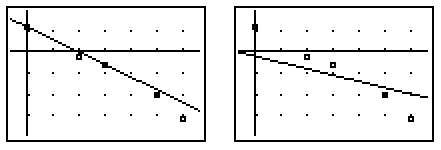
\includegraphics[width=0.7\linewidth]{least_squares}
\end{figure}

Hierdoor kan dus gesteld worden dat door $\beta$\textsubscript{0} en $\beta$\textsubscript{1} te vari\"{e}ren en te kijken welke parametercombinatie voor de curve zal zorgen waarvan de afstand van de datapunten en die curve het laagst is, bepaald kan worden welke waarden voor  $\beta$\textsubscript{0} en $\beta$\textsubscript{1} optimaal zijn.

De accuraatheid van een curve kan dus weergegeven aan de hand van formule 2.2.

\begin{equation}
Error = \sum(actual\;output - predicted\;output)^2
\end{equation}

Nu rijst de vraag hoe de parameters zodanig kunnen evolueren zodat ze de kleinst mogelijke foutmarge benaderen. Dit wordt gerealiseerd aan de hand van gradient descent een uitgebreide uitleg van gradient descent komt aan bod bij het bespreken van de LSTM techniek maar het komt er op neer dat gradient descent er zal voor zorgen dat de optimale parameters zo nauwkeurig mogelijk bepaald zullen kunnen met een zo laag gebruik van middelen.

%, dit wordt grafisch weergegeven op figuur 2.2 waarbij J($\theta_0\theta_1$) de foutmarge weergeeft en $\theta_0$ en $\theta_1$ de variabelen weergeven. Gradient descent zal er dan voor zorgen dat men in een dal zal terechtkomen en dus de parameters voor de laagste foutmarge bepaald kunnen worden. De stapgrootte waarmee afgedaald wordt is bij het minimaliseren van de foutmarge zeer belangrijk. Een grotere stapgrootte zullen de optimale parameters snel bepaald kunnen worden maar zullen ze niet nauwkeurig zijn. Terwijl een kleinere stapgrootte voor een heel hoge uitvoeringstijd zal kunnen zorgen maar wel zeer nauwkeurig zal zijn en je effectief in het laagste punt van het grafische dal zal terechtkomen. Gradient descent zal de stapgrootte verkleinen naargelang de foutmarge kleiner wordt en de optimale foutmarge dus op een nauwkeurige manier bepaald zal kunnen worden zonder relatief veel middelen te benutten.



\begin{table}[ht]
    \caption{Voorbeelddata voor lineaire regressie~\autocite{Pant2019}}
    \centering
    \begin{tabular}{|c|c|} 
        \hline     
        Living area (feet\textsuperscript{2}) & Price (1000\$) \\ [0.5ex] 
        \hline\hline
        2104 & 400 \\  [0.3ex]
        \hline
        1600 & 330 \\ [0.3ex]
        \hline
        2400 & 369 \\ [0.3ex]
        \hline
        1416 & 232 \\ [0.3ex]
        \hline
        3000 & 540 \\ [0.3ex]
        \hline
    \end{tabular}
    \label{Tab:Tcr}
\end{table}

\begin{figure}[!h]
    \centering
    \caption{Grafische weergaven voorbeelddata voor lineaire regressie~\autocite{Pant2019}}
    \label{fig:ExampleDataLinearRegressionGraph}
    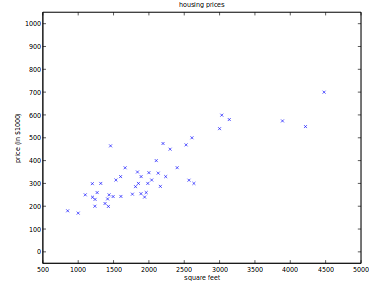
\includegraphics[width=0.7\linewidth]{ExampleDataLinearRegressionGraph}
\end{figure}

%\begin{figure}[!h]
%    \centering
%    \caption{Grafische weergave van gradient descent}
%    \label{fig:GradientDescend3D}
%    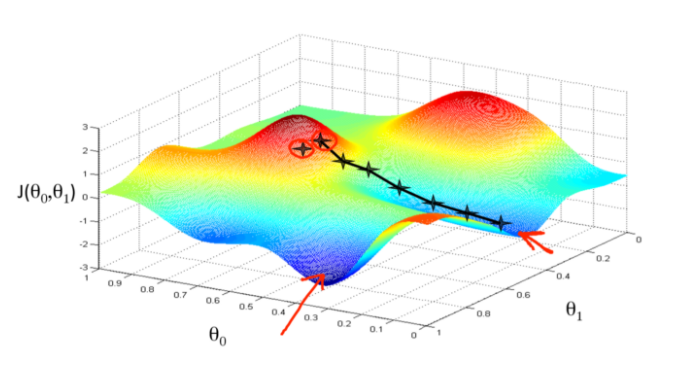
\includegraphics[width=0.7\linewidth]{GradientDescend3D}
%\end{figure}

\subsection{\IfLanguageName{dutch}{Polynomiale Regressie}{Polynomial Regression}}

Soms zal de foutmarge bij data hoog blijven bij lineaire regressie ook al is er een verband zichtbaar, dit verband zal dan waarschijnlijk niet te vatten vallen onder een gewone rechte. In zo'n geval kan polynomiale regressie hulp bieden, dit zal een complexere functie aan de data proberen fitten. Formule 2.3 is dan formule van een $2^{de}$ graadsfunctie 

\begin{equation}
y = \beta_0 + \beta_1 x_1  + \beta_2 x_2^2 
\end{equation}

Dit zorgt ervoor dat de algemene formule herleid wordt naar de formule 2.4 indien we een polynomiale vergelijken wensen toe te passen bij de regressieanalyse.

\begin{equation}
y = \beta_0 + \beta_1 x  + \beta_2 x^2 + ... + \beta_m x^m + residual\;error
\end{equation}

Ook bij polynomiale regressie wordt gebruik gemaakt van gradient descent om de minimale kost te berekenen aangezien dit in principe een uitbreiding is op lineaire regressie. 

Dus polynomiale regressie zal de beste gemiddelde inschatting kunnen maken van de relatie tussen de afhankelijke en onafhankelijke variabelen. De curve die gefit moet worden zal zeer complexere vormen dan een simpele rechte kunnen aannemen en meer dan enkel lineaire verbanden kunnen deduceren uit de data. Het grootste nadeel van polynomiale regressie is dat enkele uitschieters de resultaten sterk kunnen be\"{i}nvloeden terwijl er bij lineaire regressie meer validatietechnieken beschikbaar zijn voor het achterhalen van uitschieters \autocite{Pant2019}. 



\subsection{\IfLanguageName{dutch}{Logistische Regressie}{Logistic Regression}}

Logistische regressie is gelijkaardig aan lineaire regressie maar in tegenstelling tot lineaire regressie zal dit voornamelijk gebruikt worden voor classificatieproblemen, waarbij dus geen continue waarden dienen voorspeld te worden maar nominale waarden. Onder zijn meest simpele vorm zal dit type algoritme nuttig zijn bij het voorspellen van binaire waarden bijvoorbeeld indien men al dan niet aan een aandoening zal lijden. Dit wordt benoemd als binaire logistische regressie. Wanneer er 3 of meer categori\"{e}n die dienen voorspeld te worden waarvan de ene niet duidelijk hoger of lager is dan de andere zoals bijvoorbeeld type huisdier wordt dit benoemd als multinomial logistic regression. Indien er wel een logische ordening in zit zoals een aantal sterren op een filmbeoordeling wordt dit benoemd als ordinale logistische regressie.
Aangezien in deze paper enkel continue waarden voorspeld zullen worden, zal hier niet dieper op in gegaan worden~\autocite{Swaminathan2018}.

\subsection{\IfLanguageName{dutch}{Meervoudige lineaire regressie}{Multiple Linear Regression}}

Indien er meerdere onafhankelijke variabelen beschikbaar zijn die een lineaire invloed zouden hebben op de afhankelijke variabele kunnen deze ook in rekening gebracht worden. Dit model zal dan opgesteld worden aan de hand van meervoudige lineaire regressie ofwel multiple linear regression. Formule 2.5 geeft weer hoe de onafhankelijke waarden bij meervoudige lineaire regressie berekend zullen worden.

\begin{equation}
y_i = \beta_0 + \beta_1 {x_i}_1 + \beta_2 {x_i}_2 + ... + \beta_n {x_i}_n + \epsilon_i
\end{equation}

Net zoals bij enkelvoudige lineaire regressie zal $y\textsubscript{i}$ de afhankelijke variabele weergeven en $\beta$\textsubscript{0} het intercept. Het verschil zit hem in de termen die volgen want aangezien er rekening gehouden wordt met meerdere onafhankelijke variabelen, zullen ook deze verwerkt worden in de formule door middel van een waarde te voorzien voor elke onafhankelijke variabele weergegeven door $X\textsubscript{i}$ met bijhorend intercept weergegeven door $\beta$. De $n$ in de formule geeft dan het aantal onafhankelijke variabelen weer. De $\epsilon$\textsubscript{i} zal ook in dit geval een factor zijn die rekening zal houden met de meetfouten~\autocite{Kenton2020}.

\subsection{\IfLanguageName{dutch}{Toepassing}{}}

Deze regressietechnieken zullen dienen als basis voor andere meer uitgebreide technieken zoals ARIMA maar de verbanden die ze weergeven zijn te eenvoudig om effectief te gebruiken voor het opbouwen van modellen om aan extrapolatie te doen.~\autocite{Sinha2019} Daarom zullen de klassieke regressiemethodes niet toegepast worden bij deze bachelorproef. 

%\subsection{\IfLanguageName{dutch}{Meervoudige polynomiale regressie}{Multiple Polynomial Regression}}

\section{\IfLanguageName{dutch}{ARIMA}{Prediction Techniques}}
\label{sec: Theoretische toelichting over ARIMA}

ARIMA is een modeleringstechniek die voorspellingen maakt op basis va, stationaire en gedifferenti\"{e}erde data. Daarom worden deze begrippen eerst toegelicht alvorens de techniek zelf te bespreken. 

\subsection{\IfLanguageName{dutch}{Stationariteit}{Stationarity}}

Een stationaire tijdreeks is een tijdreeks waarvan de eigenschappen niet afhankelijk zijn van het tijdstip waarop de reeks wordt geobserveerd~\autocite{Hyndman2018}. Indien er een duidelijke trend dus een algemene stijging of daling aanwezig is zal de tijdreeks niet stationair zijn. Ook wanneer er een seizoensverband aanwezig is die lijkt op een sinus of cosinusfunctie wordt de data als niet stationair beschouwd. Wanneer er echter een cyclisch verband aanwezig is kan er een speciaal type ARIMA model gebruikt worden dat rekening zal houden met deze seizoenscomponent genaamd SARIMA deze zal zodadelijk toegelicht worden.
In figuur \ref{fig:stationarity} zijn enkele voorbeeldtijdreeksen zichtbaar dit toont aan dat het niet zo evident is om te bepalen welke tijdreeks stationair is.

\begin{figure}[!h]
    \centering
    \caption{Voorbeeldtijdreeksen~\autocite{Hyndman2018}}
    \label{fig:stationarity}
    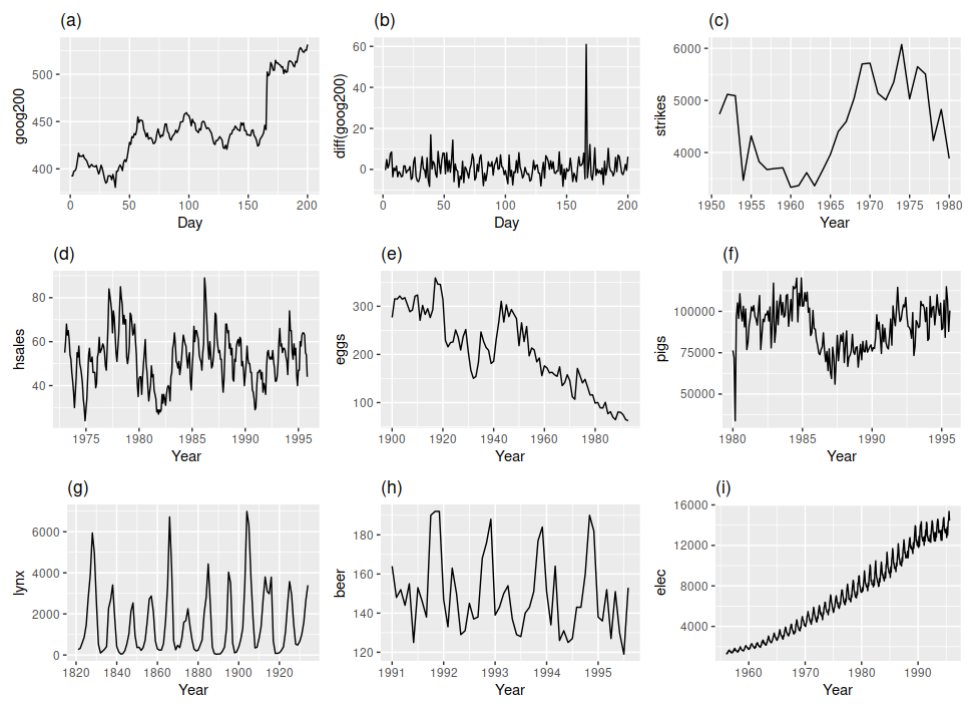
\includegraphics[width=0.7\linewidth]{stationarity}
\end{figure}

De cijfers in de figuur omschrijven de volgende data:

\begin{enumerate}[label=(\,\alph*)\,]
    \item De aandeelkoersen van Google voor 200 opeenvolgende dagen
    \item De dagelijkse veranderingen in de aandeelkoersen van Google voor 200 opeenvolgende dagen
    \item Het jaarlijkse aantal stakingen in de Verenigde Staten
    \item Maandelijkse verkoop van nieuwe gezinswoningen in de Verenigde Staten
    \item Jaarlijkse prijs van een dozijn eieren in de Verenigde Staten (rekening houdend met inflatie)
    \item Maandelijks aantal varkens die geslacht worden in Victoria, Australi\"{e}
    \item Jaarlijks aantal lynxen die opgesloten worden in het McKenzie River district van noordwest Canada
    \item Maandelijkse Australische bierproductie
    \item Maandelijkse Australische elektriciteitsproductie
\end{enumerate}

\subsection{\IfLanguageName{dutch}{Seizoenseffect}{Seasonality}}

Bij de figuren (d), (h) en (i) is er een duidelijk seizoenseffect zichtbaar. Er vallen duidelijke trends waar te nemen op figuren (a), (c), (e), (f) en (i). Ook in figuur (g) lijkt er een duidelijk seizoenseffect te zijn, maar deze veranderingen zijn aperiodisch dus op lange termijn valt dit niet te voorspellen aldus is deze tijdreeks stationair.


\subsection{\IfLanguageName{dutch}{Differentiatie}{Differencing}}

Aan de hand van deze grafieken kan ook een ander begrip toegelicht worden dat een belangrijk gegeven is bij het opstellen van een ARIMA model namelijk differentiatie. Zo wordt op figuur (a) de aandeelkoers van google weergegeven voor 200 opeenvolgende dagen, maar hier is een duidelijk stijgende trend zichtbaar. Hierdoor kan de data niet op deze manier ge\"{i}nterpreteerd worden door een ARIMA model. Maar we kunnen de data op een andere manier voorstellen namelijk door de koerswissellingen zoals weergegeven wordt op figuur (b) waardoor er geen trend meer aanwezig zal zijn en nog steeds geen zichtbare seizoensgebondenheid aanwezig is. 

\subsubsection{\IfLanguageName{dutch}{Random walk differentiatie}{Random walk model}}
Bij random walk differencing wordt de data gediffernti\"{e}erd door het verschil te nemen tussen een tijdstap en de tijdstap die ervoor komt. Dit zal de evolutie van de tijdreeks weergeven en aangeven hoeveel een waarde precies verschilt van de tijdstap ervoor. Deze differentiatie kan uitgedrukt worden als

\begin{equation}
y_t^\prime = y_t - y_{t-1}.
\end{equation}

De gedifferenti\"{e}erde reeks zal 1 waarde minder hebben dan de originele serie omdat er geen waarde voor de eerste $y_1^\prime$ komt om deze te differenti\"{e}ren.
 
Wanneer de gedifferentiëerde reeks ruis is kan het model uitgedrukt worden als 
 
\begin{equation}
y_t - y_{t-1} = \epsilon_t,
\end{equation}

Hierbij zal $epsilon_t$ de ruis weergeven. Door deze formule te hervormen bekomen we het ''random walk model".

Deze modellen worden vaak gebruikt voor niet-stationaire data, voornamelijk bij financi\"{e}le en economische toepassingen.

De voorspellingen van dit model zijn gelijk aan dit de laatste observatie.

\subsubsection{\IfLanguageName{dutch}{Tweedegraadsdifferentiatie}{Second order differencing}}

In sommige gevallen zal gedifferencieerde data nog steeds niet stationair zijn dan is het eventueel mogelijk om de gedifferenti\"{e}erde nogmaals te differenti\"{e}ren. Dit kan als volgt geformuleerd worden.

\begin{equation}
\begin{aligned}
y_t^n {} & = y^\prime_t - y^\prime_{t-1}  \\
& = (y_t - y_{t-1}) - (y_{t-1} - y_{t-2})\\
& = y_t - 2y_{t-1} - y_{t-1}
\end{aligned}
\end{equation}

Op deze manier kan een verandering in de veranderingen gedetecteerd worden. Uiteraard zou men nog een stap verder kunnen gaan maar dit blijkt in praktijk zo goed als nooit nodig te zijn.

\subsubsection{\IfLanguageName{dutch}{Seizoensdifferentiatie}{Seasonal differencing}}
Een laatste manier om data te differenti\"{e}ren is seizoensdifferentiatie. Hierbij zal telkens het verschil genomen worden van een tijdstap en diezelfde tijdstap van de vorige seizoenscyclus. Dit kan als volgt weergegeven worden,

\begin{equation}
y_t^\prime = y_t - y_{t-m}.
\end{equation}

Hier zal $m$ slaan op het aantal observaties in een seizoen. Indien deze data, die seizoensgedifferenci\"{e}erd is, ruis blijkt te zijn dan zou een geschat model voor de originele data kunnen geformuleerd worden als

 \begin{equation}
y_t - y_{t-m} = \epsilon_t,
 \end{equation}

Om seizoensdifferentiaties en gewone differentiaties uit elkaar te houden worden gewone differentiaties ook benoemd als eerste differentiaties. 

Het is mogelijk dat deze verschillende soorten differentiaties gecombineerd moeten worden om tot een stationaire dataset te komen. Een dataset waarbij het waarschijnlijk nodig zal zijn om eerste differentiaties en seizoensdifferentiaties gecombineerd moeten worden is die van de maandelijkse Australische elektriciteitsproductie zichtbaar op figuur \ref{fig:stationarity} (i). Aangezien er een seizoenscyclus en een stijgende trend aanwezig is.

\subsection{\IfLanguageName{dutch}{Toeliching ARIMA}{}}

ARIMA is een acroniem gevormd door AutoRegressive Integrated Moving Average wat vrij vertaald kan worden als het autoregressie ge\"{i}ntegreerde voortschrijdend gemiddelde. Deze benaming geeft ook onmiddellijk de sleutelaspecten van dit model weer. 

Zo staat autoregressief voor het modelleren van een volgende stap in een sequentie als een lineaire functie op basis van de voorgaande waarden in deze sequentie.
\\Daarnaast is ARIMA ook een ge\"{i}ntegreerd model wat inhoudt dat niet de cumulatieve waarden gebruikt worden om voorspellingen te maken maar er gekeken wordt naar het verschil tussen die cumulatieve waarden.
\\Ten slotte wordt ook gekeken naar het voortschrijdend gemiddelde in plaats van naar de ruwe data zelf dit zal ervoor zorgen dat extreme waarden veroorzaakt door anomaliteiten geneutraliseerd worden. Hierdoor zal de globale trend beter waarneembaar zijn.

ARIMA modellen zijn theoretisch gezien, de meest algemene klasse van modellen om een tijdreeks te voorspellen die stationair/stationary gemaakt kan worden. 

Elk van deze componenten is geparameteriseerd en kan dus aangepast worden deze parameters worden benoemd als ($p$, $d$ \& $q$)

$p$: Het aantal verlate observaties die worden opgenomen in het model. Deze worden in het Engels benoemd als lag observations of lag order.
\\$d$: Zal bepalen hoeveel keer ruwe observaties van elkaar afgetrokken worden dit kan ook benoemd worden als de mate van differentiatie of the degree of differencing in het Engels.
\\$q$: Deze parameter zal het aantal tijdstappen waarvan het voortschrijdend gemiddelde genomen wordt aangeven. Deze wordt in het Engels benoemd als the order of moving average. 

Een lineair regressiemodel wordt geconstrueerd met data waarbij er een graad van differentiatie is zodat deze stationair is. Dit houdt in dat trend en seizoensstructuren die het regressiemodel op een negatieve manier be\"{i}nvloeden verwijderd worden.

Bij elke parameter kan ook de waarde 0 opgegeven worden zodat dit aspect horende bij die parameter buiten beschouwing gelaten wordt en dit model effectief gebruikt kan worden als gelijk welke combinatie zoals bijvoorbeeld een autoregressief en een ge\"{i}ntegreerd model al dan niet gebruikmakend van het voortschrijdend gemiddelde~\autocite{Brownlee2018}.

$d$ zal dus de differentiatiegraad weergeven wanneer we hier rekening mee houden kunnen we stellen dat de formule voor ARIMA er als volgt uit zal zien~\autocite{Nau2020}:

\begin{equation}
\hat{y_t} = \mu + \phi_1 y_{t-1} + ... + \phi_p y_{t-p} + \theta_1 \epsilon_{t-1} - ... - \theta_q \epsilon_{t-q}
\end{equation}

Om de werking van ARIMA te schetsen zullen kort enkele basisparametercombinaties toegelicht worden.

\subsubsection{ARIMA(1,0,0)}

Dit zal een autoregressief model van de eerste orde zijn ofwel een first-order autoregressive model. Deze parametercombinatie zal gebruikt worden als de reeks stationair en autogecorreleerd is. Dit zou dus voorspeld kunnen worden door de eigen waarde te nemen en deze op te tellen met een constante. De voorspellingsvergelijking zal er als volgt uit zien:

\begin{equation}
\hat{y_t} = \mu + \phi_1 y_{t-1}
\end{equation}

Dit stelt voor dat er regressie uitgevoerd en kan benoemd worden als een ARIMA(1,0,0) model. Wanneer het gemiddelde van $y$ gelijk is aan nul, zal de constante term achterwege gelaten worden. Indien de hellingsco\"{e}fficient $\phi_1$ positief maar minder dan \'{e}\'{e}n is zal het model de waarde van de volgende periode voorspellen als $\phi_1$ keer zo ver van het gemiddelde dan de waarde van deze periode. 

Indien men een autoregressief model van de 2\textsuperscript{de} orde wil voorstellen zal er bij formule (2.12) rechts een $y_{t-2}$ term toegevoegd worden. Wanneer men een model van nog hogere orde wenst voor te stellen dient men analoog termen toe te voegen. Afhankelijk van de tekens en de grootte van de co\"{e}fficienten zal een ARIMA(2,0,0) model een systeem onderschrijven waarvan de gemiddelde omkering sinuso\"{i}daal oscillerend zal zijn, wat te vergelijken valt met de beweging van massa aan een veer die onderhevig is aan willekeurige uitwijkingen.


\subsubsection{ARIMA(0,1,0)}

Deze vorm van ARIMA past de meest simpele vorm van differentiatie toe namelijk ``random walk'', hierbij zal de eerste differentiatie die zonet besproken is in de sectie differentiatie toegepast worden op de data. Door middel van deze differentiatie kan niet-stationaire data omgevormd kunnen worden naar stationaire data indien dit nog steeds niet het geval is kan deze data in een hogere graad gedifferenci\"{e}erd worden. Dit kan weergegeven onder de vorm van deze formule:

\begin{equation}
\hat{y_t} = \mu + y_{t-1}
\end{equation}

Hier zal de constante term $\mu$ de gemiddelde verandering van periode tot periode weergeven dit kan ook benoemd worden als de ``long term drift'' in $y$. Aangezien het enkel een niet-seizoensgebonden verschil en en een constante term omvat wordt het geclassificeerd als een ``ARIMA(0,1,0) model met constante''. Een random walk zonder drift model zou een ARIMA(0,1,0) model zonder constante zijn.


\subsubsection{ARIMA(1,1,0)}

Deze ARIMA configuratie staat voor een gedifferenci\"{e}erd autoregressief model van de eerste graad. Indien de fouten van een random walk model autogecorreleerd zijn is het mogelijk dat dit verholpen kan worden door een vertraging ofwel lag toe te voegen aan de afhankelijke variabele van de voorspellingsvergelijking. Zo zou dus regressie uitgevoerd worden op het eerste verschil van $y$ en zichzelf, vertraagd met 1 tijdstap. Hierbij zal de vergelijking er als volgt uitzien:

\begin{equation}
\hat{y_t} = \mu + y_{t-1} + \phi_1 (y_{t-1} - y_{t-2})
\end{equation}

\subsubsection{ARIMA(0,1,1)}

Hier wordt de laatste parameter van ARIMA voor het eerst aangesproken de $q$. Hierdoor zal er nu gewerkt worden met een voortschrijdend gemiddelde van de data. Dit zal er voor zorgen dat ruis iets meer geneutraliseerd wordt.

\begin{equation}
\hat{y_t} = \mu + y_{t-1} - \theta_1 e_{t-1}
\end{equation}

De constante $\mu$ kan eventueel achterwege gelaten worden, deze zal er voor zorgen dat de voorspelling op lange termijn eerder hellend zal zijn hierbij zal het ook mogelijk zijn om een negatieve co\"{e}fficient toe te laten. Deze constante zorgt er ook voor dat het ARIMA model een SES model wordt. Indien hier niet voor gekozen wordt zal de voorspelling op lange termijn vlak zijn. Zonder constante wordt dit type model benoemd als simple exponential smoothening indien er een constante gebruikt wordt hier growth aan toegevoegd, wat wijst op de stijgende trend op lange termijn waarvan de helling gelijk is aan $\mu$.

\subsubsection{ARIMA(0,2,1) of ARIMA(0,2,2)}

Deze configuraties zonder constante worden ook benoemd als lineaire exponenti\"{e}le afvlakking. Hier zal de 2\textsuperscript{de} afgeleide genomen worden omwille van de waarde voor $d$. 

\begin{equation}
\hat{y_t} = 2y_{t-1} - y_{t-2} - \theta_1 e_{t-1} - \theta_2 e_{t-2}
\end{equation}

De $\theta_1$ en $\theta_2$ zullen staan voor de MA(1) en MA(2) co\"{e}fficienten. Dit zal overeenkomen met Holt's model en in speciale gevallen met Brown's model. het zal gebruik maken van exponenti\"{e}le gewogen voortschrijdende gemiddeldes om het lokale niveau en lokale trend (local level and local trend) te schatten. Voorspellingen op lange termijn zullen naar een rechte lijn toe convergeren wiens helling zal afhangen van de gemiddelde trend naar het einde van de reeks toe. 

\subsubsection{ARIMA(1,1,2)}

Dit wordt benoemd als damped-trend linear exponential smoothing en wordt weergegeven door de formule:

\begin{equation}
\hat{y_t} = y_{t-1} + \phi_1 (y_{t-1} - y_{t-2}) - \theta_1 e_{t-1} - \theta_2 e_{t-2}
\end{equation}

Dit model zal de lokale trend aan het einde van de reeks extrapoleren maar zal afvlakken naar het einde toe. 

Bij het opstellen van een ARIMA mode wordt aangeraden om een van de parameters $p$ of $q$ niet groter te laten worden dan 1 aangezien er een hoge waarschijnlijkheid is dat dit zal leiden tot overfitting of andere fouten.

Een manier om de corelaties en een eventueel vertraagd effect te identificeren tussen de waarden rekening houdend met trend, seasonality en het residu is een ACF ofwel een auto-corelation function~\autocite{Salvi2020}.

Een aanvulling daarop is een PACF ofwel een partial auto-correlation function deze zal eventuele correlaties wanneer de effecten na eerdere vertragingen verwijderd worden (door middel van ACF) weergeven. 

Een goede vuistregel bij het opstellen van een ARIMA model is het verhogen van de $p$ indien er een positieve correlatie is dit houdt in dat de afhankelijke variabele zal stijgen als de onafhankelijke variabele stijgt. Wanneer er een negatieve corelatie is en de onafhankelijke variabele stijgt zal de afhankelijke variabele dalen en in dit geval is het beter om de $q$ te verhogen.

Een stappenplan om ARIMA toe te passen op een dataset zal er als volgt uit zien:

\begin{enumerate}
    \item Plot de data en identificeer ongewone waarden
    \item Transformeer de data om de variantie te stabiliseren indien nodig
    \item Als de data niet stationair is neem eerste differentiaties van de data totdat deze stationair is.
    \item Onderzoek de ACF/PACF en kijk of een ARIMA(p,d,0) of ARIMA(0,d,q) model gebruikt moet worden
    \item Test de modellen uit en gebruik AICc (een scoringstechniek) om het model te verbeteren.
    \item Bekijk de residuen van het gekozen model door ze te plotten samen met de ACF en een portmanteau test van de residuen te doen. Indien deze er niet uitzien als ruis is het aangeraden een nieuw model te proberen
    \item Wanneer de residuen er uitzien als ruis kunnen voorspellingen gemaakt worden   
\end{enumerate}


\subsection{\IfLanguageName{dutch}{Varianten op ARIMA}{Variants of ARIMA}}

\subsubsection{\IfLanguageName{dutch}{SARIMA}{SARIMA}}

In sommige gevallen blijkt er een seizoensgebondenheid aanwezig te zijn in de data. Deze seizoensgebondenheid zal zorgen voor constante fluctuaties.
Deze manier van be\"{i}nvloeden is iets waar bij een gewoon ARIMA model geen rekening mee wordt gehouden. Daarom is er een variant op het ARIMA model genaamd SARIMA waarbij de toegevoegde S zal staan voor de seizoensgebondenheid. Dit zal in rekening gebracht worden door extra parameters toe te voegen. Zo zullen de parameters bij ARIMA $(p,d,q)$ zijn, terwijl de parameters bij SARIMA $(p, d, q)(P, D, Q)m$ zijn, waarbij $m$ zal staan voor het aantal tijdsstappen binnen een seizoenscyclus. Zo zal bij een jaarlijkse cyclus $m$ gelijk zijn aan 12 als de tijdspanne tussen de observaties 1 maand bedraagt. Daarnaast zal de $p$ staan voor autoregressieve seizoensorde ofwel de seasonal autoregressive order, $d$ voor de gedifferenc\"{i}eerde seizoensorde ofwel de seasonal difference order en $q$ voor de seizoensorde van het voortschrijdend gemiddelde ofwel de seasonal moving average order ~\autocite{Brownlee2018a}.

\subsubsection{\IfLanguageName{dutch}{VARMAX}{VARMAX}}
Wanneer er meerdere tijdsreeksen voorspeld moeten worden waarbij er een verband mogelijk zou kunnen zijn tussen de verschillende tijdsreeksen kan de VARMAX techniek gebruikt worden. Hierbij zal de V staan voor vector wat duidt op het interpreteren en voorspellen van vectoren. Dit type model zal dan ook gebruikt worden bij het voorspellen van multivariate of meervoudige tijdreeksen AR wijst andermaal op autoregressief. MA slaat ook weer op het voortschrijdend gemiddelde. De X in VARMAX staat voor de invloed van exogene factoren op de factoren die voorspeld moeten worden. 

\section{\IfLanguageName{dutch}{Long Short Term Memory}{Prediction Techniques}}
\label{subsubsec: Theoretische toelichting van long short term memory netwerken (LSTM)}

Als tweede methode die gebruikt zal worden om tijdreeksen te voorspellen wordt gekozen voor een recurrent neuraal netwerk met gebruik van Long Short Term Memory modellen wat afgekort wordt als LSTM.

Een recurrent neuraal netwerk zal uitgebreid toegelicht worden in de volgende secties maar dit kan kort omschreven worden als een structuur die gebruik maakt van trainingsdata om te ``leren'' en op basis van dit leerproces voorspellingen kunnen maken van nieuwe data. Om dit met een simpel voorbeeld te schetsen zou een neuraal netwerk net zoals wij als mens leren dat er bij veel bewolking kans zal zijn op regen. Om dit te realiseren zullen alle parameters echter numeriek doorgegeven moeten worden aan het neuraal netwerk in dit geval zou een soort van bewolkingsgraad aangewezen zijn. Op basis daarvan zal het neuraal netwerk dan een kans op regen kunnen aangeven. 

Een LSTM is een type recurrent neuraal netwerk dat gebruikt wordt bij sequenti\''{e}le voorspellingsproblemen. Dit betekent dat de volgorde van de data een rol zal spelen en dat bij het voorspellen van een waarde in een reeks rekening zal gehouden worden met een aantal waarden die vlak voor de te voorspellen waarde komen. 


\subsection{\IfLanguageName{dutch}{Theoretische toelichting}{}}
\label{subsec: Theretische toelichting van long short term memory netwerken (LSTM)}

Een neuraal netwerk valt makkelijkst te vergelijken met een menselijk brein. Zo zullen wij bijvoorbeeld het cijfer 1 herkennen aan zijn vormen. Door de verschillende pixels, gebruikt voor het weergeven van ons cijfer 1 als inputwaarden voor een neuraal netwerk te gebruiken en de outputwaarden gelijk te stellen met cijfers 0 tot en met 9 kan het netwerk aangeleerd worden deze cijfers te herkennen. 

Dit gebeurt niet vanzelf maar door een combinatie van eenvoudige rekeneenheden die verbonden zijn en waartussen er verbindingen zijn die beschreven worden met een re\"{e}el getal dat de sterkte van een verbinding aangeeft~\autocite{Lievens2018a}. Zo'n combinatie van eenvoudige rekeneenheden die ook benoemd worden als neuronen wordt net zoals bij het menselijk brein een neuraal netwerk genoemd dit wordt weergegeven op figuur \ref{fig:neuron}. 

\begin{figure}
    \centering
    \caption{Voorstelling van een neuron die invoer ontvangt van 3 andere neuronen ~\autocite{Lievens2018a}}
    \label{fig:neuron}
    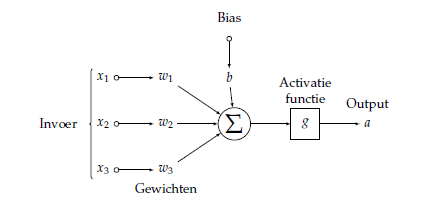
\includegraphics[width=0.7\linewidth]{neuron}
\end{figure}

Zo bevinden zich tussen de input en de outputlaag verschillende lagen die benoemd worden als verborgen lagen. In deze lagen bevinden zich knooppunten (neuronen) waarin waarden worden berekend die een interpretatie geven van de inputwaarden waarmee ze verbonden zijn. Wanneer we dit toepassen op ons voorbeeld zou in een knooppunt bijvoorbeeld kunnen bekeken worden of er in het midden van de te interpreteren pixels een lijn staat. Wanneer dit het geval zou zijn zou er in dit neuron een grote waarde weergegeven worden en zal deze een sterk signaal sturen. Wanneer we voor dit voorbeeld met 1 verborgen laag zouden werken zou het neuron dat een sterk signaal zendt bij het herkennen van een centrale verticale lijn een belangrijke waarde zijn voor het herkennen van een 1 en een 4. De sterke van dit signaal zal dus een grote invloed hebben op de kans dat het resultaat een 1 of een 4 is.
Wanneer we hier dieper op ingaan kunnen we aan elk neuron een formule toewijzen die er zo uitziet:

\begin{equation}
n=w_1 i_1+w_2 i_2
\end{equation}

W staat voor de gewichten, $i$ staat voor de inputwaarde. Stel dat bij dit neuron de bovenste 3 pixels genomen worden en we voor de eenvoud werken met een 3x3 afbeelding, dan zal de formule er als volgt uitzien:

\begin{equation}
n=w_1 i_1+w_2 i_2+ w_3 i_3
\end{equation}

$n$ zal dan staan voor gewogen gemiddelde, door hier een bias aan toe te voegen $b$ net zoals bij lineaire regressie en dit als invoer te gebruiken voor een activatiefunctie $g$ zal de sterkte van het uitvoersignaal bekomen worden. 


Indien een neuron effectief geactiveerd wordt zal bepaald worden door de volgende formule.

\begin{equation}
a = g(n + b)
\end{equation}

Een bias $b$ zal bij een neuraal netwerk zorgt voor een correcte neutrale toestand binnen een neuraal netwerk wanneer alle features nul zijn net zoals bij lineaire regressie.  

Door het gebruik van een activatiefunctie $g$ zal dit netwerk ook meer beginnen lijken op de werking van neuronen zoals ze voorkomen in de natuur. 

Een activatiefunctie zal gebruikt worden om voor non-lineariteit te zorgen binnen het model. Wanneer we de activatiefunctie zouden laten wegvallen zou het volledige neurale netwerk kunnen herleid worden tot \'{e}\'{e}n lineaire functie waardoor er enkel weer lineaire verbanden gelegd kunnen worden. Het toevoegen van een activatiefunctie zal er voor zorgen dat de lineariteit gebroken wordt en er binnenin het netwerk nieuwe, abstracte features gegenereerd kunnen worden die kunnen resulteren in een betere interpretatie van de invoerdata.



\paragraph{Toepassing}
Bij dit voorbeeld zijn we nog steeds op zoek naar een 1 en kennen een hoge waarde toe aan donkere kleuren opdat het model de afbeelding zou kunnen interpreteren. Dit zou betekenen dat $i_1$ en $i_3$ een lage waarde moeten hebben en $i_2$ een hoge waarde. In dit geval zullen de gewichten voor $w_1$ en $w_3$ gelijkgesteld worden aan -1 en het gewicht voor $w_2$ aan 1. Daardoor zal n een hoge waarde krijgen als de centrale pixel zwart is en de buitenste pixels wit. Dit wordt de propagation function genoemd. Om deze waarden om te zetten naar een waarde die interpretabel is doorheen het volledige model wordt het resultaat van de propagation function nog eens gebruikt als invoerwaarde voor een activatiefunctie. In dit geval zou de hyperbolic tangent (tanh) een goede keuze zijn, maar dit hangt af van de toepassing.
Bij dit voorbeeld zou dat signaal dan naar de outputlaag gestuurd worden die op zijn beurt ook weer diezelfde formule toepast maar dan niet met de invoerwaarden maar met de resultaten uit de verborgen laag. Hieruit zal dan een score zou komen die aangeeft hoe waarschijnlijk het is dat de waarden die de pixels weergeven uit de invoerlaag het cijfer vormen dat toegekend is aan dit neuron in de uitvoerlaag. 

Deze toepassing waarbij een cijfer wordt herkend is een voorbeeld van een toepassing van voorwaards gerichte neurale netwerken omdat de data slechts in 1 richting verloopt, een resultaat wordt niet be\"{i}nvloed door voorgaande inputwaarden. Bij recurrente neurale netwerken is dit wel het geval. Hierbij wordt rekening gehouden met de beoordelingen van voorgaande inputwaarden een voorbeeld hiervan is het beoordelen van zinnen de volgorde van de ingevoerde woorden zal een rol spelen. Zo zal `eet ik` ge\"{i}nterpreteerd kunnen worden als een vraag aan de hand van de woordanalyse. Terwijl 'ik eet' zal beoordeeld worden als een statement. 

Dit zal louter gebeuren op basis van de woordvolgorde waarbij connecties tussen verschillende cellen teruglopend kunnen zijn onder elkaar en de vorige inputwaarden dus een invloed zullen hebben op de beoordeling van de volgende inputwaarden~\autocite{Lievens2018a}.

Dit is dus een gelijkaardige werking aan voorwaarts gerichte neurale netwerken maar de signalen verlopen niet allemaal in dezelfde richting binnen het netwerk. Zo kan er een signaal van de 2\textsuperscript{de} verborgen laag teruggestuurd worden naar de 1\textsuperscript{ste} verborgen laag. Op die manier hebben de waarden van vorige iteraties een impact op de volgende resultaten en dit is wat we willen bereiken. 

Een lus van eenzelfde stuk uit het neuraal netwerk die informatie van vorige iteraties doorgeeft aan zichzelf dit wordt weergegeven op Figuur \ref{fig:lstmfig1}.

\begin{figure}[!h]
    \centering
    \caption{Cel in een neuraal netwerk dat gegevens van een andere cel gebruikt om een nieuw signaal uit te sturen~\autocite{Olah2015}}
    \label{fig:lstmfig1}
    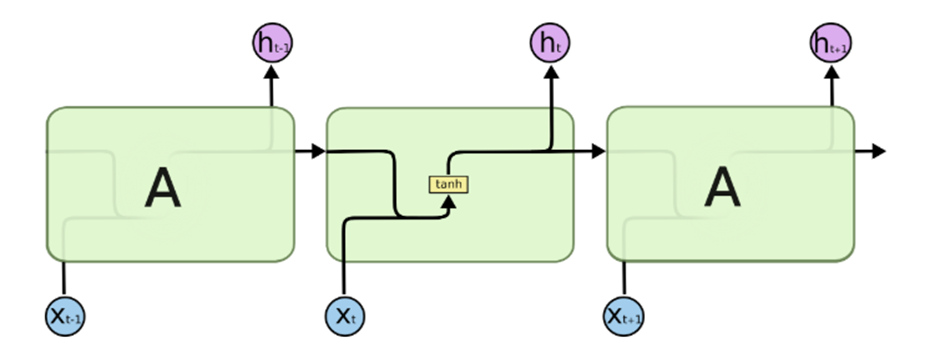
\includegraphics[width=0.7\linewidth]{lstmFig1}
\end{figure}

Om het verloop van een tijdreeks te voorspellen moet ook rekening gehouden worden met het tijdsverloop. Zo zal het verloop van de vorige dagen een invloed hebben op het verloop van de volgende dagen. Dus voor deze toepassing zullen recurrente neurale netwerken gebruikt worden aangezien voorwaarts gerichte neurale netwerken geen rekening houden met de voorgaande inputwaarden. 

Het probleem bij gewone recurrente neurale netwerken is dat deze moeilijk patronen herkennen op lange termijn. Hiervoor biedt de long short term memory variant van recurrente neurale netwerken een oplossing. Dit zorgt ervoor dat enkel de data die bijgehouden moet worden uit vorige iteraties een impact zal hebben op nieuwere resultaten. De werking van een LSTM wordt voorgesteld op figuur \ref{fig:lstmfig2}.

\begin{figure}[!h]
    \centering
    \caption{Gedetaileerdere figuur van een cel uit een neuraal netwerk dat informatie interpreteert uit een andere cel van het neurale netwerk~\autocite{Olah2015}}
    \label{fig:lstmfig2}
    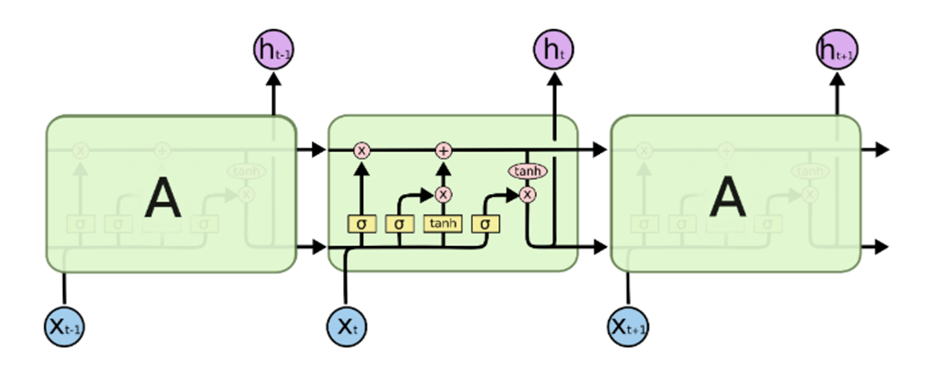
\includegraphics[width=0.7\linewidth]{lstmFig2}
\end{figure}


Dit aan de hand van 4 stappen:
\subparagraph{Stap 1}
Eerst wordt bepaald welke info weggegooid mag worden in de ``forget layer''.
Deze zal een waarde tussen 0 en 1 uitvoeren waarbij een 0 zal betekenen dat deze waarde volledig genegeerd mag worden voor elke component van de cell state en waarbij een 1 zal betekenen dat alles behouden zal moeten worden. 

\begin{figure}
    \centering
    \caption{Grafische weergave van de forget layer binnen het neuron~\autocite{Olah2015}}
    \label{fig:lstmfig3}
    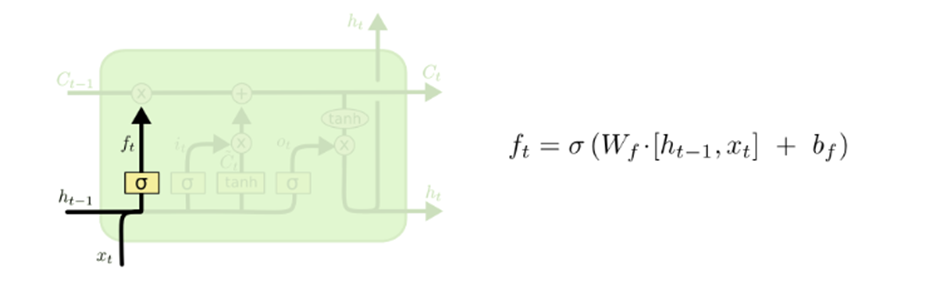
\includegraphics[width=0.7\linewidth]{lstmFig3}
\end{figure}


\subparagraph{Stap 2}
Voor de volgende stap zal in de ``input gate layer'' bepaald worden welke waarden ge\"{u}pdatet moeten worden aan de hand van een sigmo\"{i}de funtie die hier zal resulteren in $i_t$. Daarna zal de vector geconstrueerd worden met de potenti\"{e}le waarden $\tilde{C}_t$.

\begin{figure}
    \centering
    \caption{Grafische weergave van de input gate layer binnen het neuron~\autocite{Olah2015}}
    \label{fig:lstmfig4}
    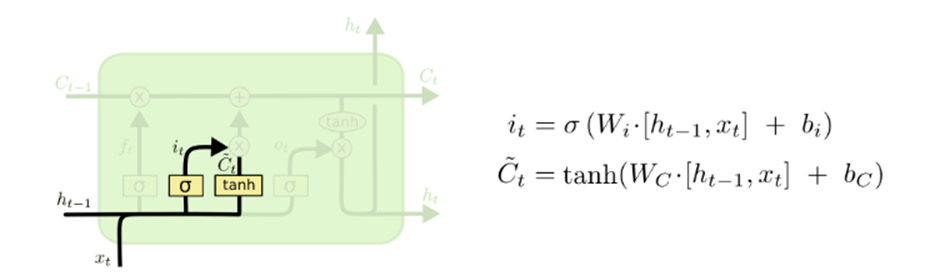
\includegraphics[width=0.7\linewidth]{lstmFig4}
\end{figure}

\subparagraph{Stap 3}
In deze stap zullen we de voorgaande celwaarde vernieuwen. Zo zullen door $C_{t-1}$ te vermenigvuldigen met $f_t$ de overbodige waarden vergeten worden. En door het product van $i_t$ en $C_t$ hierbij op te tellen zullen de achterhaalde waarden ge\"{u}pdatet worden. 

\begin{figure}
    \centering
    \caption{Grafische weergave van het $2^{de}$ deel van de input gateway~\autocite{Olah2015}}
    \label{fig:lstmfig5}
    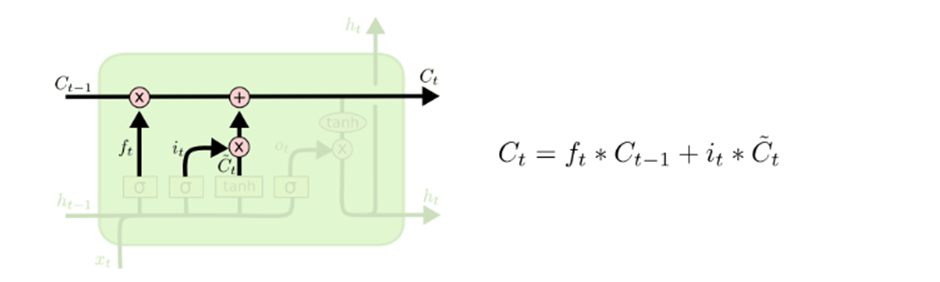
\includegraphics[width=0.7\linewidth]{lstmFig5}
\end{figure}

\subparagraph{Stap 4}
Als laatste zal de uitvoer bepaald worden. Dit is een gefilterde versie van de celtoestand. Die filtering gebeurt aan de hand van een sigmo\"{i}de functie. Het resultaat hiervan wordt dan vermenigvuldigd met de tanh van de celtoestand. Met deze formule verkrijgen we de uitvoerwaarde die de cyclus kan verderzetten.  

\begin{figure}
    \centering
    \caption{Grafische weergave van het onderdeel van de cel waarin de input vermenigvuldigd wordt met de tanh van de celtoestand om de outputwaarde te bekomen~\autocite{Olah2015}}
    \label{fig:lstmfig6}
    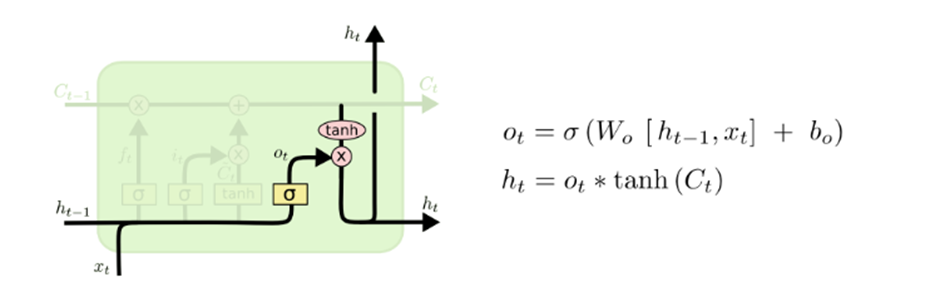
\includegraphics[width=0.7\linewidth]{lstmFig6}
\end{figure}

\subsection{\IfLanguageName{dutch}{Praktische toelichting}{Prediction Techniques}}
\label{subsec: Praktische toelichting van long short term memory netwerken (LSTM)}

Deze praktische toelichting is gebaseerd op het artikel van Jason Brownlee ~\autocite{Brownlee2018b} en zal dienen als basis voor het opstellen van een LSTM netwerk.

\subsubsection{\IfLanguageName{dutch}{Univariate LSTM modellen}{Univariate LSTM models}}

Univariate LSTM models maken voorspellingen voor data waarbij er slechts 1 afhankelijke variabele is.
Hierbij bestaan de problemen uit een reeks observaties. Op basis van vorige waarden in een reeks zal de volgende waarde in diezelfde reeks voorspeld worden. In deze subsectie zullen de voorgestelde modellen toegepast worden op eenstaps univariate tijdreeksen maar deze kunnen makkelijk aangepast worden om gebruikt te worden bij andere soorten tijdreeksen.

\subparagraph{\IfLanguageName{dutch}{Datavoorbereiding}{Data preparation}}
Een tijdreeks zelf bestaat uit een sequentie van waarden zoals hieronder bijvoorbeeld.
\lstset{caption={Originele datasequentie}}
\begin{lstlisting}[language=Python]
[10, 20, 30, 40, 50, 60, 70, 80, 90]
\end{lstlisting}

Om deze waarden te gebruiken voor het trainen van het neuraal netwerk zal deze tijdreeks omgevormd moeten worden naar samples. De dimensies van deze samples zullen bepalen hoeveel inputwaarden en outputwaarden zullen gebruikt worden bij het model. Aangezien we bij dit voorbeeld met eenstapsvoorspellingen werken zal elk sample over 1 outputwaarde beschikken. Bij dit voorbeeld worden 3 inputwaarden genomen. Dit zal als gevolg hebben dat de samples van de gegeven datasequentie er als volgt zullen uitzien.

\lstset{caption={Samples van de gegeven datasequentie}}
\begin{lstlisting}[language=Python]
X,		        y
10, 20, 30		40
20, 30, 40		50
30, 40, 50		60
...
\end{lstlisting}

\paragraph{\IfLanguageName{dutch}{Vanilla LSTM}{Vanilla LSTM}}

Een Vanilla LSTM is een LSTM model dat over \'{e}\'{e}n enkele verborgen laag beschikt en een uitvoerlaag die een voorspelde waarde zal aangeven. In deze verborgen laag zullen zich 50 nodes bevinden. De hoeveelheid te kiezen nodes is afhankelijk van de data. Zo zullen meer nodes de foutmarge verkleinen maar een kleiner aantal nodes zal meer gaan generalizeren, wat het eindresultaat ook zou kunnen verbeteren. Uiteindelijk moet hier een evenwicht in gevonden worden.

Om te bepalen of een signaal binnen een neuron effectief sterk genoeg zal zijn om te activeren en er zelf een te sturen zal de relu activatiefunctie gebruikt worden. Dit is de meest gebruikte activiatiefunctie in neurale netwerken ~\autocite{Liu2017} en heeft als voordeel dat het er weinig complexe wiskunde aan te pas komt bij de berekening waardoor het performant is. Daarnaast convergeert het ook sneller. Door de lineariteit zal de helling niet afvlakken waneer $x$ vergroot. Tenslotte is deze functie ook ijl wat inhoudt dat er altijd iets van activatie is, specifiek bij de relu functie alle waarden onder 0 liggen. Ijlheid komt de effici\"{e}ntie van het model ten goede omdat hierdoor bepaalde neuronen enkel geactiveerd zullen worden bij specifieke prikkels. Zo zou een netwerk voor image recognition een bepaald neuron kunnen hebben dat zal activeren indien er een kattenoor waar te nemen valt, maar het zou niet wenselijk zijn moest dit neuron actief zijn indien er een afbeelding van een gebouw wordt getoond.   

De gewichten van relaties tussen de neuronen in het neuraal netwerk zullen bepaald worden aan de hand van de Adam versie van stochastische gradient descent. Om stochastische gradient descent te defini\"{e}ren zal eerst toegelicht moeten worden wat gradient descent precies inhoudt. Gradient staat voor de afgeleide van de verlies functie en descent betekent afdaling. De combinatie van deze 2 begrippen houdt in dat men zal afdalen tot het laagste punt bereikt wordt~\autocite{Srinivasan2019}.


\begin{figure}
    \centering
    \caption{Parabolische functie}
    \label{fig:parabolicfunction}
    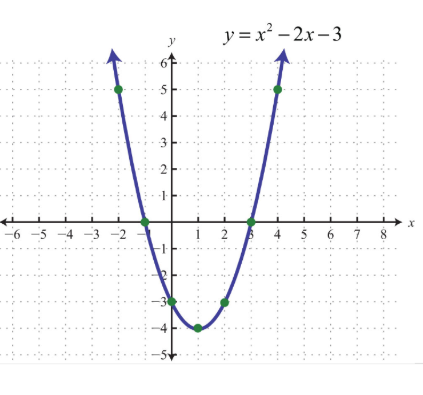
\includegraphics[width=0.7\linewidth]{parabolicfunction}
\end{figure}

We kunnen dit principe makkelijkst voorstellen aan de hand van een parabool. Deze wordt grafisch weergegeven op figuur \ref{fig:parabolicfunction}. Het minimum van deze parabolische functie wordt bereikt wanneer $x$ een waarde van 1 heeft. 
Als startpunt wordt een willekeurige waarde op de curve genomen waarbij dan nagegaan wordt in welke richting bewogen moet worden om dichter bij het minimum te komen. Wanneer het minimum gezocht wordt zou een stapgrootte gedefinieerd kunnen worden en dan telkens met even grote stappen afgedaald kunnen worden. Wanneer deze stapgrootte bepaald moet worden zou bij een kleine stapgrootte het minimum nauwkeuriger gedefinieerd zijn maar zou dit veel meer berekeningen vergen. Bij een grote stapgrootte zou het minimum snel berekend kunnen worden, maar het zou onnauwkeurig zijn. 

Bij gradient descent wordt deze stapgrootte dynamisch bepaald op basis van het product van de hellingsgraad en de learning rate, een vooraf bepaalde waarde die moet voorkomen dat de stapgrootte te groot wordt. Wanneer de hellingsgraad laag zal zijn betekent dit dat het minimum wordt benaderd en dus kleinere stappen genomen zullen worden om dit zo nauwkeurig mogelijk te bepalen. De kans dat 0 effectief wordt bereikt is zeer klein, daarom stopt het algoritme wanneer een vooraf bepaalde minimale stapgrootte wordt bereikt. Daarnaast kan ook een maximum aantal stappen ingesteld worden waarbij het algoritme stopt. 

Gradient descent kan duidelijk toegelicht worden aan de hand van deze 5 stappen, bij elke stap moet de waarde van de afgeleide opnieuw berekend worden:
\begin{enumerate}
    \item Neem de afgeleide van de verliesfunctie voor elke parameter in deze functie
    \item Kies willekeurige waarden voor deze parameters
    \item Voer de parameterwaarden in in de afgeleiden (in praktijk zal de gradi\"{e}nt numerisch bepaald worden)
    \item Bereken de stapgroottes: Stapgrootte = helling * learning rate 
    \item Bereken de nieuwe parameters: Nieuwe parameter = oude parameter - stapgrootte
\end{enumerate}

Herhaal stappen 3 tot 5 tot het minimum bereikt wordt.

Bij dit voorbeeld zou gewoon de afgeleide van deze parabool kunnen genomen worden om zo tot het minimum te komen, maar bij complexere functies is dit niet mogelijk en biedt gradient descent hiervoor een oplossing.

Bij gebruik van stochastic gradient descent wordt niet telkens alle data gebruikt wanneer de parameters herberekend worden, maar een willekeurige subset uit de dataset om het aantal berekeningen te reduceren wat deze methode performanter maakt zonder al te veel nauwkeurigheid te verliezen~\autocite{Starmer2019}.

Dan rest enkel Adam nog verklaard te worden. Dit is een variant op de klassieke vorm van gradient descent waarbij de learning rate aangepast voor elk gewicht binnen het netwerk en doorheen het trainingsproces.

Deze aanpassingen worden door de auteurs van Adam omschreven als het combineren van 2 andere uitbreidingen op gradient descent namelijk:

Adaptive Gradient Algorithm (AdaGrad) die er voor zorgt dat een per-parameter learning rate die performantie zal verbeteren van de gradi\"{e}nt.  

Root Mean Square Propagation (RMSProp)  deze uitbreiding op gradient descent zorgt voor aanpassingen in de learning rates op basis van de schaal van de laatste gradi\"{e}nten kortom hoe snel deze veranderen~\autocite{Brownlee2017}.


En zal geoptimaliseerd worden op basis van de 'mse' verliesfunctie. 
\captionof{listing}{Datavoorbereiding dataset ijsexpansie}
\label{}
\begin{minted}[
frame=lines,
framesep=2mm,
fontsize=\footnotesize,
linenos,breaklines
]{python}

# univariate lstm voorbeeld
from numpy import array
from keras.models import Sequential
from keras.layers import LSTM
from keras.layers import Dense

# Opslitsen van univariate sequentie in samples
def split_sequence(sequence, n_steps):
X, y = list(), list()
for i in range(len(sequence)):
# vinden van het einde van dit patroon
end_ix = i + n_steps
# nagaan of we ons na de sequentie bevinden
if end_ix > len(sequence)-1:
break
# verwerven van invoer en uitvoerdelen van het patroon
seq_x, seq_y = sequence[i:end_ix], sequence[end_ix]
X.append(seq_x)
y.append(seq_y)
return array(X), array(y)

# Bepalen van de sequentie
raw_seq = [10, 20, 30, 40, 50, 60, 70, 80, 90]

# bepalen van het aantal tijdsstappen
n_steps = 3

# onderverdelen in samples
X, y = split_sequence(raw_seq, n_steps)

# reshape from [samples, timesteps] into [samples, timesteps, features]
n_features = 1
X = X.reshape((X.shape[0], X.shape[1], n_features))

# definieer model
model = Sequential()
model.add(LSTM(50, activation='relu', input_shape=(n_steps, n_features)))
model.add(Dense(1))
model.compile(optimizer='adam', loss='mse')

# fit model
model.fit(X, y, epochs=200, verbose=0)

# demonstreer voorspelling
x_input = array([70, 80, 90])
x_input = x_input.reshape((1, n_steps, n_features))
yhat = model.predict(x_input, verbose=0)
print(yhat)
\end{minted}

\paragraph{\IfLanguageName{dutch}{Stacked LSTM}{Stacked LSTM}}

Een stacked LSTM is een variant op het Vanilla LSTM waarbij er meerdere LSTM lagen na elkaar geplaatst worden. Het toevoegen van een extra laag zal voor een langere uitvoeringstijd zorgen. Het voordeel hiervan is dat hierdoor meerdere onderdelen makkelijker geregistreerd kunnen worden en in verband met elkaar gebracht kunnen worden. Het stapelen van LSTM lagen zal ervoor zorgen dat deze lagen ook onderling uitvoerwaarden zullen uitwisselen die een sequentie van tijdsstappen zal beschrijven en niet gewoon 1 enkele tijdstap~\autocite{Brownlee2017b}.

\begin{figure}
    \centering
    \caption{Een stacked LSTM~\autocite{Brownlee2017b}}
    \label{fig:stacked_lstm}
    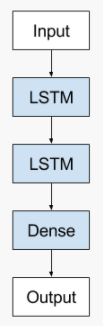
\includegraphics[width=0.15\linewidth]{stacked_lstm}
\end{figure}

\paragraph{\IfLanguageName{dutch}{Bidirectionele LSTM}{Bidirectional LSTM}}

Bidirectionele LSTMs kunnen getrained worden gebruik makend van alle beschikbare invoerinformatie uit het verleden en de toekomst binnen een specifieke tijdspanne. Dit door middel van de toestandsneuronen op te splitsen van een normaal Recurrent Neuraal Netwerk in een deel dat verantwoordelijk is voor de positieve tijdsdirectie en een deel voor de negatieve tijdsdirectie. ~\autocite{Brownlee2017a}

Bidirectionele LSTMs worden voornamelijk gebruikt bij language processing omdat de definitie van een woord afgeleid kan worden uit de context. De begrippen die bepalend zijn voor de definitie kunnen zich zowel voor als achter het woord zelf bevinden dus moet de zin vanuit 2 richtingen geanalyseerd kunnen worden om de definitie te achterhalen.

\begin{figure}
    \centering
    \caption{Weergave van een bidirectioneel LSTM model~\autocite{Colah2015}}
    \label{fig:bidirectional_lstm}
    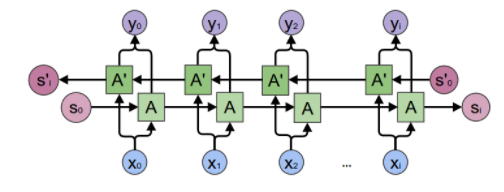
\includegraphics[width=0.7\linewidth]{bidirectional_lstm}
\end{figure}

\paragraph{\IfLanguageName{dutch}{CNN LSTM}{CNN LSTM}}

Een convolutioneel neuraal netwerk ook wel een CNN genoemd wordt voornamelijk gebruikt bij het analyseren van tweedimensionale grafische data. Een CNN is ook sterk in het extraheren en aanleren van features van eendimensionele data. Een CNN model kan ook gecombineerd worden met een LSTM model om een CNN-LSTM te vormen. Hierbij wordt het CNN gebruikt om subreeksen te interpreteren die op zich dan weer zullen ge\"{i}nterpreteerd worden als een reeks door het LSTM model. 

\paragraph{\IfLanguageName{dutch}{ConvLSTM}{ConvLSTM}}

ConvLSTM is ook een soort van CNN-LSTM waarbij het convolutionele deel rechtstreeks is ingebouwd binnen het LSTM gedeelte. Dus ook dit CNN-LSTM werd ontwikkeld voor het interpreteren van tweedimensionale grafische data maar kan aangepast worden voor gebruik bij univariabele tijdreeksvoorspellingen.

\begin{figure}
    \centering
    \caption{\textbf{(a)} Gewone LSTM cell, \textbf{(b)} Weergave van een ConvLSTM~\autocite{Rahman2019}}
    \label{fig:ConvLSTM}
    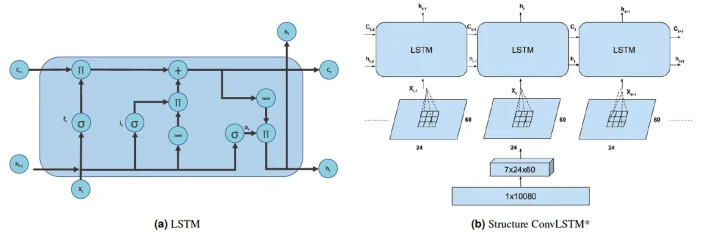
\includegraphics[width=0.7\linewidth]{ConvLSTM}
\end{figure}


\subsubsection{\IfLanguageName{dutch}{Multivariabele LSTM modellen}{Multivariate LSTM models}}

Bij multivariabele tijdreeksen zullen er in tegenstelling tot univariabele tijdsreeksen wel meerdere observaties zijn per tijdseenheid. Deze worden dan nog eens onderverdeeld in multiple input series en multiple parallel series. 

\paragraph{\IfLanguageName{dutch}{Meerdere invoerreeksen}{Multiple Input Series}}

Bij de variant met meerdere invoerreeksen zullen er meerdere invoerwaarden zijn voor elk tijdstip. Hierbij zal slechts voor 1 van de invoerreeksen een voorspelling gemaakt worden. 

\paragraph{\IfLanguageName{dutch}{Meerdere parallelle reeksen}{Multiple Parallel Series.}}
Bij de LSTM variant waarbij er meerdere parallelle reeksen zijn zullen er meerdere invoerwaarden zijn voor elk tijdstip. Hier zal er voor elke reeks een waarde voorspeld worden.


\subsubsection{\IfLanguageName{dutch}{Multi-Step LSTM modellen}{Multi-Step LSTM models}}

Tot nu toe werden enkel maar one-step LSTM modellen toegelicht waarbij de invoerreeks slechts zal resulteren in 1 uitvoerwaarde. Bij multi-step LSTM modellen zal er meer dan 1 uitvoerwaarde voorspeld worden.

\paragraph{\IfLanguageName{dutch}{Vector output model}{Vector output model}}

Bij dit type multi-step LSTM model zal de uitvoer onder de vorm van een vector weergegeven worden die de resultaten van de volgende tijdstappen zal weergeven en niet enkel van de volgende tijdstap. 

\paragraph{\IfLanguageName{dutch}{Encoder-Decoder Model}{Encoder-Decoder Model}}


Dit model is ontwikkeld om sequenties met variabele uitvoer te voorspellen~\autocite{Brownlee2017a}. Het is ook ontworpen om problemen waarbij er zowel invoer-als uitvoersequenties zijn te behandelen. Deze problemen worden ook wel benoemd als sequence-to-sequence of seq2seq-problemen. Deze techniek wordt voornamelijk gebruikt bij vertalingstoepassingen maar kan ook toegepast worden op tijdreeksen. 
Het model bestaat uit 2 hoofdonderdelen de encoder en de decoder. 

De encoder is verantwoordelijk voor het lezen en interpreteren van de invoerreeks. De encoder zal dan een vector met een vaste lengte uitvoeren die een interpretatie zal geven van de invoerreeks. Normaal zal de encoder een Vanilla LSTM model zijn, maar er kan even goed een stacked, bidirectioneel of CNN model gebruikt worden.

De decoder zal de uitvoer van de encoder dan gebruiken als invoer. Die zal dan voor elke tijdsstap een uitvoerwaarde zal geven. Deze uitvoer zal dan nog eens ge\"{i}nterpreteerd worden door een verborgen laag alvorens dit volledig model de multi-step uitvoerreeks zal teruggeven.

\begin{figure}
    \centering
    \caption{Encoder-Decoder Model~\autocite{Brownlee2017a}}
    \label{fig:encoder_decoder_lstm}
    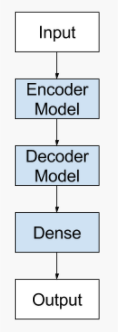
\includegraphics[width=0.15\linewidth]{encoder_decoder_lstm}
\end{figure}


\subsubsection{\IfLanguageName{dutch}{Multivariate Multi-Step LSTM Models LSTM modellen}{Multivariate Multi-Step LSTM Models LSTM models}}

\paragraph{\IfLanguageName{dutch}{Multiple input Multi-Step Output}{Multiple input Multi-Step Output}}

Wanneer men over een dataset beschikt met meerdere invoerparameters maar slechts 1 enkele parameter voor meerdere tijdsstappen dient te voorspellen spreekt men over multiple input multi-step output.

\paragraph{\IfLanguageName{dutch}{Multiple Parallel Input and Multi-Step Output}{Multiple Parallel Input and Multi-Step Output}}

Wanneer de dataset waarvan een voorspelling gemaakt moet worden meerdere invoerparameters heeft maar er  ook meerdere voorspeld moeten worden zal dit benoemd worden als een multiple parallel input and multi-step output LSTM.

\section{\IfLanguageName{dutch}{Prophet}{}}

Prophet is een procedure om tijdreeksen te voorspellen ontwikkeld door Facebook.~\autocite{Prophet2020} Deze procedure baseert zich op een additief model waar niet-lineaire trends gefit worden aan jaarlijkse, wekelijkse en dagelijkse seizoensgebondenheid hierbij zal ook rekening gehouden worden met zogenaamde ``holiday effects'', fluctuaties in de data die veroorzaakt worden door vakantieperiodes. Deze techniek zal best werken met tijdreeksen die een sterk seizoensgebonden effect hebben en waarvan ook meerdere seizoenen aan historische data beschikbaar zal zijn. Daarnaast houdt Prophet ook rekening met ontbrekende data, verschuivingen in de trend en zal het ook rekening houden met uitschieters. 

Het is eenvoudig om te gebruiken maar er zijn ook optimalisaties mogelijk indien men het model wil finetunen. Prophet is zowel beschikbaar in R als in Python



\section{\IfLanguageName{dutch}{Validatietechnieken}{}}

Om de kwaliteit van de modellen te beoordelen zal er telkens een deel van de dataset achtergehouden worden die niet zal gebruikt worden bij het opstellen van het model. Deze achtergehouden dataset wordt de testset genoemd. In het geval van een tijdreeks zullen dit altijd de laatste waarden zijn. Het model zal dan trachten deze laatste waarden te voorspellen waarna de voorspelde waarden vergeleken zullen worden met de waarden van de testset. Op basis hiervan kunnen we achterhalen hoe groot de fout is bij elk model, het model met de laagste fout zal dan de meest accurate voorspelling maken. 
In deze sectie zullen enkele verschillende methodes om de fout te berekenen toegelicht worden ~\autocite{Hyndman2018}.

\subsection{\IfLanguageName{dutch}{Foutmaten}{}}

\subsubsection{\IfLanguageName{dutch}{MAE}{}}
MAE staat voor mean absolute error. Deze zal berekend worden door het verschil te nemen tussen elke voorspelde tijdstap en de verwachte waarde voor deze tijdstap, hier de absolute waarde van te nemen en dan het gemiddelde te nemen van al deze absolute waarden. De formule voor de gemiddelde absolute fout wordt hieronder weergegeven.

\begin{equation}
MAE = \frac{\sum_{i=1}^{n} |y_i - \hat{y_i}|}{n}
\end{equation}

Dit is de meest eenvoudige foutmaat en wordt vaak gebruikt al moet er echter mee rekening gehouden worden dat deze fout eenheidsgebonden is en kan deze niet gebruikt worden om tijdreeksen te vergelijken die gebruik maken van andere eenheden. Dit heeft wel als voordeel dat deze fout makkelijk te interpreteren valt. Zo zou bijvoorbeeld een fout van 1 bij een tijdreeks over temperatuur in graden Celsius betekenen dat de gemiddelde fout bij het voorspellen van de temperatuur 1 graad Celsius is bij dat model.

\subsubsection{\IfLanguageName{dutch}{RMSE}{}}

RMSE staat voor root mean squared error. Deze wordt berekend door het verschil te nemen tussen tussen elke voorspelde tijdstap en de verwachte waarde bij deze tijdstap, dit te kwadrateren, het gemiddelde te nemen van deze kwadraten en dan de vierkantswortel te nemen van dit gemiddelde.
Dit kan ook als volgt geformuleerd worden:

\begin{equation}
RMSE = \sqrt{\frac{\sum_{i=1}^{n} (y_i - \hat{y_i})^2}{n}}
\end{equation}

Ook bij RMSE zal de eenheid gelijk blijven. Het verschil met MAE is echter dat een groot verschil tussen de voorspelde en effectieve waarde zwaarder zal doorwegen bij RMSE doordat deze eerst gekwadrateerd worden voordat het gemiddelde genomen wordt~\autocite{Kampakis2020}.

\subsubsection{\IfLanguageName{dutch}{MAPE \& RMSPE}{}}

MAPE staat voor mean absolute percentage error en RMSPE voor root mean square percentage error. Dit zijn procentuele fouten, dit type fout kan vergeleken worden tussen tijdreeksen met een verschillende eenheid. Dit zijn variaties op respectievelijk MAE en RMSE maar waarbij deler toegevoegd wordt bij het berekenen van het verschil tussen de voorspelde en de effectieve waarde. De formules van deze fouten worden hieronder weergegeven.

\begin{equation}
MAPE = \frac{\sum_{i=1}^{n} |\frac{y_i - \hat{y_i}}{y_i}|}{n}
\end{equation}

\begin{equation}
RMSPE = \sqrt{\frac{\sum_{i=1}^{n} (\frac{y_i - \hat{y_i}}{y_i})^2}{n}}
\end{equation}

\subsection{\IfLanguageName{dutch}{Cross-validation}{}}

Om een tijdreeks nog beter te benutten kan ook cross-validation gebruikt worden. Hierbij zal dezelfde tijdreeks meerdere malen gebruikt worden om het model te trainen, maar zal deze telkens uitgebreid worden zoals zichtbaar in figuur \ref{fig:parabolicfunction}. De accuraatheid van het model zal dan bepaald worden door de het gemiddelde te nemen van de accuraatheid voor elke opgestelde testset. Er moet echter rekening mee gehouden worden dat deze nieuwe training en testsets altijd nieuwe observaties moeten bevatten en de observaties van de trainingsset altijd moeten voorkomen voor deze van de bijhorende testset~\autocite{Shrivastava2020}.

\begin{figure}
    \centering
    \caption{Grafische weergave van de structuur van een cross-validation tijdreeks~\autocite{Hyndman2018} waarbij 1 tijdreeks zal opgedeeld worden in 20 train- en testreeksen}
    \label{fig:cross_validation_ts}
    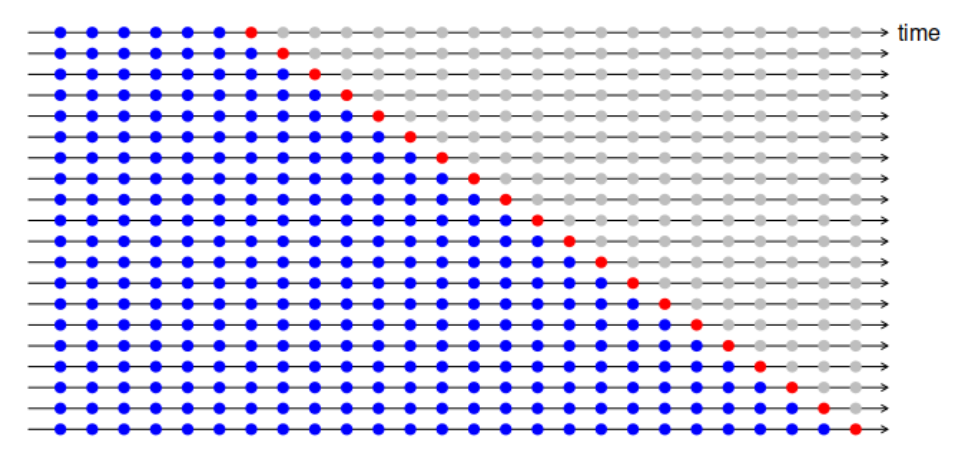
\includegraphics[width=0.9\linewidth]{cross_validation_ts}
\end{figure}



\chapter{\IfLanguageName{dutch}{Methodologie}{Methodology}}
\label{ch:methodologie}

Om te onderzoeken welke types modellen best presteren zal er voor elke combinatie van seizoensgebonden of niet-seizoensgebonden en univariate of multivariate data een notebook opgesteld worden. Op het einde van elke notebook zal dan aan elk model een foutscore toegekend zijn. Deze foutscore wordt bepaald door het gemiddelde te nemen van de mean average errors van elke partitie bij de datasetverdeling door cross-validation. Het model met de laagste foutscore zal de meest accurate voorspelling gemaakt hebben bij het type invoerdata bij dit deelprobleem voor de gebruikte data. 

Er dient echter vermeld te worden dat dit in zekere mate altijd zal afhangen van de invoerdata en dit type model niet noodzakelijk de beste prestatie zal leveren bij dit type invoerdata.

\section{Voorbereiding}
%\subsection{Benutte libraries}
\subsection{Datavoorbereiding}
\subsubsection{Dataset 1, temperatuur}
Hier zal het het deel van de dataset die de temperatuur weergeeft geformateerd worden  naar een dataset met 1 kolom en een index waarin de maand en het jaartal weergegeven worden van het jaar 1979 tot 2018.

\clearpage
\captionof{listing}{Datavoorbereiding dataset temperatuur}
\label{code:prep_temp}
\begin{minted}[
frame=lines,
framesep=2mm,
fontsize=\footnotesize,
linenos,breaklines
]{python}
# Source: https://www.kaggle.com/rainbowgirl/climate-data-toronto-19372018
tt = pd.read_csv('./data/Toronto_temp.csv')
tt = tt[tt['Day'] == 1]
tt['Year'] = tt['Year'].replace({'2,013':'2013',
'2,014':'2014',
'2,015':'2015',
'2,016':'2016',
'2,017':'2017',
'2,018':'2018'})
# tt.groupby('Year').count()
tt = tt[(tt['Year'] != '1937')]
ttt = tt.groupby('Year').count()
#ttt.head(50)
#tt.groupby('Year').count().tail(50)
meantt = tt.groupby('Year').mean()['Mean Temp (C)']
#meantt.index
#meantt
meantt.sort_index(inplace=True)

plt.xlabel('Years')
plt.ylabel('Temperature (C)')
plt.xticks(np.array(range(0,meantt.size,10)))
plt.scatter(meantt.index, meantt)

print('start : ' + meantt.index[0])
print('end : ' + meantt.index[-1])

new_row = pd.Series({'Mean Temp (C)' : 0.555556, 'Year': '2018', 'Month':12})
tt = tt.append(new_row, ignore_index=True)
tt['Year'] = tt['Year'].astype(int)
mean_temp_monthly = tt[['Year','Month','Mean Temp (C)']].set_index(['Year','Month']).sort_index()
# mean_temp_monthly
mean_temp_monthly = mean_temp_monthly[mean_temp_monthly.index.get_level_values(0).astype(int) >= 1979 ]
mean_temp_monthly
\end{minted}

Op listing \ref{code:prep_temp} wordt de code weergegeven de die ruwe dataset zal omzetten naar een dataset die bruikbaar zal zijn om te gebruiken voor deze bachelorproef. 


De delen die in commentaar staan geven een tussentijdse weergave van de dataset, maar worden niet telkens weergegeven om het aantal tabellen binnen deze sectie overzichtelijk te houden. \\


Zo wordt op lijn 2 het originele csv-bestand ingelezen deze ruwe data zal er uit zien als deze zichtbaar op figuur \ref{fig:tempdatagraph}. \\
Op lijn 3 worden enkel de waarden van de eerste dag van de maand behouden in de dataset \\
Daarna worden van lijn 4 tot lijn 9 de jaartallen aangepast zodat deze overeenkomen met de rest van de dataset. \\
Op lijn 10 wordt het aantal rijen per jaar weergegeven. \\
Op lijn 11 zal het eerste jaar uit de dataset verwijderd worden aangezien deze data onvolledig is. \\
Op lijn 12 wordt het aantal jaren toegekend aan de variabele $ttt$ \\
Op lijn 15 wordt het gemiddelde van de temperaturen van de eerste dagen van de maand per jaar berekend. \\
Op lijn 18 wordt dit gemiddelde gesorteerd. \\



\begin{figure}
    \centering
    \caption{Ruwe invoerdata}
    \label{fig:tempdataraw.png}
    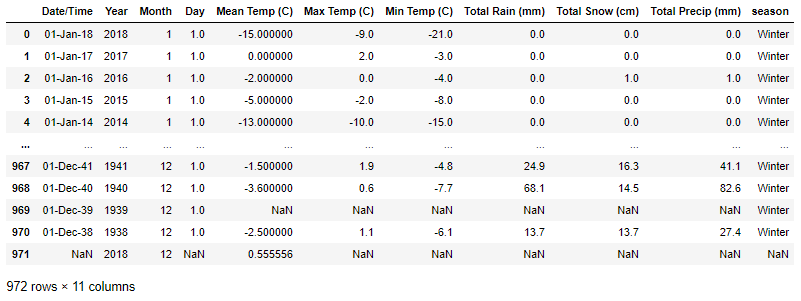
\includegraphics[width=1\linewidth]{temp_data_rawpng}
\end{figure}


Van lijn 20 tot lijn 23 worden de labels en ijkingen gedefini\"{e}erd van de grafiek die de data zal weergeven en zichtbaar is op figuur \ref{fig:tempdatagraph} die op lijn 24 getekend zal worden. \\



\begin{figure}
    \caption{Grafische weergave jaarlijkse temperatuur}
    \label{fig:tempdatagraph}
    \centering
    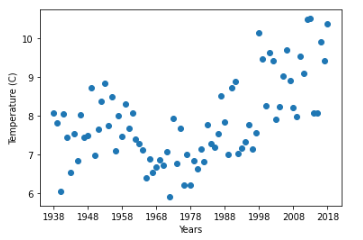
\includegraphics[width=0.7\linewidth]{temp_data_graph}
\end{figure}

Op lijn 25 en 26 worden de start en de eindjaren van deze dataset afgeprint om ze te kunnen vergelijken met de start en de eindjaren van de andere dataset.

Op lijn 28 wordt de laatste waarde voor het jaar 2018 toegevoegd aangezien deze nog niet in de dataset zat. \\
Op lijn 29 wordt deze nieuwe waarde toegevoegd.\\

Op lijn 30 wordt de waarde voor het jaar geconverteerd naar een integer. \\
Op lijn 31 wordt de dataset geindexeerd op jaar en maand. \\
Op lijn 33 worden de jaren die voor 1979 komen uit de dataset gefilterd omdat de waarden voor de andere dataset starten vanaf 1979.\\
Op lijn 34 wordt het resultaat van de dataformattering uitgevoerd zichtbaar op figuur \ref{fig:tempdata}.




\begin{figure}
    \centering
    \caption{Resultaat van data formatting}
    \label{fig:tempdata}
    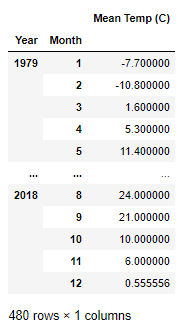
\includegraphics[width=0.3\linewidth]{temp_data}
\end{figure}



\clearpage



\subsubsection{Dataset 2, ijsdikte}

Hier zal het deel van de dataset die de ijsdikte weergeeft geformateerd worden naar een dataset met 1 kolom en het jaartal van het jaar 1979 tot 2018 als index zal dienen.

\captionof{listing}{Datavoorbereiding dataset temperatuur}
\label{code:prep_ice}
\begin{minted}[
frame=lines,
framesep=2mm,
fontsize=\footnotesize,
linenos,breaklines
]{python}
#source: https://nsidc.org/arcticseaicenews/sea-ice-tools/
ice2 = pd.read_csv('./data/seaice2.csv')
# ice2
ice2_mean = ice2.mean()[1:-2]
# ice2_mean
ice2_mean.index = ice2_mean.index.values.astype(int)

plt.title('Yearly ice extent')
plt.scatter(ice2_mean.index,ice2_mean)
plt.xlabel('Years')
plt.ylabel('Extent')
plt.show()

# ice2['2018']
# pd.concat([ice2['2016'],ice2['2017'],ice2['2018'],ice2['2019']]).reset_index()[0]
# ice2[['2018']].append(ice2[['2019']])
ice2.rename(columns={'Unnamed: 0' : 'Month', 'Unnamed: 1' : 'Day'}, inplace = True)
ice2.drop([' ','1981-2010','Day','1978','2020'],axis=1,inplace=True)
values = ice2.values
i = 0
for row in values :
    if type(row[0]) != str :
        values[i][0] = month
    else:
        month = row[0]
    i = i +1
# ice2.columns.values
ice2_clean = pd.DataFrame(values)
ice2_clean.columns = ice2.columns.values
# ice2_clean.head(5)
ice2_monthly_mean = ice2_clean.set_index('Month').astype(float).groupby('Month',sort=False).mean()
# ice2_monthly_mean
# ice2_monthly_mean.T.stack().index.get_level_values(0)
# ice2_monthly_mean.T.stack().reset_index(level=['Month']).drop(columns=['Month'])
ice2_monthly_mean_chron = ice2_monthly_mean.T.stack().reset_index(level=['Month']).drop(columns=['Month'])
# ice2.columns.size
plt.title('Monthly ice extent')
plt.plot(ice2_monthly_mean_chron.values)
plt.xticks(np.array(range(0,500,75)))
plt.xlabel('Cumulative month')
plt.ylabel('Extent')
plt.show()

# np.unique(ice2_monthly_mean_chron.index.values).size*12
print('from ' + ice2_monthly_mean_chron.index.values[0] + ' until ' + ice2_monthly_mean_chron.index.values[-1])
ice2_monthly_mean_chron = ice2_monthly_mean.T.stack().reset_index(level=['Month']).drop(columns=['Month'])
ice2_monthly_mean_chron.columns = ['ice_extent']
ice2_monthly_mean_chron
\end{minted}

Op lijn 2 zal de ijsdataset ingelezen worden en zal er uitzien zoals zichtbaar op figuur \ref{fig:icedataraw} \\
Op lijn 4 zal het gemiddelde genomen worden van alle kolommen tussen eerste en de voorlaatste. De eerste, de voorlaatste en de laatste kolom worden uit de dataset gelaten omdat deze irrelevant zijn voor dit onderzoek. \\
Op lijn 6 worden de indexwaarden geconverteerd naar integers. \\

\begin{figure}
    \centering
    \caption{Ruwe data van de jaarlijkse ijsdiktes}
    \label{fig:icedataraw}
    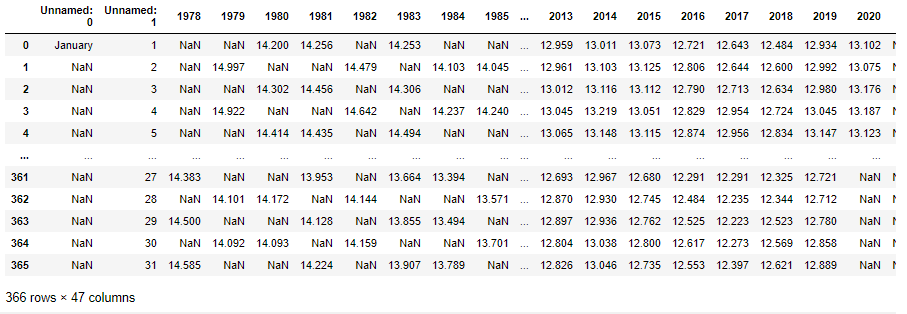
\includegraphics[width=1\linewidth]{ice_data_rawpng}
\end{figure}

De code van lijn 8 tot lijn 12 zal ervoor zorgen dat de jaarlijkse data grafisch weergegeven wordt. \\
Op lijn 17 zullen de kolomnamen hernoemd worden en op lijn 18 worden de overbodige kolommen verwijderd. \\

De code van lijn 18 tot lijn 26 zal er voor zorgen dat de maandkolom aangevuld wordt omdat deze tot hiertoe nog onvolledig zal zijn. \\
Op lijn 28 wordt een nieuwe dataframe ge\"{i}nitialiseerd waarvan de kolommen op lijn 29 aangevuld worden. \\
Op lijn 31 wordt hier het maandelijks gemiddelde genomen van deze nieuwe dataframe en opgeslaan in de variabele en op lijn 35 worden deze in chronologische volgorde geplaatst.\\

Het deel code van lijn 37 tot en met lijn 42 zal zorgen voor de grafische weergave van de maandelijkse ijsdikte weergegeven op figuur\ref{fig:iceextentmonthly}. \\

\begin{figure}
    \centering
    \caption{Grafische weergave van de maandelijkse ijsdiktes}
    \label{fig:iceextentmonthly}
    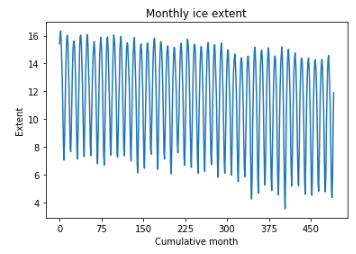
\includegraphics[width=0.7\linewidth]{ice_extent_monthly}
\end{figure}

Op lijn 45 worden de start en eindjaartallen uitgeprint. \\
De code op lijn 46 zal ervoor zorgen dat de maandindex verwijderd wordt.\\
Op lijn 47 zal de kolom hernoemd worden en op lijn 48 zal het resultaat uitgeprint worden, dit zal er uit zien zoals zichtbaar op figuur\ref{fig:iceextentdata}.

\begin{figure}
    \centering
    \caption{Data van de maandelijks ijsdiktes}
    \label{fig:iceextentdata}
    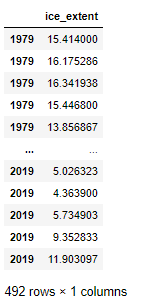
\includegraphics[width=0.3\linewidth]{ice_extent_data}
\end{figure}

\subsubsection{Combineren van de datasets}

In dit deel van de datavoorbereiding zullen de datasets gecombineerd worden.

\captionof{listing}{Datavoorbereiding dataset temperatuur}
\begin{minted}[
frame=lines,
framesep=2mm,
fontsize=\footnotesize,
linenos,breaklines
]{python}
ice2_monthly_mean_chron_cut = ice2_monthly_mean_chron[:-12]
# ice2_monthly_mean_chron
# ice2_monthly_mean_chron_cut
# mean_temp_monthly
# ice2_monthly_mean_chron_cut
combined = mean_temp_monthly[mean_temp_monthly.index.get_level_values(0) >= 1979]
combined['ice_extent'] = ice2_monthly_mean_chron_cut.values
# combined
combined.rename(columns={'Mean Temp (C)': 'mean_temp'}, inplace=True)
dataframe_monthly = combined
# dataframe_monthly
# dataframe_monthly[['mean_temp']]
plt.plot(dataframe_monthly[['mean_temp']].values[-24:],label='temperature')
plt.plot(dataframe_monthly[['ice_extent']].values[-24:],label='ice extent')
plt.legend()
plt.show()
dataframe_yearly = combined.groupby('Year').mean()
# dataframe_yearly
# dataframe_monthly[['mean_temp']].values
plt.plot(dataframe_monthly[['mean_temp']].values,label='temperature')
plt.plot(dataframe_monthly[['ice_extent']].values,label='ice extent')
plt.legend()
dataframe_monthly.to_csv('./data/dataframe_monthly.csv')
dataframe_yearly.to_csv('./data/dataframe_yearly.csv')
\end{minted}

Op lijn 1 worden de laatste 12 waarden van de gemiddelde maandelijkse chronologische dataset in een nieuwe variabele gestoken. \\
Op lijn 6 wordt een nieuwe dataset ge\"{i}nitialiseerd waar de maandelijkse gemiddelde temperaturen van 1979 ingevoerd worden.\\
Op lijn 7 worden de ijsdiktes hieraan toegevoegd. \\
Op lijn 9 wordt de kolom hernoemd op de lijn erna wordt de dataset nog eens toegevoegd aan een duidelijkere variabelenaam. \\

De code op lijn 13 tot 17 zorgt voor de grafische weergave van de gecombineerde dataset van de laatste 2 jaren weergegeven op figuur\ref{fig:combinedlastyears}. Hier valt op te merken dat de ijsdikte zal vergroten wanneer de temperatuur laag is. Dit is logisch aangezien het ijs zal smelten bij hogere temperaturen. \\

\begin{figure}
    \centering
    \caption{Grafische weergave van de ijsdikte en de temperatuur van de laatste 2 jaar}
    \label{fig:combinedlastyears}
    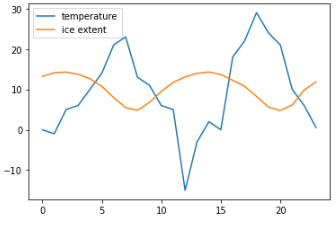
\includegraphics[width=0.7\linewidth]{combined_last_years.PNG}
\end{figure}

De code op lijn 17 zal het jaarlijks gemiddelde nemen.

Op lijn 20 tot 23 wordt de code weergegeven die ervoor zal zorgen dat het volledige maandelijks gemiddelde weergegeven zal worden van 1979 tot 2018. Dit valt te beschouwen op figuur \ref{fig:combinedlastyears}. Hierop kan vastgesteld worden dat de temperatuur lichtjes zal dalen terwijl de ijsdikte zal stijgen.

\begin{figure}
    \centering
    \caption{Grafische weergave van de ijsdikte en de temperatuur}
    \label{fig:combinedmonths}
    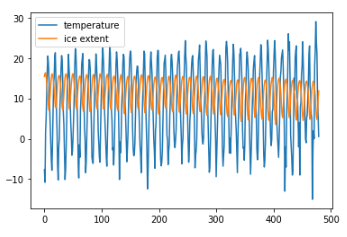
\includegraphics[width=0.7\linewidth]{combined_months.PNG}
\end{figure}

Op lijn 23 en 24 worden de dataframes weggeschreven naar csv-bestanden zodat ze kunnen gebruikt worden bij het opstellen van de modellen.


\section{Univariate niet-seizoensgebonden}

In dit deel zullen de voorspellingsmodellen voor univariate niet-seizoensgebonden data opgesteld worden. De modeltypes die bekeken zullen worden zijn ARIMA, LSTM en Prophet. Om dit te onderzoeken zullen er voorspellingen gemaakt worden van de gemiddelde jaarlijkse temperatuur.

\subsection{Algemene methodes}

Hier worden enkele algemene methodes gedefinieerd namelijk de full\textunderscore graph methode die een grafiek zal weergeven van de ingevoerde gedifferentieerde tijdreeks die ook als invoerparameter gebruikt zal worden samen met de grafiektitel.

Daarnaast wordt ook nog de methode revert\textunderscore diff gedefinieerd waar de gediferentieerde voorspellingen terug omgezet worden naar voorspellingen in miljoenen vierkante kilometers. Hiervoor zijn de gedifferentieerde voorspellingen en de originele dataset nodig als invoerparameters.

\captionof{listing}{Opstellen van algemene methodes}
\begin{minted}[
frame=lines,
framesep=2mm,
fontsize=\footnotesize,
linenos,breaklines
]{python}

# define functions used troughout the notebook

# define function for plotting last prediction and the actual data
def full_graph(predicted_diff, title):

# format predictions by adding NaN values in front
predictionsArray = np.asarray(revert_diff(predicted_diff, ts))
zerosArray = np.zeros(ts.values.size-len(predictionsArray.flatten()))
cleanPrediction = pd.Series(np.concatenate((zerosArray,predictionsArray))).replace(0,np.NaN)
cleanPrediction.index = ts.index.values

# plot
plt.title(title)
plt.plot(ts, marker='o', color='blue',label='Actual values')
plt.plot(cleanPrediction, marker='o', color='red',label='Last 4 year prediction')
plt.ylim([0,15])
plt.legend()

plt.show()

# define function for reverting a differenced dataset
def revert_diff(predicted_diff, og_data):

# retrieve last value
last_value = og_data.iloc[-predicted_diff.size-1][0]

# initialize reverted array
predicted_actual = np.array([])

# add each value in the differenced array with the last actual value
for value_diff in predicted_diff:
actual_value = last_value + value_diff
predicted_actual = np.append(predicted_actual, actual_value)
last_value = actual_value

return predicted_actual
\end{minted}

\subsection{Stationariteit}

Dan zal nagegaan worden in hoeverre deze dataset stationair is met gebruik van de hieronder omschreven test\textunderscore stationarity methode. Dit is noodzakelijk voor het opstellen van het ARIMA model.

\captionof{listing}{Test stationarity}
\begin{minted}[
frame=lines,
framesep=2mm,
fontsize=\footnotesize,
linenos,breaklines
]{python}
# define method to visualise the stationarity of a time series
def test_stationarity(timeseries):

    #Determing rolling statistics
    rolmean = timeseries.rolling(12).mean()
    rolstd = timeseries.rolling(12).std()
    
    #Plot rolling statistics:
    orig = plt.plot(timeseries, color='blue',label='Original')
    mean = plt.plot(rolmean, color='red', label='Rolling Mean')
    std = plt.plot(rolstd, color='black', label = 'Rolling Std')
    plt.legend(loc='best')
    plt.title('Rolling Mean & Standard Deviation')
    plt.show(block=False)

# check stationarity of time serie
test_stationarity(ts)
\end{minted}

Het resultaat van de test\textunderscore stationarity methode wordt weergegeven op figuur \ref{fig:stationarityunivariatenonseasonal}. Daar kan opgemerkt worden dat de data niet stationair is maar er een dalende trend aanwezig is.

\begin{figure}
    \centering
    \caption{Resultaat test stationarity}
    \label{fig:stationarityunivariatenonseasonal}
    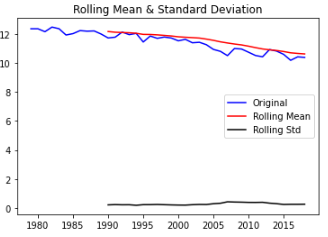
\includegraphics[width=0.7\linewidth]{stationarity_univariate_non_seasonal}
\end{figure}

Om deze trend te neutraliseren en de data stationair te maken zal het random walk difference genomen worden en nogmaals de stationariteit testen.

\captionof{listing}{Test stationarity bij random walk differencing}
\begin{minted}[
frame=lines,
framesep=2mm,
fontsize=\footnotesize,
linenos,breaklines
]{python}
# take the random walk difference of the time serie
ts_diff = ts - ts.shift(1)
ts_diff = ts_diff.dropna()

# display stationarity of the newly differenced time serie
test_stationarity(ts_diff)
\end{minted}

Door hiervan nogmaals de stationariteit te testen wordt figuur\ref{fig:stationarityunivariatenonseasonal2} bekomen. Hierop valt af te lezen dat de data nu wel stationair is.

\begin{figure}
    \centering
    \caption{Resultaat test stationarity na random walk differencing}
    \label{fig:stationarityunivariatenonseasonal2}
    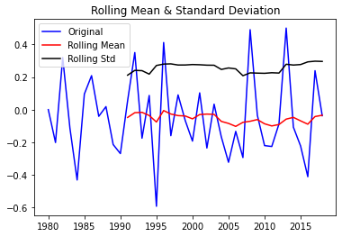
\includegraphics[width=0.7\linewidth]{stationarity_univariate_non_seasonal2}
\end{figure}

\subsection{Cross validation}

Om aan cross validation te doen moet de tijdreeks opgesplitst worden in verschillende reeksen waarbij de testset van de vorige reeks telkens toegevoegd wordt aan de trainingsset van de huidige reeks. Bij de univariate niet-seizoensgebonden tijdreeks wordt telkens een testgrootte van 4 genomen. De waarden worden ook enkel uitgeprint indien de testset groter is dan 20 om een minimale testset te garanderen. De grootte van de train-en testset zal ook geprint worden bij het uitvoeren van dit stuk code.

\captionof{listing}{Code voor het opstellen van cross-validation}
\begin{minted}[
frame=lines,
framesep=2mm,
fontsize=\footnotesize,
linenos,breaklines
]{python}
# initialize TimeSeriesSplit object
tscv = TimeSeriesSplit(n_splits = 8)

# loop trough all split time series that have a trainingsset with more than 20 values
for train_index, test_index in tscv.split(ts_diff):
    if train_index.size > 20:

        # initialize cross validation train and test sets
        cv_train, cv_test = ts_diff.iloc[train_index], ts_diff.iloc[test_index]
        
        # visiualize cross_validation structure for reference
        print("TRAIN:", train_index.size)
        print("TEST:", test_index.size)
        print()
\end{minted}

\subsection{ARIMA}

In dit stuk code worden de hyperparameters bepaald die de beste resultaten zullen behalen. Zo worden alle mogelijke parametercombinaties binnen het ARIMA model getest op de data met cross validation. De best presterende parameters die dus zorgen voor de laagste MAE score worden behouden en zullen gebruikt worden voor de finale voorspelling.

\captionof{listing}{Bepalen van de hyperparameters}
\begin{minted}[
frame=lines,
framesep=2mm,
fontsize=\footnotesize,
linenos,breaklines
]{python}
%%time
# ARIMA
from statsmodels.tsa.arima_model import ARIMA
import itertools
import warnings
import sys
from sklearn.metrics import mean_absolute_error

# Define the p, d and q parameters to take any value between 0 and 2
p = q = range(0, 5)
d = range(0,3)

# Generate all different combinations of p, q and q triplets
pdq = list(itertools.product(p, d, q))

# initialize variables
best_pdq = pdq
best_mean_mae = np.inf

# specify to ignore warning messages to reduce visual clutter
warnings.filterwarnings("ignore") 

# loop trough all possible parameter combinations of pdq
for param in pdq:
    print(param)
    
    # some parametercombinations might lead to crash, so catch exceptions and continue
    try:  
        
        # initialize the array which will contain the mean average errors
        maes = []
        
        # loop trough all split time series that have a trainingsset with more than 20 values
        for train_index, test_index in tscv.split(ts_diff):
            if train_index.size > 20:
            
                # initialize cross validation train and test sets
                cv_train, cv_test = ts_diff.iloc[train_index], ts_diff.iloc[test_index]
                
                # build model
                model = ARIMA(cv_train, order=(param))
                
                # fit model
                model_fit = model.fit()
                
                # make predictions
                predictions =  model_fit.predict(start=len(cv_train), end=len(cv_train)+cv_test.size-1, dynamic=False)
                
                # renaming for clarity
                prediction_values = predictions.values
                true_values = cv_test.values
                
                # error calculation this part of the cross validation
                maes.append(mean_absolute_error(true_values, prediction_values))
            
        
        # error calculation for this parameter combination
        mean_mae = np.mean(maes)
        print('MAE: ' + str(mean_mae))    
        
        # store parameters resulting in the lowest mean MAE
        if mean_mae < best_mean_mae:
            best_mean_mae = mean_mae
            best_maes = maes
            best_pdq = param
            best_predictions = prediction_values
            
    except Exception as e:
    print(e)
    continue

# logging
print()
print('Best MAE = ' + str(best_mean_mae))
print(best_pdq)
\end{minted}

Hieruit blijkt dat de beste parametercombinatie voor een bereik van 0 tot 5 voor de $p$ en $q$ waarden en 0 tot 2 voor de $d$ waarden (3,0,0) zijn. De $d$ waarden blijven zo beperkt omdat een waarde hoger dan 1 in praktijk niet voorkomt zoals beschreven in de literatuurstudie. Dit zijn dan ook de parameterwaarden die gebruikt zullen worden voor de finale iteratie van ARIMA. Een hoger bereik zou tot een beter resultaat kunnen leiden maar ook tot overfitting en zal zeker zorgen voor een hogere uitvoeringstijd omwille van deze redenen is het bereik van $p$ en $q$ beperkt tot 5.

\captionof{listing}{Finale iteratie ARIMA}
\begin{minted}[
frame=lines,
framesep=2mm,
fontsize=\footnotesize,
linenos,breaklines
]{python}
start_time = timeit.default_timer()

# specify to ignore warning messages
warnings.filterwarnings("ignore") 

print("----")

# initialize the array which will contain the mean average errors
maes = []

# loop trough all split time series that have a trainingsset with more than 20 values
for train_index, test_index in tscv.split(ts_diff):
    if train_index.size > 20:
    
        # initialize cross validation train and test sets
        cv_train, cv_test = ts_diff.iloc[train_index], ts_diff.iloc[test_index]
        
        # build model
        arima = ARIMA(cv_train, best_pdq).fit(start_ar_lags=1,disp=False)
        
        # make predictions
        predictions = arima.forecast(steps=4)
        prediction_values = predictions[0]
        true_values = cv_test.values
        
        # error calc
        maes.append(mean_absolute_error(true_values, prediction_values))
        
        # last actual prediction 
        last_prediction_ARIMA = prediction_values
        
        print("I",end="")

# store results to variables
time_ARIMA = timeit.default_timer() - start_time
mae_mean = np.mean(maes)
MAE_ARIMA = mae_mean
last_MAE_ARIMA = maes[-1]

# logging
print()
print('Mean MAE: %.3f x 1 000 000 km\u00b2' % MAE_ARIMA)
print('MAE of last prediction: %.3f x 1 000 000 km\u00b2' % last_MAE_ARIMA)
print('Execution time: %.3f seconds' % time_ARIMA)
full_graph(last_prediction_ARIMA, 'Last prediction ARIMA')
print('Mean average errors:')
print(maes)
\end{minted}

De bovenstaande code zal leiden tot de uitvoer die zichtbaar is op figuur\ref{fig:uvnsarima}. Hier wordt de gemiddelde MAE overheen de verschillende iteraties bij cross validation weergeven alsook de MAE van de laatste voorspelling. Daarnaast wordt ook de uitvoeringstijd weergegeven en ook de voorspelde waarden van de laatste partitie van de cross validation ten opzichte van de originele waarden. Ook de reeks met de MAEs wordt weergegeven.

\begin{figure}
    \centering
    \caption{Resultaat finale iteratie ARIMA}
    \label{fig:uvnsarima}
    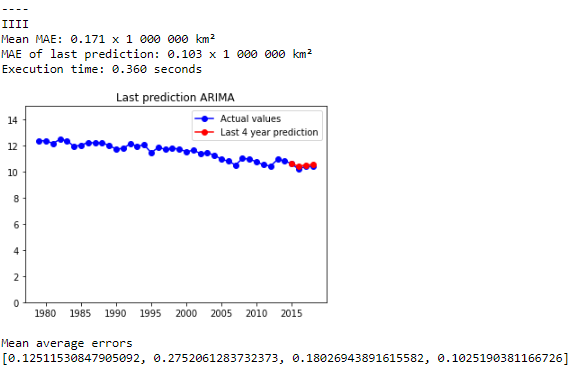
\includegraphics[width=1\linewidth]{uv_ns_ARIMA}
\end{figure}

\clearpage
\subsection{LSTM}

Het volgende model dat getest zal worden is een LSTM model. Aangezien dit een neuraal netwerk is zijn er op voorhand enkele methodes gedefinieerd om het overzicht te bewaren. 

De eerste methode die gedefinieerd wordt is de split\textunderscore sequence dit zal er voor zorgen dat de univariabele tijdreeks opgesplitst wordt in samples zodat deze gebruikt kunnen worden als invoerwaarden voor een LSTM netwerk. De originele tijdreeks dient ingegeven te worden bij sequence, het aantal invoerstappen en het aantal uitvoerstappen dienen ook meegegeven te worden.

Daarnaast wordt ook de methode build\textunderscore model gedefinieerd die het model zal opstellen. Dit zal gebeuren door de structuur van het LSTM model op te stellen met gebruik van het aantal features, het aantal neuronen in de LSTM laag, de dropout rate en de batchgrootte deze parameters diennen ook ingegeven te worden. Na het opstellen van het model zal het gefit worden aan de trainingsdata.

Ten slotte wordt ook nog de functie predict opgesteld. Deze functie verwacht de trainingsset, het model en het aantal features als invoerwaarde en zal het verdere verloop van de tijdreeks trachten te voorspellen. 

\captionof{listing}{Functies voor het opstellen van een LSTM model}
\begin{minted}[
frame=lines,
framesep=2mm,
fontsize=\footnotesize,
linenos,breaklines
]{python}
from keras.layers import Dropout
# split a univariate sequence into samples
def split_sequence(sequence, n_steps_in, n_steps_out):
    X, y = list(), list()
    for i in range(len(sequence)):
        # find the end of this pattern
        end_ix = i + n_steps_in
        out_end_ix = end_ix + n_steps_out
        
        # check if we are beyond the sequence
        if out_end_ix > len(sequence):
        break
        
        # gather input and output parts of the pattern
        seq_x, seq_y = sequence[i:end_ix], sequence[end_ix:out_end_ix]
        X.append(seq_x)
        y.append(seq_y)
    return array(X), array(y)

def build_model(raw_seq, n_steps_in, n_steps_out, n_features, n_neurons, dropout, batch_s):

    # split into samples
    X, y = split_sequence(raw_seq.values.flatten(), n_steps_in, n_steps_out)
    
    # reshape from [samples, timesteps] into [samples, timesteps, features]
    X = X.reshape((X.shape[0], X.shape[1], n_features))
    
    # define model
    model = Sequential()
    model.add(LSTM(n_neurons, activation='relu'))
    model.add(Dropout(dropout))
    model.add(Dense(n_steps_out))
    model.compile(optimizer='adam', loss='mae')
    
    # fit model
    model.fit(X, y, batch_size=batch_s, epochs=100, verbose=0)
    
    return model


def predict(x_input, model, n_features):
    n_features = 1
    
    # reshape data
    x_input = x_input.reshape((1, n_steps_in, n_features))
    
    # predict
    yhat = model.predict(x_input, verbose=0)
    
    return yhat
\end{minted}

Ook bij LSTM dienen de hyperparameters geoptimaliseerd te worden. Dit gebeurt door middel van onderstaande code. Waarbij een reeks mogelijk waarden gedefinieerd wordt op lijn 15 tot 18 waarvan alle mogelijk combinaties getest worden en waarvan de best presterende combinatie bijgehouden wordt.

\captionof{listing}{Bepalen van de hyperparameters}
\begin{minted}[
frame=lines,
framesep=2mm,
fontsize=\footnotesize,
linenos,breaklines
]{python}
%%time

# Disabled tf warning because of visual clutter
tf.compat.v1.logging.set_verbosity(tf.compat.v1.logging.ERROR)


# constant variables
n_steps_in = 4
n_steps_out = 4
n_features  = 1
maes = []
global_maes = []

# optimizable variables
n_neurons_array = [1,10,20]
dropout_array = [0,0.5,0.99]
batch_size_array = [1,8]


# initialize values
best_MAE = 100
best_n_neurons = 0
best_activation = 'none'
best_dropout = 0
best_batch_size = 0

# loop over all possible parameter combinations
for n_neurons in n_neurons_array:
    for dropout in dropout_array:
        for batch_size in batch_size_array:
        
            print("----")
            
            # loop trough all split time series that have a trainingsset with more than 20 values
            for train_index, test_index in tscv.split(ts_diff): 
                if train_index.size > 20:  
                
                    # initialize cross validation train and test sets
                    y_train, y_test = ts_diff.iloc[train_index], ts_diff.iloc[test_index]
                    
                    # build model
                    lstm_model = build_model(y_train, n_steps_in, n_steps_out, n_features, n_neurons, dropout, batch_size)
                    
                    # make predictions
                    x_input = array(y_test)
                    y_predicted = predict(x_input, lstm_model, n_features).flatten()
                    y_actual = y_test.values
                    
                    # error calculation this part of the cross validation
                    maes.append(mean_absolute_error(y_actual, y_predicted))
                    
                    print("I",end="")
                    
                    # last actual prediction 
                    last_prediction_LSTM = y_predicted
                    
            # error calculation for this parameter combination
            MAE_LSTM = np.mean(maes)
            last_MAE_LSTM = maes[-1]
            global_maes.append(MAE_LSTM)
            
            # store parameters resulting in the lowest mean MAE
            if best_MAE > MAE_LSTM:
                best_n_neurons = n_neurons
                best_dropout = dropout
                best_batch_size = batch_size
                best_MAE = MAE_LSTM
            
            # log values for parameter combination
            print()
            print(n_neurons)
            print(dropout)
            print(batch_size)
            print(MAE_LSTM)
            print()    

# log parameter combination with best result
print('Best:')
print('N neurons')
print(best_n_neurons)
print('Dropout rate')
print(best_dropout)
print('Batch size')
print(best_batch_size)
print('MAE')
print(best_MAE)
plt.bar(range(0,len(global_maes)), global_maes)
\end{minted}

Na het uitvoeren van deze code blijkt er nauwelijks verschil te zijn bij het aanpassen van de hyperparameters. Dit valt af te leiden uit de MAE's die weergegeven worden door de plot op lijn 87. Die figuur\ref{fig:uvnslstmbar} als resultaat zal hebben.
Dit blijkt ook wanneer deze code meerdere malen doorlopen wordt aangezien er verschillende resultaten bekomen worden.

\begin{figure}
    \centering
    \caption{Grafische weergave verschil in MAE's bij verschillende hyperparameters met MAE op de y-as}
    \label{fig:uvnslstmbar}
    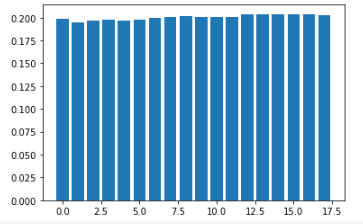
\includegraphics[width=1\linewidth]{uv_ns_LSTM_bar}
\end{figure}

Om verder te gaan zullen de waarden 1 voor het aantal neuronen gebruikt worden, 0 voor de beste dropout rate en 8 voor de batch size. 

\captionof{listing}{Finale iteratie LSTM}
\begin{minted}[
frame=lines,
framesep=2mm,
fontsize=\footnotesize,
linenos,breaklines
]{python}

%%time

start_time = timeit.default_timer()

# Disabled tf warning because of visual clutter
tf.compat.v1.logging.set_verbosity(tf.compat.v1.logging.ERROR)


# constant variables
n_steps_in = 4
n_steps_out = 4
n_features  = 1
maes = []


# optimizable variables
n_neurons = best_n_neurons
dropout = best_dropout
batch_s = best_batch_s

print("----")

# loop trough all split time series that have a trainingsset with more than 20 values
for train_index, test_index in tscv.split(ts_diff):
    if train_index.size > 20:  
        # initialize cross validation train and test sets
        y_train, y_test = ts_diff.iloc[train_index], ts_diff.iloc[test_index]
        
        # build model
        lstm_model = build_model(y_train, n_steps_in, n_steps_out, n_features, n_neurons, dropout, batch_s)
        
        # make predictions
        x_input = array(y_test)
        y_predicted = predict(x_input, lstm_model, n_features).flatten()
        y_actual = y_test.values
        
        # error calc
        maes.append(mean_absolute_error(y_actual, y_predicted))
        
        print("I",end="")
    
# last actual prediction 
last_prediction_LSTM = y_predicted

# store variables
time_LSTM = timeit.default_timer() - start_time
MAE_LSTM = np.mean(maes)
last_MAE_LSTM = maes[-1]

# visualisation
print()
print('Mean MAE: %.3f x 1 000 000 km\u00b2' % MAE_LSTM)
print('MAE of last prediction: %.3f x 1 000 000 km\u00b2' % last_MAE_LSTM)
print('Execution time: %.3f seconds' % time_LSTM)
full_graph(last_prediction_LSTM, 'Last prediction LSTM')
print('Mean average errors')
print(maes)
\end{minted}

De bovenstaande code zal leiden tot de uitvoer die zichtbaar is op figuur\ref{fig:uvns}. Ook hier kan de gemiddelde MAE overheen de verschillende iteraties bij cross validation weergeven worden alsook de MAE van de laatste voorspelling. Daarnaast wordt ook de uitvoeringstijd weergegeven en ook de voorspelde waarden van de laatste partitie van de cross validation ten opzichte van de originele waarden. Ook de reeks met de MAEs wordt weergegeven. Net zoals bij ARIMA.

\begin{figure}
    \centering
    \caption{Resultaat finale iteratie LSTM}
    \label{fig:uvnslstm}
    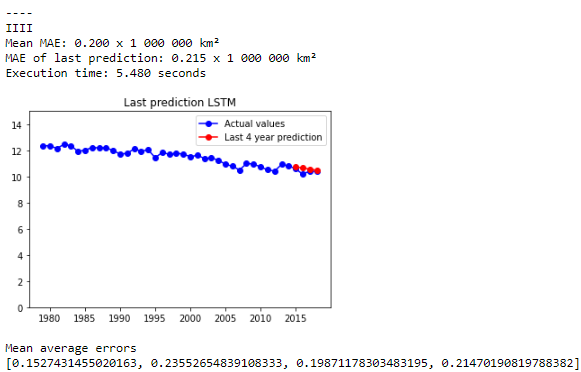
\includegraphics[width=1\linewidth]{uv_ns_LSTM}
\end{figure}

\clearpage
\subsection{Prophet}

Als laatste dient ook Prophet nog bekeken te worden voor het voorspellen van de tijdreeks. Hier zal eerst de data opnieuw geformateerd moeten worden aangezien prophet een bepaalde structuur hantereert.

\captionof{listing}{Code voor het formatteren van de data voor Prophet}
\begin{minted}[
frame=lines,
framesep=2mm,
fontsize=\footnotesize,
linenos,breaklines
]{python}
# formatting dataframe
ts_formated_prophet = ts_diff.reset_index().rename(columns = {'Year' : 'ds', 'ice_extent' : 'y'})
ts_formated_prophet['ds'] = pd.DataFrame(pd.to_datetime(ts_formated_prophet['ds'].astype(str), format='%Y'))
\end{minted}

Daarna kan de hyperparameter voor changepoint\textunderscore prior\textunderscore scale die zal staan voor de frequentie van het aanduiden changepoints (punten waar de data van een trend zal afwijken) bepaald worden met behulp van onderstaande code.

\captionof{listing}{Code voor het bepalen van de hyperparameters}
\begin{minted}[
frame=lines,
framesep=2mm,
fontsize=\footnotesize,
linenos,breaklines
]{python}

# Python
import itertools
import numpy as np
import pandas as pd

# define dataframe
df = ts_formated_prophet

param_grid = {  
'changepoint_prior_scale': [0.001, 0.01, 0.1, 1, 2, 5, 10, 15, 20, 25],
}

# Generate all combinations of parameters
all_params = [dict(zip(param_grid.keys(), v)) for v in itertools.product(*param_grid.values())]

# initialize variables
maes = []  
global_maes = []
best_MAE_prophet = np.inf

# Use cross validation to evaluate all parameters
for params in all_params:

    # loop trough all split time series that have a trainingsset with more than 20 values
    for train_index, test_index in tscv.split(ts_formated_prophet):    
        if train_index.size > 20:  
        
            # initialize cross validation train and test sets
            train  = ts_formated_prophet.iloc[train_index]
            y_test = ts_formated_prophet.iloc[test_index][['y']].values.flatten()
            X_test = ts_formated_prophet.iloc[test_index][['ds']]
            
            # Fit model with given params
            model = Prophet(**params, weekly_seasonality=False, daily_seasonality=False)
            model = model.fit(train)
            
            # make predictions
            forecast = model.predict(X_test)
            y_pred = forecast['yhat'].values
            
            # last actual prediction 
            last_prediction_prophet = y_pred
            
            # error calculation this part of the cross validation
            maes.append(mean_absolute_error(y_test, y_pred))
    
    # error calculation for this parameter combination
    MAE_prophet = np.mean(maes)
    last_MAE_prophet = maes[-1]
    global_maes.append(MAE_prophet)
    
    # logging
    print('changepoint_prior_scale: ' + str(params['changepoint_prior_scale']))
    
    # store parameters resulting in the lowest mean MAE
    if best_MAE_prophet > MAE_prophet:
    best_params = params
    best_MAE_prophet = MAE_prophet

# log optimal result          
print('changepoint_prior_scale: ' + str(best_params['changepoint_prior_scale']))
print(best_MAE_prophet)

\end{minted}

Hieruit zal blijken dat de optimale waarde voor de hyperparameter 2 is. Waneer dit ingevoegd wordt bij het uitvoeren van de onderstaande code wordt het resultaat dat zichtbaar is op figuur \ref{fig:uvnsprophet} verkregen.

\begin{figure}
    \centering
    \caption{Resultaat finale iteratie Prophet}
    \label{fig:uvnsprophet}
    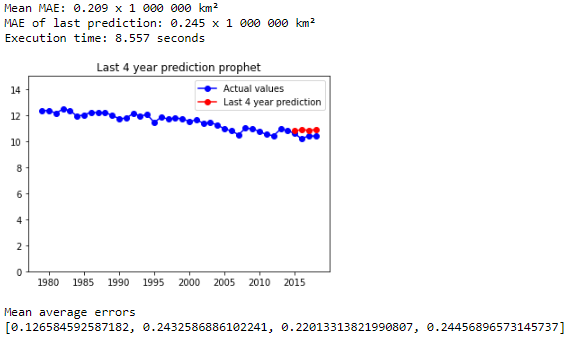
\includegraphics[width=1\linewidth]{uv_ns_prophet}
\end{figure}


\captionof{listing}{Finale iteratie Prophet}
\begin{minted}[
frame=lines,
framesep=2mm,
fontsize=\footnotesize,
linenos,breaklines
]{python}

%%time

# Disabled tf warning because of clutter
warnings.filterwarnings("ignore") # specify to ignore warning messages

start_time = timeit.default_timer()

# initialize variables
maes = []

for train_index, test_index in tscv.split(ts_formated_prophet):
    if train_index.size > 20:  
    
        # initialize cross validation train and test sets
        train  = ts_formated_prophet.iloc[train_index]
        y_test = ts_formated_prophet.iloc[test_index][['y']].values.flatten()
        X_test = ts_formated_prophet.iloc[test_index][['ds']]
        
        # build model
        model = Prophet(**best_params, weekly_seasonality=False, daily_seasonality=False)
        model.fit(train)
        
        # make predictions
        forecast = model.predict(X_test)
        y_pred = forecast['yhat'].values
        
        # error calc
        maes.append(mean_absolute_error(y_test, y_pred))
        
        # last actual prediction 
        last_prediction_prophet = y_pred


# store results
time_Prophet = timeit.default_timer() - start_time
MAE_Prophet = np.mean(maes)
last_MAE_Prophet = maes[-1]

# visualize results
print()
print('Mean MAE: %.3f x 1 000 000 km\u00b2' % MAE_Prophet)
print('MAE of last prediction: %.3f x 1 000 000 km\u00b2' % last_MAE_Prophet)
print('Execution time: %.3f seconds' % time_Prophet)
full_graph(last_prediction_prophet, "Last 4 year prediction prophet")
print('Mean average errors')
print(maes)

\end{minted}

\clearpage
\subsection{Evaluatie}

Wanneer deze resultaten gecombineerd worden wordt de tabel die zichtbaar is op figuur \ref{fig:uvnsresult} verkregen. Om dit resultaat grafisch te schetsen worden op figuur\ref{fig:uvnsresultgraph} de laatste voorspellingen voor elk modeltype weergegeven.

Hieruit kunnen dus geconcludeerd worden dat ARIMA het beste gemiddelde resultaat zal halen bij cross validation aangezien het hier een fout van 0.171 x 1 000 000 km\textsuperscript{2} behaalt. Ook de uitvoeringstijd is het laagst bij ARIMA namelijk 0.360 seconden. Dit is een beter dan LSTM met een fout van 0.200 x 1 000 000 km\textsuperscript{2} en een uitvoeringstijd van 5.480 seconden. De voorspelling van Prophet is nog een pak minder accuraat met een fout van 0.252 x 1 000 000 km\textsuperscript{2} en een uitvoeringstijd van 8.891 seconden.


\begin{figure}
    \centering
    \caption{Resultaat van de univariate non-seasonal analyse}
    \label{fig:uvnsresult}
    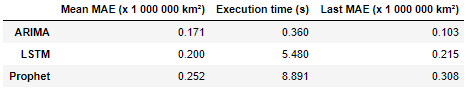
\includegraphics[width=0.7\linewidth]{uv_ns_result}
\end{figure}

\begin{figure}
    \centering
    \caption{Grafische weergave van de laatste voorspellingen van de univariate non-seasonal analyse}
    \label{fig:uvnsresultgraph}
    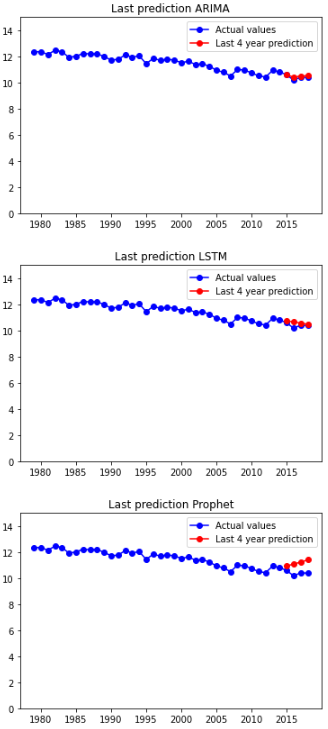
\includegraphics[width=0.7\linewidth]{uv_ns_result_graph}
\end{figure}



\captionof{listing}{Code voor het weergeven van de resultaten}
\begin{minted}[
frame=lines,
framesep=2mm,
fontsize=\footnotesize,
linenos,breaklines
]{python}
# formatting
results = [[MAE_ARIMA,time_ARIMA,last_MAE_ARIMA],[MAE_LSTM,time_LSTM,last_MAE_LSTM],[MAE_Prophet,time_Prophet,last_MAE_Prophet]]

# display results
pd.DataFrame(results, columns=['Mean MAE (x 1 000 000 km\u00b2)','Execution time (s)','Last MAE (x 1 000 000 km\u00b2)'],index=['ARIMA','LSTM','Prophet']).round(decimals=3)

\end{minted}

\captionof{listing}{Code voor het grafisch weergeven van de resultaten}
\begin{minted}[
frame=lines,
framesep=2mm,
fontsize=\footnotesize,
linenos,breaklines
]{python}
# visualize results of last prediction
full_graph(last_prediction_ARIMA, "Last prediction ARIMA")
full_graph(last_prediction_LSTM, "Last prediction LSTM")
full_graph(last_prediction_prophet, "Last prediction Prophet")
\end{minted}

\clearpage

\section{Univariate seizoensgebonden}

In deze sectie zal onderzocht worden welk type model de beste voorspellingen zal treffen voor data met 1 variabele waar er een duidelijk seizoensverband zichtbaar is. Ook hier zal crossvalidation gebruikt worden maar het aantal minimum waarden in de trainingsset zal hier niet 20 zijn maar 300.

\subsection{Algemene methodes}

Vooraleer de dataset effectief gebruikt zal worden dienen er eerst nog enkele functies gedeclareerd te worden.

Zo herkennen kunnen de test\textunderscore stationarity, full\textunderscore graph en  revert\textunderscore diff methodes van de voorgaande sectie herkend worden. Naast deze methodes wordt hier ook nog de revert\textunderscore seasonal\textunderscore diff\textunderscore recursion methode gedefinieerd. Deze wordt benut bij de seizoensgebonden variant van de revert\textunderscore diff methode namelijk revert\textunderscore seasonal\textunderscore diff. Ook deze methode zal dienen om een gedifferentieerde data terug om te zetten naar data die vergeleken kan worden met de effectieve waarden.


\captionof{listing}{Algemene methodes}
\begin{minted}[
frame=lines,
framesep=2mm,
fontsize=\footnotesize,
linenos,breaklines
]{python}
def test_stationarity(timeseries):

    #Determing rolling statistics
    rolmean = timeseries.rolling(36).mean()
    rolstd = timeseries.rolling(24).std()
    
    #Plot rolling statistics:
    orig = plt.plot(timeseries, color='blue',label='Original')
    mean = plt.plot(rolmean, color='red', label='Rolling Mean')
    std = plt.plot(rolstd, color='black', label = 'Rolling Std')
    plt.legend(loc='best')
    plt.title('Rolling Mean & Standard Deviation')
    plt.show(block=False)

def full_graph(predicted, og_dataset, title):
    zerosArray = np.zeros(og_dataset.values.size-len(predicted.flatten()))
    cleanPrediction = pd.Series(np.concatenate((zerosArray,predicted))).replace(0,np.NaN)
    
    # plot
    plt.title(title)
    plt.plot(og_dataset.index, og_dataset.values,marker='o', color='blue',label='Actual values')
    plt.plot(og_dataset.index, cleanPrediction,marker='o', color='red',label='Last 2 year prediction')
    plt.ylim([0,20])
    plt.legend()
    
    plt.show()

def revert_diff(predicted_diff, og_data):
    last_value = og_data.iloc[-predicted_diff.size-1][0]
    predicted_actual = np.array([])
    for value_diff in predicted_diff:
    actual_value = last_value + value_diff
    predicted_actual = np.append(predicted_actual, actual_value)
    last_value = actual_value
    return predicted_actual

def revert_seasonal_diff_recursion(last_seasons_value, diff_value):
    return last_seasons_value + diff_value

def revert_diff_seasonal(predicted_diff, og_data):
    prediction_size = predicted_diff.size

    history = ts[:-prediction_size].values.flatten()
    for value_diff in predicted_diff[-prediction_size:]:
        new_value = revert_seasonal_diff_recursion(history[-12], value_diff)
        history = np.append(history,new_value)
    return history[-prediction_size:]
\end{minted}

\subsection{Stationariteit}

Ook wanneer we hier de stationariteit van de data gaan testen krijgen we een licht dalende trend. Deze trend die zichtbaar is op figuur \ref{fig:uvsstationarity}. Deze loopt gelijk met de trend van de niet seizoensgebonden data aangezien die data het jaarlijks gemiddelde is en dit maandelijkse waarden zijn.

\begin{figure}
    \centering
    \caption{Stationariteit van de originele univariate seizoensgebonden data}
    \label{fig:uvsstationarity}
    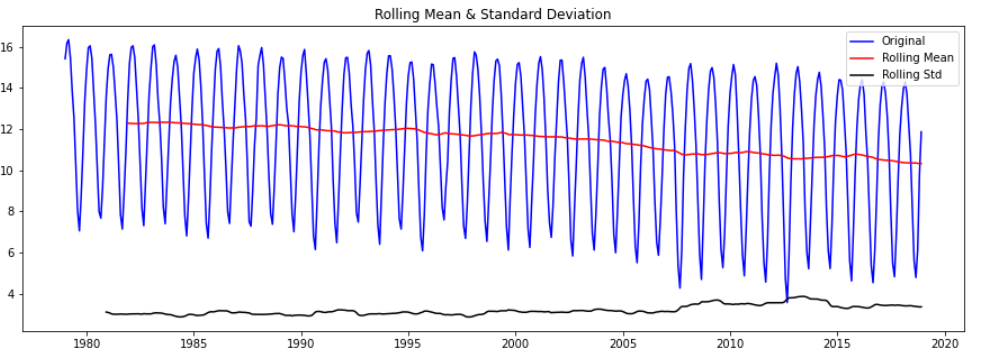
\includegraphics[width=1\linewidth]{uvsstationarity}
\end{figure}

Aangezien hier met seizoensgebonden data gewerkt wordt is het hier naast random walk differentiatie een optie om seizoensdifferentiatie te gebruiken. Dit zal dan ook getest worden. 

\captionof{listing}{Code voor seizoensdifferentiatie}
\begin{minted}[
frame=lines,
framesep=2mm,
fontsize=\footnotesize,
linenos,breaklines
]{python}
ts_diff_seasonal = ts - ts.shift(12)
ts_diff_seasonal = ts_diff_seasonal.dropna()
test_stationarity(ts_diff_seasonal)
\end{minted}

Wanneer seizoensdifferentiatie toegepast wordt zal de stationariteit voorgesteld kunnen worden zoals zichtbaar op figuur\ref{fig:uvsstationarityseasonal}. Dit is wel stationair maar fluctureert wel behoorlijk naar het einde toe.

\begin{figure}
    \centering
    \caption{Stationariteit van de data na seizoensdifferentiatie}
    \label{fig:uvsstationarityseasonal}
    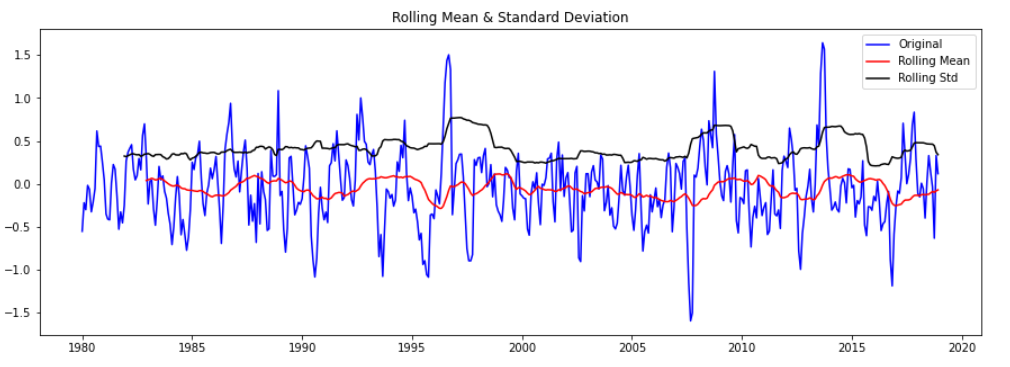
\includegraphics[width=1\linewidth]{uvsstationarityseasonal}
\end{figure}

Daarnaast kan ook nog gewone random walk differentiatie toegepast worden op de data. De stationariteit van deze gedifferentieerde data wordt afgebeeld op figuur\ref{fig:uvsstationarityrw}. Hier wordt vastgesteld dat het gemiddelde een horizontale lijn is. Dit houdt in dat de data zeer stationair is.

\begin{figure}
    \centering
    \caption{Stationariteit van de data na random walk differentiatie}
    \label{fig:uvsstationarityrw}
    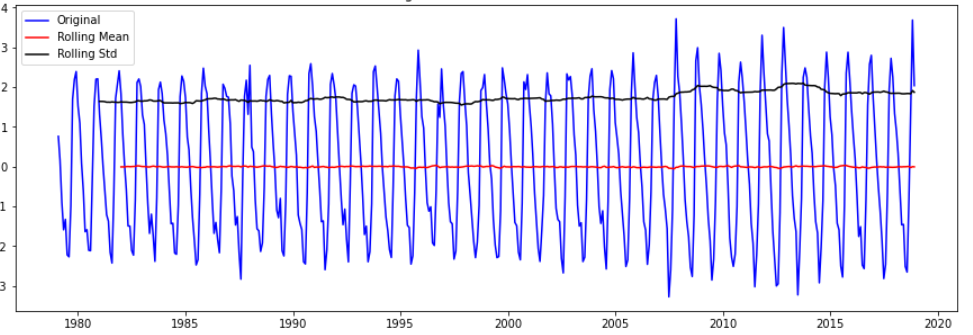
\includegraphics[width=1\linewidth]{uvsstationarityrw}
\end{figure}


\captionof{listing}{code voor differentiatie}
\begin{minted}[
frame=lines,
framesep=2mm,
fontsize=\footnotesize,
linenos,breaklines
]{python}
ts_diff = ts - ts.shift(1)
ts_diff = ts_diff.dropna()
test_stationarity(ts_diff)
\end{minted}

Er dient ook nog vermeld te worden dat door 2 verschillende types differentiaties te testen, het aantal gebruikte testsets bij crossvalidation wel verschillen. Zo zullen er bij seizoensdifferentiatie minder waarden beschikbaar zullen zijn. Concreet leidt dit ertoe dat er bij random walk differentiatie 7 trainingssets zijn die meer dan 300 waarden bevatten terwijl er bij seizoensdifferentiatie 6 trainingssets zullen zijn die meer dan 300 waarden bevatten.

\subsection{ARIMA}

Ook hier zal een ARIMA model opgesteld worden zowel voor de random walk gedifferentieerde data als de seizoensgedifferentieerde data.
\subsubsection{Random walk differentiatie}

Ook hier zal aan hyperparameterbepaling gedaan worden. Aangezien zo goed als alles identiek is als bij univariate non-seasonal differentiatie zal de code hiervan niet meer weergegeven worden alle code is echter terug te vinden in de bijlage.

Uit die hyperparameterbepaling zal blijken dat de combinatie (3,0,4) de beste prestatie zal leveren wanneer het bereik van de parameters $p$ en $q$ 5 zal zijn. 

Wanneer deze hyperparameters ingevoerd worden wordt het resultaat dat afgebeeld staat op figuur \ref{fig:uvsarimadiff} verkregen.

\begin{figure}
    \centering
    \caption{Resultaat van ARIMA bij random walk differentiatie}
    \label{fig:uvsarimadiff}
    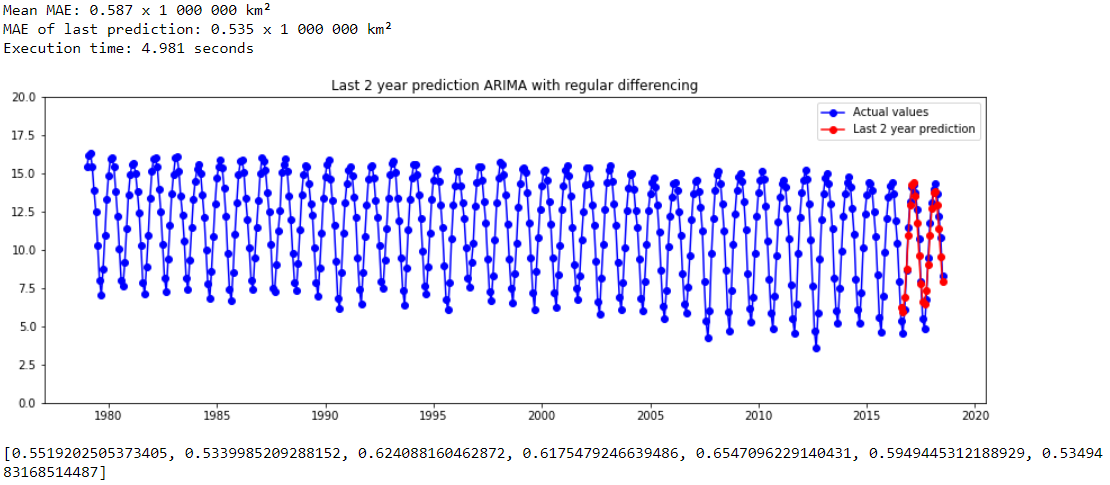
\includegraphics[width=1\linewidth]{uv_s_arima_diff}
\end{figure}


\subsubsection{Seizoensdifferentiatie}

Ook hier zullen eerst de hyperparameters bepaald worden. Met (3,0,3) als optimale waarden bij een range van 0 tot 5 voor de waarden $p$ of $q$. Wanneer deze waarden uitgebreider getest worden resulteert dit in de uitvoer die waar te nemen valt op figuur\ref{fig:uvsarimasdiff}.


\begin{figure}
    \centering
    \caption{Resultaat van ARIMA bij seizoensdifferentiatie}
    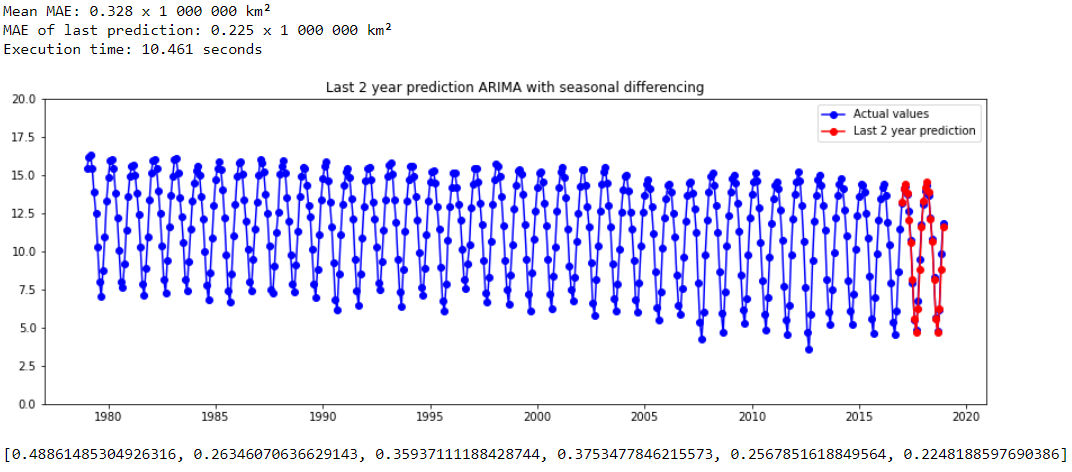
\includegraphics[width=1\linewidth]{uv_s_arima_sdiff}
    \label{fig:uvsarimasdiff}
\end{figure}

\subsection{SARIMA}

Naast ARIMA zelf is er ook een variant op het ARIMA model die specifiek voor data met een seizoenseffect is ontworpen genaamd SARIMA. Deze variant zal in dit deel onder de loep genomen worden.

\subsubsection{Random walk differentiatie} 

De hyperparameterbepaling zal er hier wel anders uitzien, zo dienen voor het seizoenseffect $PDQ$ waarden bepaald te worden naast de $pdq$ waarden voor de data zelf en de $m$ waarde die het aantal tijdstappen zal weergeven van de data die binnen 1 sequentie van het seizoenseffect vallen.

De beste parametercombinatie van de parameters $p, d, q, P, D, Q$ met een bereik van 3 zal (1,0,2,0,1,2) zijn. Het uitgebreid resultaat van deze combinatie wordt weergegeven op figuur\ref{fig:uvssarimaxdiff}.

\begin{figure}
    \centering
    \caption{Resultaat SARIMAX bij random walk differentiatie}
    \label{fig:uvssarimaxdiff}
    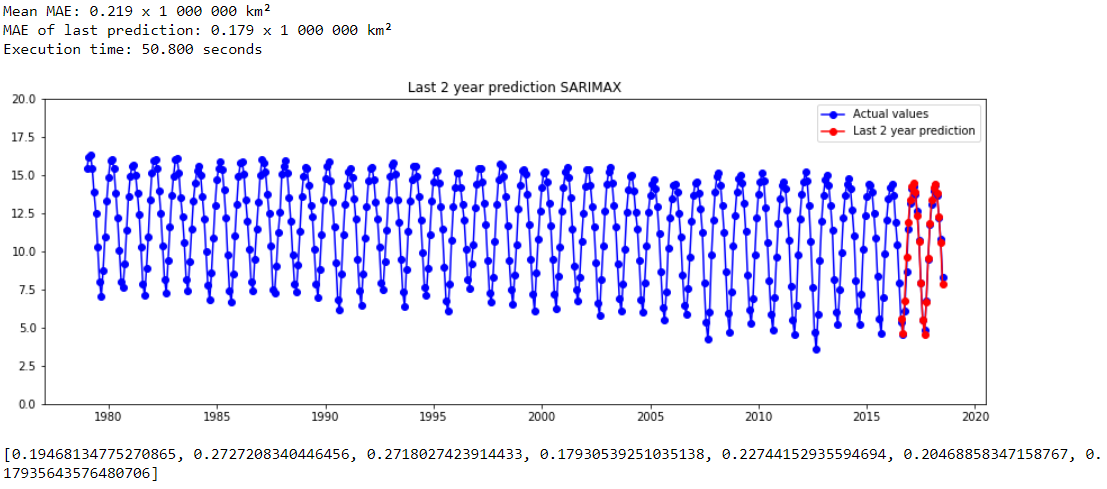
\includegraphics[width=1\linewidth]{uv_s_sarimax_diff}
\end{figure}


\subsubsection{Seizoensdifferentiatie}

Deze testopstelling is identiek aan de vorige uitgezonderd van de invoerdata die hier seizoensgedifferentieerd zal zijn. Ook hier zullen de optimale parameters (1,0,2,0,1,2) zijn. Dit de uitvoer geven die afgebeeld staat op figuur \ref{fig:uvssarimaxsdiff}.

\begin{figure}
    \centering
    \caption{Resultaat SARIMAX bij seizoensdifferentiatie}
    \label{fig:uvssarimaxsdiff}
    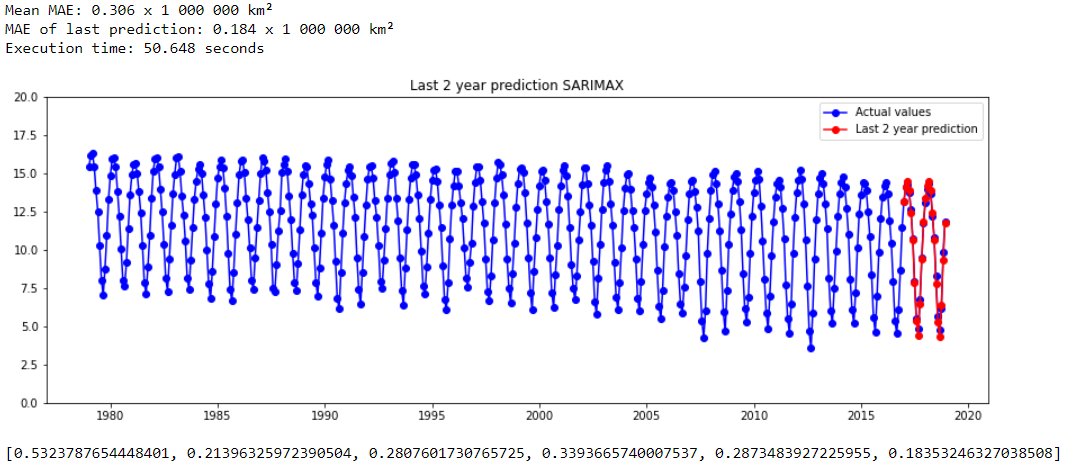
\includegraphics[width=1\linewidth]{uv_s_sarimax_s_diff}
\end{figure}

\subsection{LSTM}
\subsubsection{Random walk differentiatie}

%Ook de opbouw van het LSTM bij seizoensgebonden univariate data verloopt net als die bij niet seizoensgebonden univariate data. Hier bleek er echter wel een verschil in resultaat bij de verschillende hyperparameters en de optimale configuratie met de testwaarden bleek een model te zijn met 1 neuron, waar de dropout rate 0.99 was en een batchgrootte die 8 bedroeg. Het eindresultaat van deze configuratie staat afgebeeld op figuur \ref{fig:uvslstmdiff}.

\subsubsection{Seizoensdifferentiatie}

De opstelling zal identiek zijn als de bovenstaande hier zullen de optimale parameters bestaan uit 1 neuron een dropout rate van 0.99 en een batchgrootte van 8 met het eindresultaat dat zich op figuur \ref{fig:uvslstmsdiff} bevindt.

\begin{figure}
    \centering
    \caption{Resultaat LSTM bij seizoensdifferentiatie}
    \label{fig:uvslstmsdiff}
    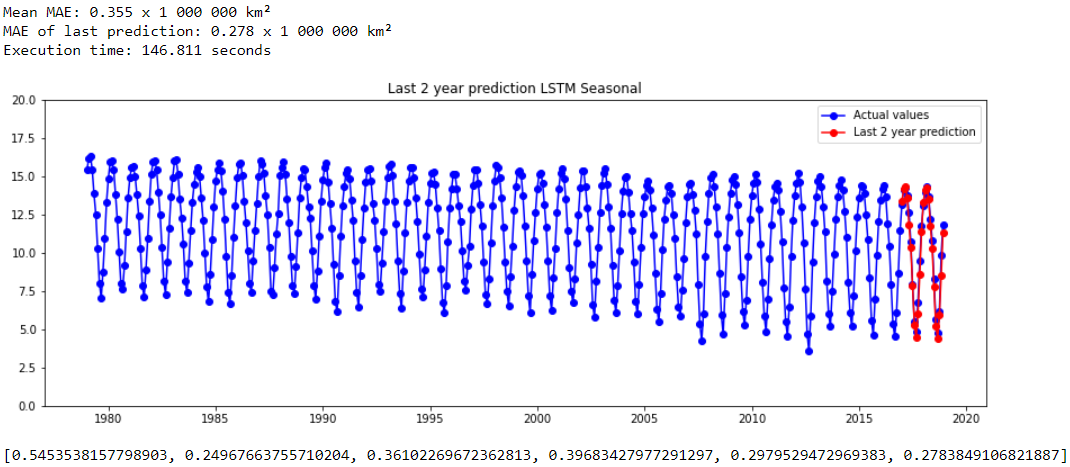
\includegraphics[width=1\linewidth]{uv_s_lstm_s_diff}
\end{figure}

\clearpage
\subsection{Prophet}

Ook hier verloopt alles bijna analoog met de niet seizoensgebonden variatie behalve dat er hier wel 2 hyperparameters getest worden, aangezien er hier wel een seizoenseffect aanwezig is kan de de variabele seasonality\textunderscore prior\textunderscore scale ook onderzocht worden. Het laatste resultaat van de reeks wordt weergegeven op Figuur \ref{fig:uvsprophet}.

\begin{figure}
    \centering
    \caption{Resultaten de voorspellingen voor univariate seizoensgebonden data met Prophet}
    \label{fig:uvsprophet}
    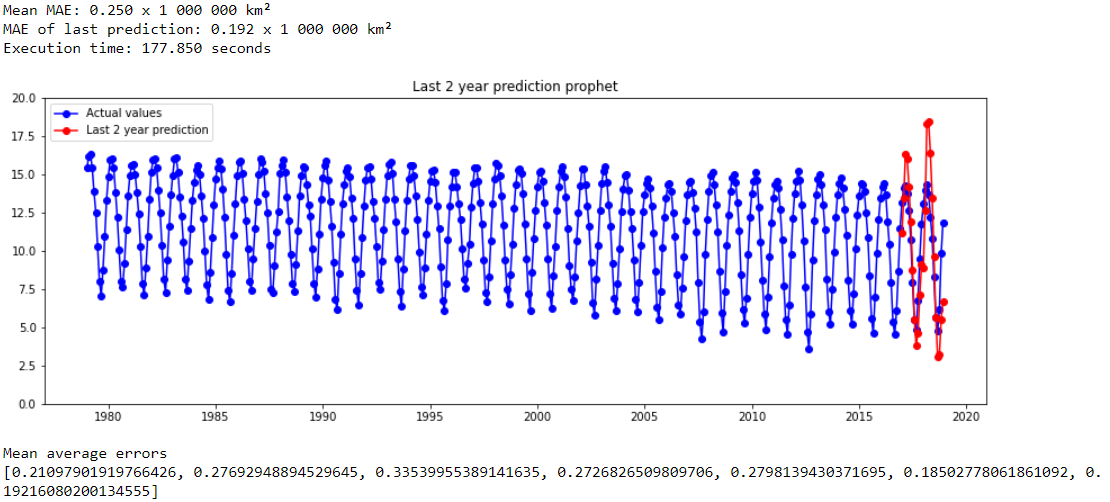
\includegraphics[width=1\linewidth]{uv_s_prophet}
\end{figure}

\clearpage
\subsection{Evaluatie}

Wanneer we de resultaten afgebeeld op Figuur \ref{fig:uv_s_results} beschouwen kunnen we concluderen dat SARIMA met random walk differentiatie de beste voorspellingen zal treffen wanneer we de gemiddelde MAE beschouwen namelijk 0.219 (x 1 000 000 km\textsuperscript{2}). Ook de laatste voorspelling is de meest accurate van alle modellen. Ook de uitvoeringstijd van SARIMA met random walk differencing is relatief laag enkel de ARIMA modellen zijn sneller maar die zijn een stuk minder accuraat.
Het SARIMA-model dat werkt met seizoensgedifferentieerde data presteert een stuk slechter met een gemiddelde MAE van 0.360 (x 1 000 000 km\textsuperscript{2})
\\

Daarnaast presteert het Prophet-model ook goed met een gemiddelde MAE van 0.250 (x 1 000 000 km\textsuperscript{2}) al heeft het wel de op \'{e}\'{e}n na langste uitvoeringstijd. Het ARIMA-model met seizoensdifferentiatie heeft een gemiddelde MAE van 0.328 (x 1 000 000 km\textsuperscript{2}) maar heeft wel de kortste uitvoeringstijd.
De LSTM modellen scoren beide vrij slecht met hoge uitvoeringstijden dus deze vallen niet aan te raden met deze implementatie om seizoensgebonden tijdreeksen te voorspellen.
\\

Bij seizoensgebonden data presteren de LSTM- en ARIMA-modellen beter wanneer er aan seizoensdifferentiatie gedaan wordt, maar de implementatie met random walk differentiatie behaalt de beste score bij SARIMAX dus er kan niet gesteld worden dat de ene soort differentiatie altijd effectiever zal zijn dan de andere. De laatste voorspellingen van alle modeltypes worden weergegeven op Figuren \ref{fig:uvsgraph1} en \ref{fig:uvsgraph2}.


\begin{figure}
    \centering
    \caption{Resultaten van de univariate seizoensgebonden voorspellingen}
    \label{fig:uv_s_results}
    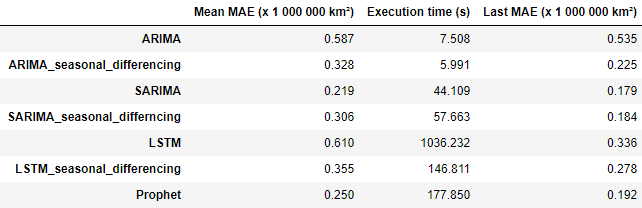
\includegraphics[width=0.9\linewidth]{uv_s_results}
\end{figure}

\begin{figure}
    \centering
    \caption{Grafische weergaven van de laatste voorspellingen van univariate seizoensgebonden data (deel 1)}
    \label{fig:uvsgraph1}
    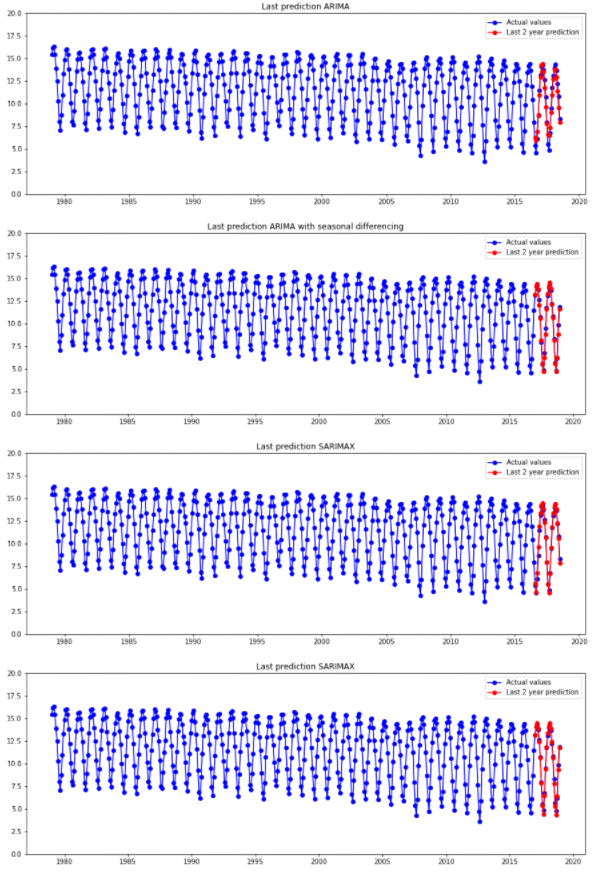
\includegraphics[width=1\linewidth]{uv_s_graph1}
\end{figure}

\begin{figure}
    \centering
    \caption{Grafische weergaven van de laatste voorspellingen van univariate seizoensgebonden data (deel 2)}
    \label{fig:uvsgraph2}
    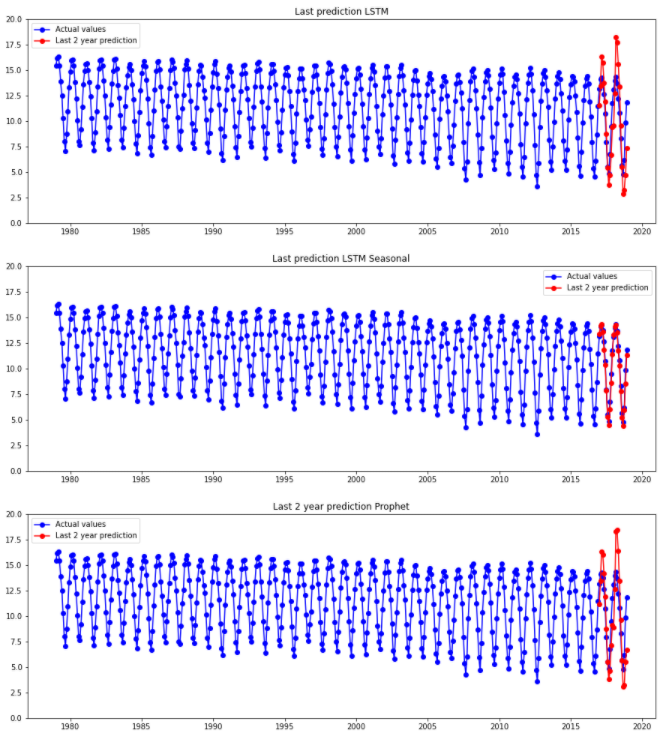
\includegraphics[width=1\linewidth]{uv_s_graph2}
\end{figure}


\section{Multivariate niet-seizoensgebonden}
In dit onderdeel van deze bachelorproef zal onderzocht worden welk van de 3 modellen de beste voorspelling maken voor meervoudige tijdreeksen. Dit houdt in dat het model een tijdreeks krijgt die meerdere features bevat per tijdstap en deze features in verband brengt om tot accuratere voorspellingen te komen. De testset zal dan ook altijd enkel blijven bestaan uit de tijdsstappen die voorspeld moeten worden.

De data die gebruikt zal worden voor deze sectie wordt grafisch weergegeven op Figuur \ref{fig:mvnsdata}. Ook hier zal er gebruik gemaakt worden van cross validation.

Aangezien Prophet geen multivariate tijdreeksen als invoer ondersteunt zal dit niet ge\"{e}valueerd kunnen worden.

\begin{figure}
    \centering
    \caption{Grafische weergave multivariate tijdreeks zonder seizoenseffect}
    \label{fig:mvnsdata}
    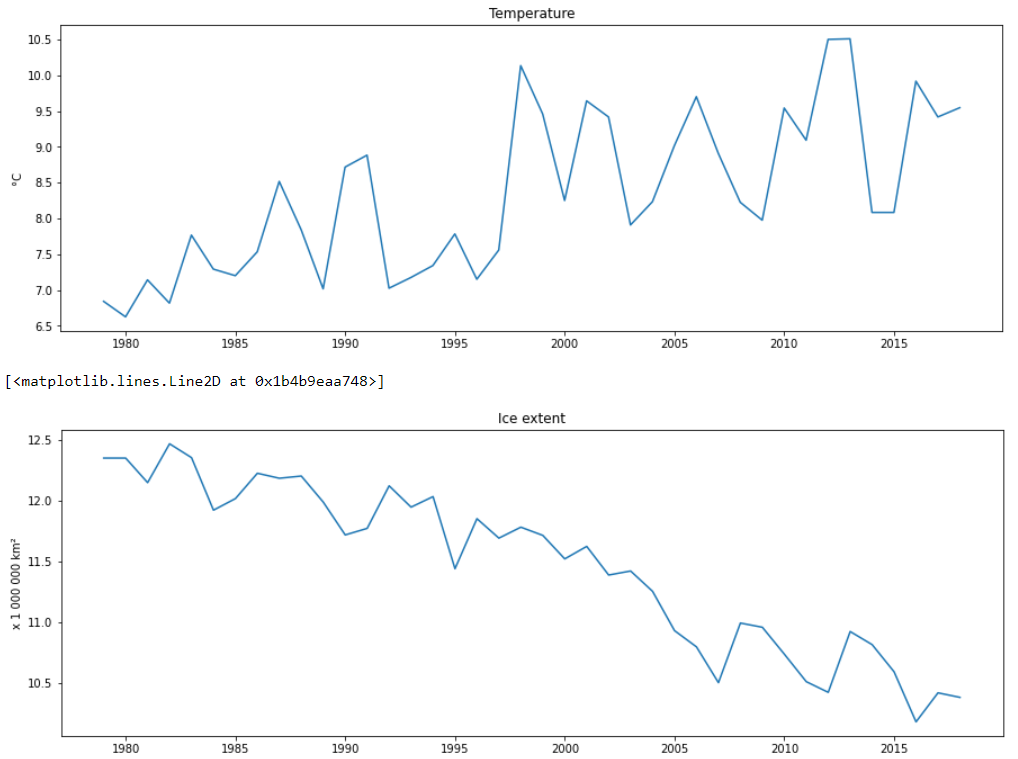
\includegraphics[width=1\linewidth]{mv_ns_data}
\end{figure}

\subsection{Stationariteit}

Ook hier zal de ijsdikte een dalende trend vertonen zoals weergegeven werd bij de univariate analyse en hier zal niks aan veranderen aangezien dit dezelfde data is. Ook deze data zal random walk gedifferentieerd worden maar dit keer niet enkel de ijsdikte maar ook de temperatuur. De resultaten van die differentiatie zijn zichtbaar op figuur \ref{fig:mvnsdatadiff}. Daaruit kan afgeleid worden dat de data nu stationair is.

\begin{figure}
    \centering
    \caption{Grafische weergave gedifferentieerde multivariate tijdreeks zonder seizoenseffect}
    \label{fig:mvnsdatadiff}
    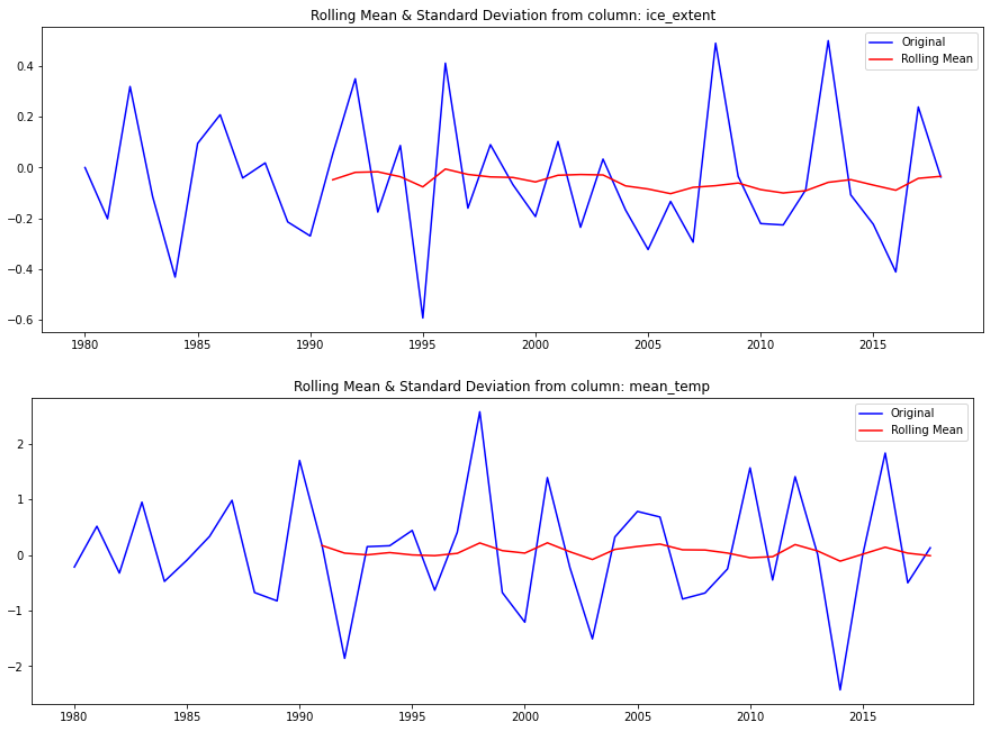
\includegraphics[width=1\linewidth]{mv_ns_data_diff}
\end{figure}

\subsection{VARMAX}
Aangezien een ARIMA model slechts in staat is om tijdreeksen met 1 variabele te voorspellen moet er een variant gebruikt worden die wel in staat is om multivariate tijdreeksen te interpreteren genaamd VARMAX. 

Ook hier wordt de gebruikelijke methode toegepast om de hyperparameters te bepalen en daar verandert niet veel aan. Behalve dat enkel de $p$ en $q$ variabelen verwacht worden, de $d$ variabele is hier niet nodig. 

Bij een range van 0 tot 5 zijn ook hier de optimale waarden voor deze parameters (3,3). Wanneer we deze waarden invoeren in de uitgebreidere versie van de evaluatiemethode wordt het resultaat bekomen dat weergegeven wordt op Figuur \ref{fig:mvnsvarmax}.

\begin{figure}
    \centering
    \caption{Resultaat multivariate voorspelling VARMAX}
    \label{fig:mvnsvarmax}
    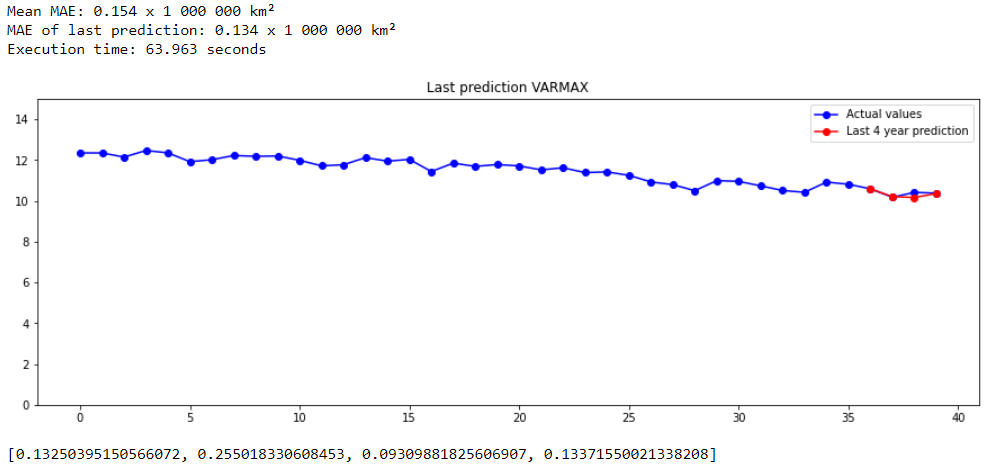
\includegraphics[width=1\linewidth]{mv_ns_varmax}
\end{figure}


\subsection{LSTM}

Waneer er multivariate voorspellingen gemaakt moeten worden met LSTM ziet de structuur van het neuraal netwerk er anders uit dan bij een univariate voorspelling. Zo zal er deze keer een grote functie gebruikt worden om het model op te stellen en de voorspelling te maken. Deze functie staat uitgeschreven bij listing \ref{code:pred_lstm}.

De hyperparameters die hier bepaald zullen worden zijn het aantal neuronen en het aantal epochs om tot het beste resultaat te komen. Een enkel neuron blijkt alweer optimaal te zijn en met 200 epochs verkrijgt men het beste resultaat. De uitgebreide uitvoer van dit resultaat wordt weergegeven op Figuur \ref{fig:mvnslstm}.

\captionof{listing}{Voorspellingsfunctie LSTM}
\label{code:pred_lstm}
\begin{minted}[
frame=lines,
framesep=2mm,
fontsize=\footnotesize,
linenos,breaklines
]{python}
def predict_LSTM(train, test, n_neurons, n_epochs):
    test['sum'] = test['mean_temp'] + test['ice_extent']
    
    
    # define input sequence
    in_seq1 = train.values[:,0]
    in_seq2 = train.values[:,1]
    out_seq = array([in_seq1[i]+in_seq2[i] for i in range(len(in_seq1))])
    
    # convert to [rows, columns] structure
    in_seq1 = in_seq1.reshape((len(in_seq1), 1))
    in_seq2 = in_seq2.reshape((len(in_seq2), 1))
    out_seq = out_seq.reshape((len(out_seq), 1))
    
    # horizontally stack columns
    dataset = hstack((in_seq1, in_seq2, out_seq))
    
    # choose a number of time steps
    n_steps_in, n_steps_out = 4, 4
    
    # covert into input/output
    X, y = split_sequences(dataset, n_steps_in, n_steps_out)
    
    # the dataset knows the number of features, e.g. 2
    n_features = X.shape[2]
    
    # define model
    model = Sequential()
    model.add(LSTM(n_neurons, activation='relu', input_shape=(n_steps_in, n_features)))
    model.add(RepeatVector(n_steps_out))
    model.add(LSTM(n_neurons, activation='relu', return_sequences=True))
    model.add(TimeDistributed(Dense(n_features)))
    model.compile(optimizer='adam', loss='mae')
    
    # fit model
    model.fit(X, y, epochs=n_epochs, verbose=0)
    
    # demonstrate prediction
    x_input = test.values
    x_input = x_input.reshape((1, n_steps_in, n_features))
    yhat = model.predict(x_input, verbose=0)
    return yhat
\end{minted}

\begin{figure}
    \centering
    \caption{Resultaat multivariate voorspelling LSTM}
    \label{fig:mvnslstm}
    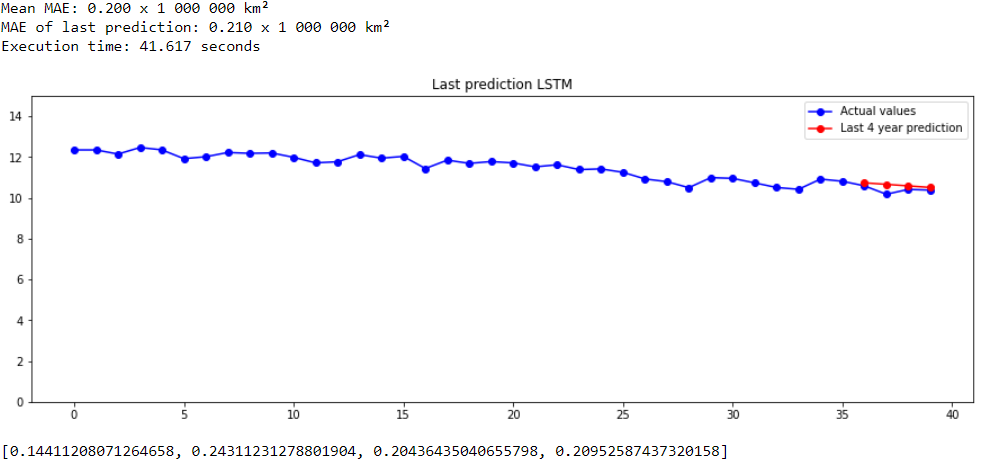
\includegraphics[width=1\linewidth]{mv_ns_LSTM}
\end{figure}
\clearpage

\subsection{Evaluation}

Wanneer we de resultaten van de multivariate niet-seizoensgebonden voorspellingen weergegeven op Figuur \ref{fig:mvnsresult} vergelijken kunnen we stellen dat VARMAX het best presteert volgens cross validation maar wel een hogere uitvoeringstijd heeft. Daarnaast zal de laatste voorspelling van het ijsoppervlak door het VARMAX model ook accurater zijn dan dat van het LSTM model. Deze laatste voorspelling wordt grafisch weergegeven op Figuur \ref{fig:mvnsresultgraph}.

\begin{figure}
    \centering
    \caption{Resultaten multivariate voorspelling}
    \label{fig:mvnsresult}
    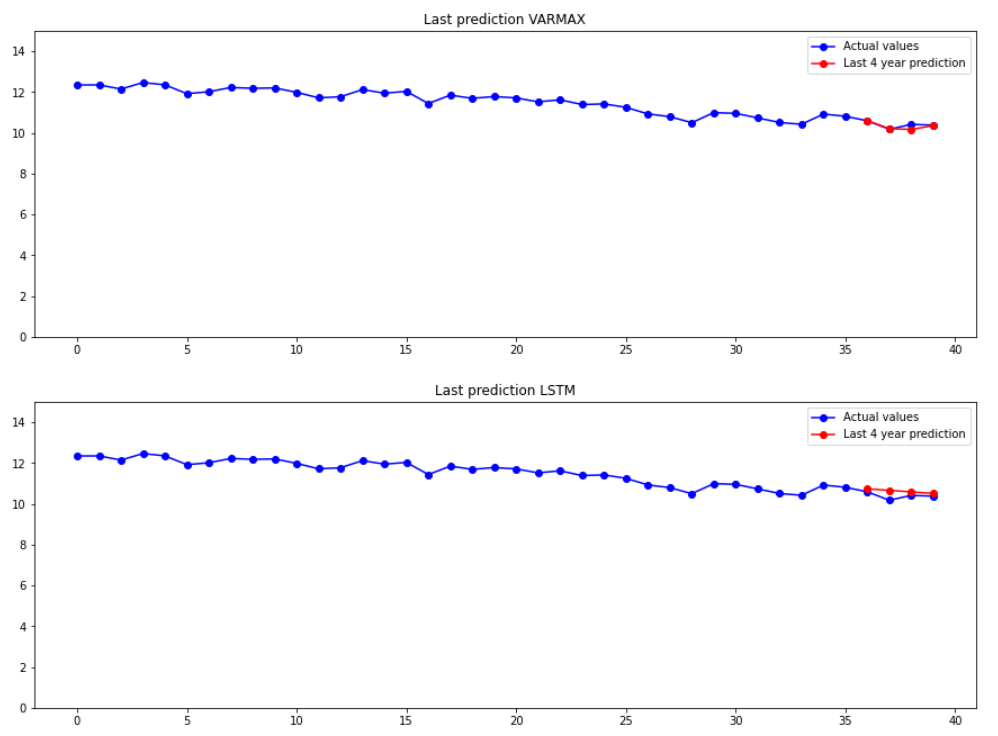
\includegraphics[width=1\linewidth]{mv_ns_result}
\end{figure}

\begin{figure}
    \centering
    \caption{Grafische weergaven van de laatste voorspellingen van de VARMAX en LSTM modellen}
    \label{fig:mvnsresultgraph}
    \includegraphics[width=1\linewidth]{mv_ns_result_graph}
\end{figure}



\section{Multivariate seizoensgebonden}

De laatste combinatie die getest zal worden is de dataset waar een seizoensverband en een extra variabele aanwezig is. Deze extra variabele zal andermaal de temperatuur zijn in een dataset die de maandelijkse temperatuur en ijsdikte zal bevatten. Hier zullen ook, net als bij de niet seizoensgebonden data, enkel VARMAX en LSTM getest worden. Hier zal ook weer cross validation gebruikt worden. Er zal ook weer random walk en seasonal differentiatie gebuikt worden.

\subsection{VARMAX}
\subsubsection{Random walk differentiatie}

Waneer we de hyperparameters bepalen bij dit VARMAX model blijken de parameters (4,1) de optimale waarden te zijn bij een range van 0 tot 5. Wanneer we deze invoeren om een uitgebreider resultaat te krijgen bekomen we de uitvoer die te beschouwen valt op Figuur \ref{fig:mvsvarmaxdiff}.

\begin{figure}
    \centering
    \caption{Resultaat VARMAX bij random walk differentiatie}
    \label{fig:mvsvarmaxdiff}
    \includegraphics[width=1\linewidth]{mv_s_varmax_diff}
\end{figure}


\subsubsection{Seizoensdifferentiatie}
De optimale hyperparameters bij het VARMAX model dat opgebouwd wordt op basis van seizoensgedifferentieerde data zijn (0,1) wanneer de range van 0 tot 5 loopt. Het resultaat van dit model wordt afgebeeld op Figuur \ref{fig:mvsvarmaxsdiff}.


\begin{figure}
    \centering
    \caption{Resultaat VARMAX bij seizoensdifferentiatie}
    \label{fig:mvsvarmaxsdiff}
    \includegraphics[width=1\linewidth]{mv_s_varmax_s_diff}
\end{figure}


\subsection{LSTM}
\subsubsection{Random walk differentiatie}
De optimale parameters bij Random walk differentiatie en bleken 30 neuronen te zijn en 300 epochs. Een hoger aantal neuronen en epochs zouden leiden tot een beter resultaat aangezien de MAE verlaagde naargelang deze parameters verhoogden maar er moest een grens getrokken worden om de uitvoeringstijd beperkt te houden. Wanneer we het model met de aangegeven parameters analyseren zullen we het resultaat bekomen dat op Figuur \ref{fig:mvslstmdiff}.

\begin{figure}
    \centering
    \caption{Resultaat LSTM bij random walk differentiatie}
    \label{fig:mvslstmdiff}
    \includegraphics[width=1\linewidth]{mv_s_lstm_diff}
\end{figure}


\subsubsection{Seizoensdifferentiatie}
De parameters die voor het beste resultaat zorgen bij het LSTM-model en seizoensgedifferentieerde data zijn 1 voor het aantal neuronen en 200 voor het aantal epochs en in tegenstelling tot de random walk differentiatie blijkt het verhogen van deze parameters niet te zorgen voor betere resultaten. Het resultaat van dit model wordt afgebeeld op Figuur \ref{fig:mvslstmsdiff}.


\begin{figure}
    \centering
    \caption{Resultaat LSTM seizoensdifferentiatie}
    \label{fig:mvslstmsdiff}
    \includegraphics[width=1\linewidth]{mv_s_lstm_s_diff}
\end{figure}

\clearpage

\subsection{Evaluation}
Wanneer we de resultaten op figuur \ref{fig:mvsresults} beschouwen kunnen we duidelijk aflezen dat LSTM met random walk differencing de laagste gemiddelde fout zal hebben en dus het best zal scoren wanneer we ons baseren op cross validation. Het scoort een stuk beter dan de andere modellen die allemaal een zeer gelijkaardige MAE hebben. Dit model zal echter wel de hoogste uitvoeringstijd hebben. \\

Het VARMAX model met seizoensdifferentiatie zal de beste score behalen wanneer we naar de laatste voorspelling kijken en zal ook de laagste uitvoeringstijd hebben dus dit zou op vlak van uitvoeringssnelheid een goed alternatief zijn. De grafische weergaven van de laatste voorspellingen zijn zichtbaar op Figuur \ref{fig:mvsresultsgraphs}. De waarden tussen de modellen die random walk differentiatie gebruiken zullen ietwat verschillen van degene die gebruik maken van seizoensdifferentiatie aangezien de data met 5 tijdstappen getransformeerd moest worden om tot evenwaardige testsetgroottes te komen. Dit was noodzakelijk om alle modellen met elkaar te vergelijken.


\begin{figure}
    \centering
    \caption{Resultaten multivariate seizoensgebonden voorspellingsmodellen}
    \label{fig:mvsresults}
    \includegraphics[width=0.8\linewidth]{mv_s_results}
\end{figure}


\begin{figure}
    \centering
    \caption{Grafische weergaven van de laatste voorspellingen van multivariate seizoensgebonden voorspellingsmodellen}
    \label{fig:mvsresultsgraphs}
    \includegraphics[width=1\linewidth]{mv_s_results_graphs}
\end{figure}




% Voeg hier je eigen hoofdstukken toe die de ``corpus'' van je bachelorproef
% vormen. De structuur en titels hangen af van je eigen onderzoek. Je kan bv.
% elke fase in je onderzoek in een apart hoofdstuk bespreken.

%\input{...}
%\input{...}
%...

%%=============================================================================
%% Conclusie
%%=============================================================================

\chapter{Conclusie}
\label{ch:conclusie}

% TODO: Trek een duidelijke conclusie, in de vorm van een antwoord op de
% onderzoeksvra(a)g(en). Wat was jouw bijdrage aan het onderzoeksdomein en
% hoe biedt dit meerwaarde aan het vakgebied/doelgroep? 
% Reflecteer kritisch over het resultaat. In Engelse teksten wordt deze sectie
% ``Discussion'' genoemd. Had je deze uitkomst verwacht? Zijn er zaken die nog
% niet duidelijk zijn?
% Heeft het onderzoek geleid tot nieuwe vragen die uitnodigen tot verder 
%onderzoek?

Uit dit onderzoek blijkt dat een voorspelling op basis van polynomiale regressie of LSTM het einde van de coronacrisis moeilijk kan definiëren. Het einde van de crisis houdt in dat het aantal nieuwe geregistreerde coronagevallen in België gedurende 2 weken onder 55 zou blijven. Een betrouwbare voorspelling is slechts voor 1 maximum, 2 weken mogelijk met gebruik van LSTM wat een te kort tijdsinterval is om dit te bepalen. Dit wordt hoogstwaarschijnlijk veroorzaakt door het gebrek aan data om het LSTM model te trainen. 
het model werd getraind met Italiaanse data, aangezien Italië    het meest nabije land dat al het langst voorbij het minimum van 10 gevallen per miljoen inwoners is. Dit komt neer op een voorloopperiode van een 7 tal dagen in vergelijking met België. Hierdoor kan het model slechts echt betrouwbare voorspellingen van iets meer dan 7 dagen maken.

Mogelijke onderwerpen voor verder onderzoek zouden dezelfde vraag kunnen beantwoorden maar met gebruik van andere data en middelen. Zo zou een multivatiate timeseries ook voorspeld kunnen worden met LSTM, een andere zeer interessante parameter zou de besmettingsgraad zijn bij deze vraag. Een andere type model om autoregressieve voorspellingen te maken zou het TP-SMN-AT model zijn. Een methode en ook de methode die het nauwst aansluit bij dit onderzoek zou het fitten van een hyperbolisch-achtige functie op de staart, de metingen en eventueel voorspellingen na de piek. Ook hierbij kunnen de curves van andere landen in beschouwing genomen. Ook modellen die goed scoren op korte termijn zouden een misschien kunnen aangepast worden om betere resultaten te bekomen op lange termijn, hieronder vallen ondermeer SVR, het stacking ensemble ~\autocite{Ribeiro2020} en de SutteARIMA methode.


%%=============================================================================
%% Bijlagen
%%=============================================================================

\appendix
\renewcommand{\chaptername}{Appendix}

%%---------- Onderzoeksvoorstel -----------------------------------------------

%chapter{Onderzoeksvoorstel}

%Het onderwerp van deze bachelorproef is gebaseerd op een onderzoeksvoorstel dat vooraf werd beoordeeld door de promotor. %Dat voorstel is opgenomen in deze bijlage.

% Verwijzing naar het bestand met de inhoud van het onderzoeksvoorstel


%---------- Inleiding ---------------------------------------------------------
\chapter{Onderzoeksvoorstel}
\label{ch:Onderzoeksvoorstel}


\section{Introductie} % The \section*{} command stops section numbering
\label{sec:introductie}

%Hier introduceer je werk. Je hoeft hier nog niet te technisch te gaan.

%Je beschrijft zeker:

%\begin{itemize}
 % \item de probleemstelling en context
  %\item de motivatie en relevantie voor het onderzoek
  %\item de doelstelling en onderzoeksvraag/-vragen
%\end{itemize}

Artificiele intelligentie wordt steeds meer toegepast dus de optimale methodes bepalen om voorspellingen te maken is van vitaal belang. Verschillende datasets kunnen er volledig anders uitzien en deze kunnen dan ook op verschillende manieren ingedeeld worden. Voor dit onderzoek zal gefocust worden op data die tijdsgebonden is. Door het gebruik van dit type data zullen de modellen rekening moeten houden met de tijdsafhankelijkheid tussen de verschillende waarden.

%---------- Stand van zaken ---------------------------------------------------

\section{Stand van zaken}
\label{sec:stand-van-zaken}

%Hier beschrijf je de \emph{state-of-the-art} rondom je gekozen onderzoeksdomein. Dit kan bijvoorbeeld een literatuurstudie zijn. Je mag de titel van deze sectie ook aanpassen (literatuurstudie, stand van zaken, enz.). Zijn er al gelijkaardige onderzoeken gevoerd? Wat concluderen ze? Wat is het verschil met jouw onderzoek? Wat is de relevantie met jouw onderzoek?

%Verwijs bij elke introductie van een term of bewering over het domein naar de vakliteratuur, bijvoorbeeld~\autocite{Doll1954}! Denk zeker goed na welke werken je refereert en waarom.

% Voor literatuurverwijzingen zijn er twee belangrijke commando's:
% \autocite{KEY} => (Auteur, jaartal) Gebruik dit als de naam van de auteur
%   geen onderdeel is van de zin.
% \textcite{KEY} => Auteur (jaartal)  Gebruik dit als de auteursnaam wel een
%   functie heeft in de zin (bv. ``Uit onderzoek door Doll & Hill (1954) bleek
%   ...'')

%Je mag gerust gebruik maken van subsecties in dit onderdeel.

%Support-Vector network is een nieuw model voor twee-groeps classificatieproblemen. De machine werkt als volgt, inputvectoren worden non-lineair gemapt naar een ruimte waarbij er heel veel dimensies zijn. In deze ruimte wordt een lineair beslissingsoppervlak geconstrueerd. Het idee achter support-vector network werd voordien geïmplementeerd louter wanneer de trainingsdata kon gescheiden worden zonder enige fouten. Bij dit model wordt dit uitgebreid naar trainingsdata die niet gescheiden kan worden. De hoge generalizeerbaarheid van supportvectoren die gebruik maken van polynomiale inputtransformaties worden gedemonstreerd. ~\autocite{Cortes95support-vectornetworks}

%Gradient boosting construeert additieve regressiemodellen door een simpele geparameterizeerde functie op een sequentiële manier aan de pseudo-residuelen te fitten aan de hand van de minste-vierkanten bij elke iteratie. De pseudo-residuelen zijn de gradient van de verliesfunctie die geminimaliseerd moet worden. Dit met aandacht voor de modelwaarden in elk trainingsdatapunt, geëvalueerd bij de huidige stap. Zowel de betrouwbaarheid en uitvoeringssnelheid zullen verbeterd worden door het introduceren van willekeurigheid. Deze willekeurigeheid wordt geïmplementeerd door bij iedere iteratie lukraak een deelsample van de trainingsdata te halen, zonder dit sample te vervangen. Dit deelsample wordt gebruikt om de base-learner te fitten en het model te updaten voor de huidige iteratie. Dit verhoogt de robuustheid van het model. ~\autocite{Friedman1999}

Er zijn heel wat methoden die kunnen toegepast worden om een voorspelling te maken van tijdsgebonden data. Voor deze paper zullen enkel polynomiale vergelijkingen, ARIMA en LSTM getest worden. \\
De meest primitieve manier om een trend te voorspellen is het fitten van een polynomiale vergelijking op de trainingsdata en deze nadien toe te passen op de testdata. 
Daarnaast kan ook de ARIMA-methode ~\autocite{Brownlee2018} gebruikt worden ofwel het Autoregressive Integrated Moving Average. Deze methode combineert autoregressie en voortschrijdend gemiddelde. Autoregressie modeleert de volgende stap in een sequentie als een lineaire functie van de waarden uit voorgaande tijdspannes. De methode van het voortschrijdend gemiddelde modeleert de volgende stap in de sequentie als een lineaire functie van de resterende fouten van een gemiddeld proces bij voorgaande tijdspannes. Er moet ook opgemerkt worden dat er een verschil is tussen een model met een voortschrijdend gemiddelde en het voortschrijdend gemiddelde van de dataset zelf. \\
Ook neurale netwerken kunnen toegepast worden bij het maken van voorspellingen van tijdreeksen. LSTM (Long Short Term Memory) is een vaak gebruikt modeltype om tijdreeksen te voorspellen. Dit model zal het verloop van de volgende waarden voorspellen op basis van de ingevoerde waarden rekening houdend met de chronologie waarin ze voorkomen. Hierbij zal de invloed van oudere waarden minder relevant worden naargelang er meer waarden ingevoerd worden. \\
Op zowel de ARIMA als de LSTM modellen bestaan er varianten om multivariate tijdreeksen te voorspellen, bij ARIMA worden deze benoemd als VARMAX modellen. Ook bij polynomiale regressie kunnen multivariate times series voorspeld worden.
Ook voor tijdreeksdata waar een duidelijk seizoenseffect zichtbaar is bestaat er een variant op het ARIMA model genaamd SARIMA.
%https://stackoverflow.com/questions/54891965/multivariate-polynomial-regression-with-python
%---------- Methodologie ------------------------------------------------------
\section{Methodologie}
\label{sec:methodologie}

%Hier beschrijf je hoe je van plan bent het onderzoek te voeren. Welke onderzoekstechniek ga je toepassen om elk van je onderzoeksvragen te beantwoorden? Gebruik je hiervoor experimenten, vragenlijsten, simulaties? Je beschrijft ook al welke tools je denkt hiervoor te gebruiken of te ontwikkelen.

Om na te gaan welke methodes de beste resultaten behalen zullen zowel polynomiale regressie, ARIMA en LSTM toegepast worden op 2 datasets, 1 waarbij een duidelijk seizoenseffect zichtbaar is en 1 waar geen duidelijke seizoensgebonden invloed aanwezig is. Daarnaast zullen ook al deze methodes of gespecialiseerdere varianten van deze methodes toegepast worden op datasets met en zonder seizoenseffect waarbij meerdere invoerparameters gebruikt zullen worden. \\
Om deze methodes te scoren zullen de laatste waarden weggelaten en voorspeld worden waardoor uit de foutmarge tussen de voorspellingen en de werkelijke waarden afgeleid zal kunnen worden welke methode de meest accurate voorspelling zal kunnen maken. Om deze methodes te quoteren zullen de \(r^2\)  en de RMPSE (Root Mean Square Percentage Error) scoringsmethodes benut worden.

%---------- Verwachte resultaten ----------------------------------------------
\section{Verwachte resultaten}
\label{sec:verwachte_resultaten}

%Hier beschrijf je welke resultaten je verwacht. Als je metingen en simulaties uitvoert, kan je hier al mock-ups maken van de grafieken samen met de verwachte conclusies. Benoem zeker al je assen en de stukken van de grafiek die je gaat gebruiken. Dit zorgt ervoor dat je concreet weet hoe je je data gaat moeten structureren.
Er valt te verwachten dat polynomiale regressie het zwakste resultaat zal behalen aangezien polynomiale technieken, door de aard van een veelterm, doorgaans minder goed zijn voor extrapolatie waarvoor ze in deze context benut zullen worden. Ik verwacht dat LSTM best zal scoren aangezien dit type model specifiek voor tijdreeksen is opgesteld gevolgd door ARIMA.

%---------- Verwachte conclusies ----------------------------------------------
\section{Verwachte conclusies}
\label{sec:verwachte_conclusies}

%Hier beschrijf je wat je verwacht uit je onderzoek, met de motivatie waarom. Het is \textbf{niet} erg indien uit je onderzoek andere resultaten en conclusies vloeien dan dat je hier beschrijft: het is dan juist interessant om te onderzoeken waarom jouw hypothesen niet overeenkomen met de resultaten.

% bIn eerste instantie zou men kunnen verwachten dat de nieuwere modellen beter zouden scoren dan hun klassiekere tegengangers. Maar er moet hier ook rekening gehouden worden met verschillende mogelijke toepassingen. Zo zal een bepaald algoritme waarschijnlijk pakken beter scoren bij de 1ste use case dan bij de 2de, terwijl zijn tegenganger juist veel beter kan scoren bij de 2de use case dan bij de 1ste.
Er valt te verwachten dat de voorgestelde technieken goede resultaten zullen behalen. Vooral voor LSTM liggen mijn verwachtingen vrij hoog omdat ik reeds een artikel ~\autocite{Siami-Namini2018} heb gelezen waarbij de voorspellingen voor LSTM accurater zijn. Ik heb een pak minder vertrouwen in polynomiale regressie aangezien deze techniek minder goed presteert bij extrapolatie en maar beter tot zijn recht komt bij interpolatie. ARIMA zal waarschijnlijk ook goede resultaten behalen.




%%---------- Andere bijlagen --------------------------------------------------
% TODO: Voeg hier eventuele andere bijlagen toe
\chapter{Broncode}
\label{ch:Broncode}
Hier staat alle code afgebeeld die gebruikt is voor het opstellen van deze bachelorproef.
De broncode kan ook teruggevonden worden op dit adres: \url{https://github.com/DeclercqEmiel/Notebooks_BP}

\section{Broncode datavoorbereiding}  % The \section*{} command stops section numbering

\captionof{listing}{Broncode datavoorbereiding}
\begin{minted}[
frame=lines,
framesep=2mm,
fontsize=\footnotesize,
linenos,breaklines
]{python}
#!/usr/bin/env python
# coding: utf-8

# In[2]:


import pandas as pd
import matplotlib.pylab as plt
import numpy as np


# # Dataset exploration

# ## Dataset #1: seaice

# source: https://www.kaggle.com/nsidcorg/daily-sea-ice-extent-data

# In[3]:


ice = pd.read_csv('./data/seaice.csv')
ice.columns = ['Year', 'Month', 'Day', 'Extent', 'Missing', 'Source Data',
'hemisphere']
ice


# In[5]:


plt.plot(ice[['Extent']])


# In[6]:


ice.groupby('hemisphere').count()


# In[7]:


ice.groupby('Year').count()[['Extent']]


# In[8]:


ice.groupby('Year').mean()[['Extent']]


# In[9]:


plt.scatter(ice.groupby('Year').mean()[['Extent']][:-1].index, ice.groupby('Year').mean()[['Extent']][:-1])


# In[10]:


ice.groupby(['Year','hemisphere']).count().tail(60)


# In[11]:


plt.xlabel('Years')
plt.ylabel('Extent')
plt.plot(ice[ice['hemisphere'] == 'north'].groupby('Year').mean()[['Extent']][:-1].index, ice[ice['hemisphere'] == 'north'].groupby('Year').mean()[['Extent']][:-1],label='Northern hemisphere')
plt.plot(ice[ice['hemisphere'] == 'south'].groupby('Year').mean()[['Extent']][:-1].index, ice[ice['hemisphere'] == 'south'].groupby('Year').mean()[['Extent']][:-1],label='Southern hemisphere')
plt.legend()


# In[12]:


plt.xlabel('Years')
plt.ylabel('Extent')
plt.scatter(ice.groupby('Year').mean()[['Extent']][:-1].index, ice.groupby('Year').mean()[['Extent']][:-1])


# In[ ]:





# In[13]:


print('start : ' + str(ice['Year'][0]))
print('end : ' + str(ice['Year'].tail(1).iloc[0]))


# In[14]:


2019-1978


# ## Dataset #1: Toronto_temp

# In[8]:


tt


# In[4]:


# Source: https://www.kaggle.com/rainbowgirl/climate-data-toronto-19372018
tt = pd.read_csv('./data/Toronto_temp.csv')
tt = tt[tt['Day'] == 1]
tt['Year'] = tt['Year'].replace({'2,013':'2013',
'2,014':'2014',
'2,015':'2015',
'2,016':'2016',
'2,017':'2017',
'2,018':'2018'})
# tt.groupby('Year').count()
tt = tt[(tt['Year'] != '1937')]
ttt = tt.groupby('Year').count()
#ttt.head(50)
#tt.groupby('Year').count().tail(50)
meantt = tt.groupby('Year').mean()['Mean Temp (C)']
meantt
#meantt.index
#meantt
meantt.sort_index(inplace=True)

plt.xlabel('Years')
plt.ylabel('Temperature (C)')
plt.xticks(np.array(range(0,meantt.size,10)))
plt.scatter(meantt.index, meantt)

print('start : ' + meantt.index[0])
print('end : ' + meantt.index[-1])

new_row = pd.Series({'Mean Temp (C)' : 0.555556, 'Year': '2018', 'Month':12})
tt = tt.append(new_row, ignore_index=True)
tt['Year'] = tt['Year'].astype(int)
mean_temp_monthly = tt[['Year','Month','Mean Temp (C)']].set_index(['Year','Month']).sort_index()
# mean_temp_monthly
mean_temp_monthly = mean_temp_monthly[mean_temp_monthly.index.get_level_values(0).astype(int) >= 1979 ]
mean_temp_monthly


# In[6]:


tt


# ## Dataset #3: seaice2

# Completer version of dataset #1
# 
# source: https://nsidc.org/arcticseaicenews/sea-ice-tools/

# In[13]:


ice2.mean()[1:-2]


# In[17]:


ice2_mean


# In[19]:


ice2.mean()[1:-2]


# In[24]:


ice2.mean()


# In[26]:


ice2


# In[27]:


ice2 = pd.read_csv('./data/seaice2.csv')
# ice2
ice2_mean = ice2.mean()[1:-2]
ice2_mean
ice2_mean.index = ice2_mean.index.values.astype(int)

plt.title('Yearly ice extent')
plt.scatter(ice2_mean.index,ice2_mean)
plt.xlabel('Years')
plt.ylabel('Extent')
plt.show()

# ice2['2018']
# pd.concat([ice2['2016'],ice2['2017'],ice2['2018'],ice2['2019']]).reset_index()[0]
# ice2[['2018']].append(ice2[['2019']])
ice2.rename(columns={'Unnamed: 0' : 'Month', 'Unnamed: 1' : 'Day'}, inplace = True)
ice2.drop([' ','1981-2010','Day','1978','2020'],axis=1,inplace=True)
values = ice2.values
i = 0
for row in values :
if type(row[0]) != str :
values[i][0] = month
else:
month = row[0]
i = i +1
# ice2.columns.values
ice2_clean = pd.DataFrame(values)
ice2_clean.columns = ice2.columns.values
# ice2_clean.head(5)
ice2_monthly_mean = ice2_clean.set_index('Month').astype(float).groupby('Month',sort=False).mean()
# ice2_monthly_mean
# ice2_monthly_mean.T.stack().index.get_level_values(0)
# ice2_monthly_mean.T.stack().reset_index(level=['Month']).drop(columns=['Month'])
ice2_monthly_mean_chron = ice2_monthly_mean.T.stack().reset_index(level=['Month']).drop(columns=['Month'])
# ice2.columns.size
plt.title('Monthly ice extent')
plt.plot(ice2_monthly_mean_chron.values)
plt.xticks(np.array(range(0,500,75)))
plt.xlabel('Cumulative month')
plt.ylabel('Extent')
plt.show()

# np.unique(ice2_monthly_mean_chron.index.values).size*12
print('from ' + ice2_monthly_mean_chron.index.values[0] + ' until ' + ice2_monthly_mean_chron.index.values[-1])
ice2_monthly_mean_chron = ice2_monthly_mean.T.stack().reset_index(level=['Month']).drop(columns=['Month'])
ice2_monthly_mean_chron.columns = ['ice_extent']
ice2_monthly_mean_chron


# # Dataset Combination

# In[54]:


ice2_monthly_mean_chron_cut = ice2_monthly_mean_chron[:-12]
# ice2_monthly_mean_chron
# ice2_monthly_mean_chron_cut
# mean_temp_monthly
# ice2_monthly_mean_chron_cut
combined = mean_temp_monthly[mean_temp_monthly.index.get_level_values(0) >= 1979]
combined['ice_extent'] = ice2_monthly_mean_chron_cut.values
# combined
combined.rename(columns={'Mean Temp (C)': 'mean_temp'}, inplace=True)
dataframe_monthly = combined
# dataframe_monthly
# dataframe_monthly[['mean_temp']]
plt.plot(dataframe_monthly[['mean_temp']].values[-24:],label='temperature')
plt.plot(dataframe_monthly[['ice_extent']].values[-24:],label='ice extent')
plt.legend()
plt.show()
dataframe_yearly = combined.groupby('Year').mean()
# dataframe_yearly
# dataframe_monthly[['mean_temp']].values
plt.plot(dataframe_monthly[['mean_temp']].values,label='temperature')
plt.plot(dataframe_monthly[['ice_extent']].values,label='ice extent')
plt.legend()
dataframe_monthly.to_csv('./data/dataframe_monthly.csv')
dataframe_yearly.to_csv('./data/dataframe_yearly.csv')
\end{minted}

\clearpage
\section{Broncode voor het vergelijken van ARIMA, LSTM en Prophet bij univariate, niet-seizoensgebonden tijdreeksen}  % The \section*{} command stops  numbering
\captionof{listing}{code voor differentiatie}
\begin{minted}[
frame=lines,
framesep=2mm,
fontsize=\footnotesize,
linenos,breaklines
]{python}

#!/usr/bin/env python
# coding: utf-8

# # Imports 

# In[1]:


import pandas as pd
import numpy as np
import matplotlib.pylab as plt
get_ipython().run_line_magic('matplotlib', 'inline')
from matplotlib.pylab import rcParams
rcParams['figure.figsize'] = 15,5
from sklearn.model_selection import TimeSeriesSplit
from sklearn.metrics import mean_absolute_error
import warnings
from statsmodels.tsa.arima_model import ARIMA
import timeit
from numpy import array
from keras.models import Sequential
from keras.layers import LSTM
from keras.layers import Dense
import tensorflow as tf
from fbprophet import Prophet


# # Dataprep

# In[2]:


# read time series
ts = pd.read_csv('./data/dataframe_yearly.csv', index_col=0, usecols=[0,2])

# print out first values
ts.head()


# In[3]:


# plot time series
plt.plot(ts)


# ## Differentiatie

# In[4]:


# define method to visualise the stationarity of a time series
def test_stationarity(timeseries):
    
    #Determing rolling statistics
    rolmean = timeseries.rolling(12).mean()
    rolstd = timeseries.rolling(12).std()

    #Plot rolling statistics:
    orig = plt.plot(timeseries, color='blue',label='Original')
    mean = plt.plot(rolmean, color='red', label='Rolling Mean')
    std = plt.plot(rolstd, color='black', label = 'Rolling Std')
    plt.legend(loc='best')
    plt.title('Rolling Mean & Standard Deviation')
    plt.show(block=False)
    
# check stationarity of time serie
test_stationarity(ts)


# In[5]:


# take the random walk difference of the time serie
ts_diff = ts - ts.shift(1)
ts_diff = ts_diff.dropna()

# display stationarity of the newly differenced time serie
test_stationarity(ts_diff)


# ## Cross validation setup

# In[6]:


# initialize TimeSeriesSplit object
tscv = TimeSeriesSplit(n_splits = 8)

# loop trough all split time series that have a trainingsset with more than 20 values
for train_index, test_index in tscv.split(ts_diff):
    if train_index.size > 20:

        # initialize cross validation train and test sets
        cv_train, cv_test = ts_diff.iloc[train_index], ts_diff.iloc[test_index]
        
         # visiualize cross_validation structure for reference
        print("TRAIN:", train_index.size)
        print("TEST:", test_index.size)
        print()


# ## General methods

# In[7]:


# plot
plt.plot(ts, marker='o', color='blue',label='Actual values')
plt.ylim([0,15])
plt.legend()

plt.show()


# In[8]:


# define functions used troughout the notebook

# define function for plotting last prediction and the actual data
def full_graph(predicted_diff, title):
    
    # format predictions by adding NaN values in front
    predictionsArray = np.asarray(revert_diff(predicted_diff, ts))
    zerosArray = np.zeros(ts.values.size-len(predictionsArray.flatten()))
    cleanPrediction = pd.Series(np.concatenate((zerosArray,predictionsArray))).replace(0,np.NaN)
    cleanPrediction.index = ts.index.values
    
    # plot
    plt.title(title)
    plt.plot(ts, marker='o', color='blue',label='Actual values')
    plt.plot(cleanPrediction, marker='o', color='red',label='Last 4 year prediction')
    plt.ylim([0,15])
    plt.legend()

    plt.show()

# define function for reverting a differenced dataset
def revert_diff(predicted_diff, og_data):
    
    # retrieve last value
    last_value = og_data.iloc[-predicted_diff.size-1][0]
    
    # initialize reverted array
    predicted_actual = np.array([])
    
    # add each value in the differenced array with the last actual value
    for value_diff in predicted_diff:
        actual_value = last_value + value_diff
        predicted_actual = np.append(predicted_actual, actual_value)
        last_value = actual_value
        
    return predicted_actual


# # ARIMA

# In[9]:


# ARIMA
from statsmodels.tsa.arima_model import ARIMA
import itertools
import warnings
import sys
from sklearn.metrics import mean_absolute_error



# Define the p, d and q parameters to take any value between 0 and 2
p = q = range(0, 5)
d = range(0,3)

# Generate all different combinations of p, q and q triplets
pdq = list(itertools.product(p, d, q))

# initialize variables
best_pdq = pdq
best_mean_mae = np.inf

# specify to ignore warning messages to reduce visual clutter
warnings.filterwarnings("ignore") 

# loop trough all possible parameter combinations of pdq
for param in pdq:
    print(param)
    
    # some parametercombinations might lead to crash, so catch exceptions and continue
    try:  
        
        # initialize the array which will contain the mean average errors
        maes = []
        
        # loop trough all split time series that have a trainingsset with more than 20 values
        for train_index, test_index in tscv.split(ts_diff):
            if train_index.size > 20:
                
                # initialize cross validation train and test sets
                cv_train, cv_test = ts_diff.iloc[train_index], ts_diff.iloc[test_index]

                # build model
                model = ARIMA(cv_train, order=(param))
                
                # fit model
                model_fit = model.fit()

                # make predictions
                predictions =  model_fit.predict(start=len(cv_train), end=len(cv_train)+cv_test.size-1, dynamic=False)
                
                # renaming for clarity
                prediction_values = predictions.values
                true_values = cv_test.values
                
                # error calculation this part of the cross validation
                maes.append(mean_absolute_error(true_values, prediction_values))

        
        # error calculation for this parameter combination
        mean_mae = np.mean(maes)
        print('MAE: ' + str(mean_mae))    

        # store parameters resulting in the lowest mean MAE
        if mean_mae < best_mean_mae:
            best_mean_mae = mean_mae
            best_maes = maes
            best_pdq = param
            best_predictions = prediction_values
            
    except Exception as e:
        print(e)
        continue

# logging
print()
print('Best MAE = ' + str(best_mean_mae))
print(best_pdq)

# best range(0,10): 


# In[10]:


# # result
# best_pdq = (3, 0, 0)


# In[11]:


start_time = timeit.default_timer()

# specify to ignore warning messages
warnings.filterwarnings("ignore") 

print("----")

# initialize the array which will contain the mean average errors
maes = []

# loop trough all split time series that have a trainingsset with more than 20 values
for train_index, test_index in tscv.split(ts_diff):
    if train_index.size > 20:

        # initialize cross validation train and test sets
        cv_train, cv_test = ts_diff.iloc[train_index], ts_diff.iloc[test_index]

        # build model
        arima = ARIMA(cv_train, best_pdq).fit(start_ar_lags=1,disp=False)

        # make predictions
        predictions = arima.forecast(steps=4)
        prediction_values = predictions[0]
        true_values = cv_test.values

        # error calc
        maes.append(mean_absolute_error(true_values, prediction_values))

        # last actual prediction 
        last_prediction_ARIMA = prediction_values

        print("I",end="")

# store results to variables
time_ARIMA = timeit.default_timer() - start_time
mae_mean = np.mean(maes)
MAE_ARIMA = mae_mean
last_MAE_ARIMA = maes[-1]

# logging
print()
print('Mean MAE: %.3f x 1 000 000 km\u00b2' % MAE_ARIMA)
print('MAE of last prediction: %.3f x 1 000 000 km\u00b2' % last_MAE_ARIMA)
print('Execution time: %.3f seconds' % time_ARIMA)
full_graph(last_prediction_ARIMA, 'Last prediction ARIMA')
print('Mean average errors:')
print(maes)


# # LSTM

# https://machinelearningmastery.com/tune-lstm-hyperparameters-keras-time-series-forecasting/

# ## Functions 

# In[12]:


from keras.layers import Dropout
# split a univariate sequence into samples
def split_sequence(sequence, n_steps_in, n_steps_out):
    X, y = list(), list()
    for i in range(len(sequence)):
        # find the end of this pattern
        end_ix = i + n_steps_in
        out_end_ix = end_ix + n_steps_out
        
        # check if we are beyond the sequence
        if out_end_ix > len(sequence):
            break
            
        # gather input and output parts of the pattern
        seq_x, seq_y = sequence[i:end_ix], sequence[end_ix:out_end_ix]
        X.append(seq_x)
        y.append(seq_y)
    return array(X), array(y)
 
def build_model(raw_seq, n_steps_in, n_steps_out, n_features, n_neurons, dropout, batch_s):
    
    # split into samples
    X, y = split_sequence(raw_seq.values.flatten(), n_steps_in, n_steps_out)
    
    # reshape from [samples, timesteps] into [samples, timesteps, features]
    X = X.reshape((X.shape[0], X.shape[1], n_features))
    
    # define model
    model = Sequential()
    model.add(LSTM(n_neurons, activation='relu'))
    model.add(Dropout(dropout))
    model.add(Dense(n_steps_out))
    model.compile(optimizer='adam', loss='mae')
    
    # fit model
    model.fit(X, y, batch_size=batch_s, epochs=100, verbose=0)
    
    return model


def predict(x_input, model, n_features):
    n_features = 1
    
    # reshape data
    x_input = x_input.reshape((1, n_steps_in, n_features))
    
    # predict
    yhat = model.predict(x_input, verbose=0)
    
    return yhat


# ## Determine hyperparameters 

# In[24]:


# Disabled tf warning because of visual clutter
tf.compat.v1.logging.set_verbosity(tf.compat.v1.logging.ERROR)


# constant variables
n_steps_in = 4
n_steps_out = 4
n_features  = 1
maes = []
global_maes = []

# optimizable variables
n_neurons_array = [1,10,20]
dropout_array = [0,0.5,0.99]
batch_size_array = [1,8]


# initialize values
best_MAE = 100
best_n_neurons = 0
best_activation = 'none'
best_dropout = 0
best_batch_size = 0

# loop over all possible parameter combinations
for n_neurons in n_neurons_array:
    for dropout in dropout_array:
        for batch_size in batch_size_array:

            print("----")
            
            # loop trough all split time series that have a trainingsset with more than 20 values
            for train_index, test_index in tscv.split(ts_diff): 
                if train_index.size > 20:  
                    
                    # initialize cross validation train and test sets
                    y_train, y_test = ts_diff.iloc[train_index], ts_diff.iloc[test_index]

                    # build model
                    lstm_model = build_model(y_train, n_steps_in, n_steps_out, n_features, n_neurons, dropout, batch_size)

                    # make predictions
                    x_input = array(y_test)
                    y_predicted = predict(x_input, lstm_model, n_features).flatten()
                    y_actual = y_test.values

                    # error calculation this part of the cross validation
                    maes.append(mean_absolute_error(y_actual, y_predicted))

                    print("I",end="")

                    # last actual prediction 
                    last_prediction_LSTM = y_predicted

            # error calculation for this parameter combination
            MAE_LSTM = np.mean(maes)
            last_MAE_LSTM = maes[-1]
            global_maes.append(MAE_LSTM)

            # store parameters resulting in the lowest mean MAE
            if best_MAE > MAE_LSTM:
                best_n_neurons = n_neurons
                best_dropout = dropout
                best_batch_size = batch_size
                best_MAE = MAE_LSTM
                
            # log values for parameter combination
            print()
            print(n_neurons)
            print(dropout)
            print(batch_size)
            print(MAE_LSTM)
            print()    

# log parameter combination with best result
print('Best:')
print('N neurons')
print(best_n_neurons)
print('Dropout rate')
print(best_dropout)
print('Batch size')
print(best_batch_size)
print('MAE')
print(best_MAE)
plt.bar(range(0,len(global_maes)), global_maes)


# In[25]:


# Run #1 Best:
# 1
# 0
# 1
# 0.1919512481592649
# Wall time: 8min 36s

# Run #2 Best:
# 1
# 0.5
# 1
# 0.19969739902546374
# Wall time: 7min 16s

# Run #3 Best:
# 5
# 0.99
# 8
# 0.20111841616444215
# Wall time: 6min 47s


# In[26]:


best_n_neurons = 1
best_dropout = 0
best_batch_s = 8


# ## Final result LSTM

# In[27]:


start_time = timeit.default_timer()

# Disabled tf warning because of visual clutter
tf.compat.v1.logging.set_verbosity(tf.compat.v1.logging.ERROR)


# constant variables
n_steps_in = 4
n_steps_out = 4
n_features  = 1
maes = []


# optimizable variables
n_neurons = best_n_neurons
dropout = best_dropout
batch_s = best_batch_s

print("----")

# loop trough all split time series that have a trainingsset with more than 20 values
for train_index, test_index in tscv.split(ts_diff):
    if train_index.size > 20:  
        # initialize cross validation train and test sets
        y_train, y_test = ts_diff.iloc[train_index], ts_diff.iloc[test_index]

        # build model
        lstm_model = build_model(y_train, n_steps_in, n_steps_out, n_features, n_neurons, dropout, batch_s)

        # make predictions
        x_input = array(y_test)
        y_predicted = predict(x_input, lstm_model, n_features).flatten()
        y_actual = y_test.values

        # error calc
        maes.append(mean_absolute_error(y_actual, y_predicted))

        print("I",end="")

# last actual prediction 
last_prediction_LSTM = y_predicted
 
# store variables
time_LSTM = timeit.default_timer() - start_time
MAE_LSTM = np.mean(maes)
last_MAE_LSTM = maes[-1]

# visualisation
print()
print('Mean MAE: %.3f x 1 000 000 km\u00b2' % MAE_LSTM)
print('MAE of last prediction: %.3f x 1 000 000 km\u00b2' % last_MAE_LSTM)
print('Execution time: %.3f seconds' % time_LSTM)
full_graph(last_prediction_LSTM, 'Last prediction LSTM')
print('Mean average errors')
print(maes)


# # Prophet

# In[28]:


# formatting dataframe
ts_formated_prophet = ts_diff.reset_index().rename(columns = {'Year' : 'ds', 'ice_extent' : 'y'})
ts_formated_prophet['ds'] = pd.DataFrame(pd.to_datetime(ts_formated_prophet['ds'].astype(str), format='%Y'))


# In[38]:


# Python
import itertools
import numpy as np
import pandas as pd

# define dataframe
df = ts_formated_prophet

param_grid = {  
    'changepoint_prior_scale': [0.001, 0.01, 0.1, 1, 2, 5, 10, 15, 20, 25],
}

# Generate all combinations of parameters
all_params = [dict(zip(param_grid.keys(), v)) for v in itertools.product(*param_grid.values())]

# initialize variables
maes = []  
global_maes = []
best_MAE_prophet = np.inf

# Use cross validation to evaluate all parameters
for params in all_params:

    # loop trough all split time series that have a trainingsset with more than 20 values
    for train_index, test_index in tscv.split(ts_formated_prophet):    
        if train_index.size > 20:  
            
            # initialize cross validation train and test sets
            train  = ts_formated_prophet.iloc[train_index]
            y_test = ts_formated_prophet.iloc[test_index][['y']].values.flatten()
            X_test = ts_formated_prophet.iloc[test_index][['ds']]

            # Fit model with given params
            model = Prophet(**params, weekly_seasonality=False, daily_seasonality=False)
            model = model.fit(train)
            
            # make predictions
            forecast = model.predict(X_test)
            y_pred = forecast['yhat'].values
            
            # last actual prediction 
            last_prediction_prophet = y_pred
            
            # error calculation this part of the cross validation
            maes.append(mean_absolute_error(y_test, y_pred))
            
    # error calculation for this parameter combination
    MAE_prophet = np.mean(maes)
    last_MAE_prophet = maes[-1]
    global_maes.append(MAE_prophet)
    
    # logging
    print('changepoint_prior_scale: ' + str(params['changepoint_prior_scale']))
    
    # store parameters resulting in the lowest mean MAE
    if best_MAE_prophet > MAE_prophet:
        best_params = params
        best_MAE_prophet = MAE_prophet

# log optimal result          
print('changepoint_prior_scale: ' + str(best_params['changepoint_prior_scale']))
print(best_MAE_prophet)
            


# In[39]:


# best_params = {'changepoint_prior_scale': 2}


# In[40]:


# Disabled tf warning because of clutter
warnings.filterwarnings("ignore") # specify to ignore warning messages

start_time = timeit.default_timer()

# initialize variables
maes = []

for train_index, test_index in tscv.split(ts_formated_prophet):
    if train_index.size > 20:  
        
        # initialize cross validation train and test sets
        train  = ts_formated_prophet.iloc[train_index]
        y_test = ts_formated_prophet.iloc[test_index][['y']].values.flatten()
        X_test = ts_formated_prophet.iloc[test_index][['ds']]

        # build model
        model = Prophet(**best_params, weekly_seasonality=False, daily_seasonality=False)
        model.fit(train)

        # make predictions
        forecast = model.predict(X_test)
        y_pred = forecast['yhat'].values

        # error calc
        maes.append(mean_absolute_error(y_test, y_pred))

        # last actual prediction 
        last_prediction_prophet = y_pred


# store results
time_Prophet = timeit.default_timer() - start_time
MAE_Prophet = np.mean(maes)
last_MAE_Prophet = maes[-1]

# visualize results
print()
print('Mean MAE: %.3f x 1 000 000 km\u00b2' % MAE_Prophet)
print('MAE of last prediction: %.3f x 1 000 000 km\u00b2' % last_MAE_Prophet)
print('Execution time: %.3f seconds' % time_Prophet)
full_graph(last_prediction_prophet, "Last 4 year prediction prophet")
print('Mean average errors')
print(maes)


# # Evaluation

# In[33]:


# formatting
results = [[MAE_ARIMA,time_ARIMA,last_MAE_ARIMA],[MAE_LSTM,time_LSTM,last_MAE_LSTM],[MAE_Prophet,time_Prophet,last_MAE_Prophet]]

# display results
pd.DataFrame(results, columns=['Mean MAE (x 1 000 000 km\u00b2)','Execution time (s)','Last MAE (x 1 000 000 km\u00b2)'],index=['ARIMA','LSTM','Prophet']).round(decimals=3)


# In[34]:


# visualize results of last prediction
full_graph(last_prediction_ARIMA, "Last prediction ARIMA")
full_graph(last_prediction_LSTM, "Last prediction LSTM")
full_graph(last_prediction_prophet, "Last prediction Prophet")



\end{minted}

\section{Broncode voor het vergelijken van ARIMA, LSTM en Prophet bij univariate, seizoensgebonden tijdreeksen}  % The \section*{} command stops section numbering
\captionof{listing}{Broncode voor het vergelijken van ARIMA, LSTM en Prophet bij univariate, seizoensgebonden tijdreeksen}
\begin{minted}[
frame=lines,
framesep=2mm,
fontsize=\footnotesize,
linenos,breaklines
]{python}

#!/usr/bin/env python
# coding: utf-8

# In[40]:


# Voorspellen voor 1 jaar
# Of voorspellen op 3 jaar apart omdat voorspellen van 1 jaar misschien de algemene trend minder volgt
# SARIMA proberen anders gwn ARIMA


# In[41]:


import pandas as pd
import numpy as np
# matplotlib is the Python library for drawing diagrams
import matplotlib.pylab as plt
get_ipython().run_line_magic('matplotlib', 'inline')
# set the size of the diagrams
from matplotlib.pylab import rcParams
rcParams['figure.figsize'] = 15,5
import timeit
import warnings
from sklearn.model_selection import TimeSeriesSplit


# # General functions

# In[42]:


def test_stationarity(timeseries):
    
    #Determing rolling statistics
    rolmean = timeseries.rolling(36).mean()
    rolstd = timeseries.rolling(24).std()

    #Plot rolling statistics:
    orig = plt.plot(timeseries, color='blue',label='Original')
    mean = plt.plot(rolmean, color='red', label='Rolling Mean')
    std = plt.plot(rolstd, color='black', label = 'Rolling Std')
    plt.legend(loc='best')
    plt.title('Rolling Mean & Standard Deviation')
    plt.show(block=False)
    
def full_graph(predicted, og_dataset, title):
    zerosArray = np.zeros(og_dataset.values.size-len(predicted.flatten()))
    cleanPrediction = pd.Series(np.concatenate((zerosArray,predicted))).replace(0,np.NaN)
    
    # plot
    plt.title(title)
    plt.plot(og_dataset.index, og_dataset.values,marker='o', color='blue',label='Actual values')
    plt.plot(og_dataset.index, cleanPrediction,marker='o', color='red',label='Last 2 year prediction')
    plt.ylim([0,20])
    plt.legend()

    plt.show()
    
def revert_diff(predicted_diff, og_data):
    last_value = og_data.iloc[-predicted_diff.size-1][0]
    predicted_actual = np.array([])
    for value_diff in predicted_diff:
        actual_value = last_value + value_diff
        predicted_actual = np.append(predicted_actual, actual_value)
        last_value = actual_value
    return predicted_actual

def revert_seasonal_diff_recursion(last_seasons_value, diff_value):
    return last_seasons_value + diff_value

def revert_diff_seasonal(predicted_diff, og_data):
    prediction_size = predicted_diff.size
    
    history = ts[:-prediction_size].values.flatten()
    for value_diff in predicted_diff[-prediction_size:]:
        new_value = revert_seasonal_diff_recursion(history[-12], value_diff)
        history = np.append(history,new_value)
    return history[-prediction_size:]


# ## Dataprep

# In[43]:


ts = pd.read_csv('./data/dataframe_monthly.csv', index_col=0, usecols=[0,1,3]).reset_index()


# In[44]:


ts


# In[45]:


ts['date'] = pd.to_datetime(ts['Month'].astype(str) + ts['Year'].astype(str), format='%m%Y', errors='ignore')


# In[46]:


ts


# In[47]:


ts = ts[['date','ice_extent']]
ts.set_index('date', inplace=True)
plt.plot(ts[['ice_extent']])


# In[48]:


test_stationarity(ts)


# ### Differencing

# In[49]:


ts_diff_seasonal = ts - ts.shift(12)
ts_diff_seasonal = ts_diff_seasonal.dropna()
test_stationarity(ts_diff_seasonal)


# In[50]:


ts_diff = ts - ts.shift(1)
ts_diff = ts_diff.dropna()
test_stationarity(ts_diff)


# ### Cross validation setup

# In[51]:


def display_cross_validation(dataset, n_splits):
    tscv = TimeSeriesSplit(n_splits = n_splits)
    
    for train_index, test_index in tscv.split(dataset):
        if train_index.size > 300:
            # initialize cross validation train and test sets
            cv_train, cv_test = dataset.iloc[train_index], dataset.iloc[test_index]

            print("TRAIN:", train_index.size) # visiualize cross_validation structure for reference
            print("TEST:", test_index.size)
            print()


# In[52]:


ts_diff = ts_diff[:-5] # need the -5 to get testsets for 24 months/2 years
display_cross_validation(ts_diff, 18)
tscv_diff = TimeSeriesSplit(n_splits = 18)


# In[53]:


display_cross_validation(ts_diff_seasonal, 18)
tscv_diff_seasonal = TimeSeriesSplit(n_splits = 18)


# # ARIMA

# ## random walk differencing

# ### Determine hyperparameters

# In[20]:


# ARIMA
from statsmodels.tsa.arima_model import ARIMA
import itertools
import warnings
import sys
from sklearn.metrics import mean_absolute_error



# Define the p, d and q parameters to take any value between 0 and 2
p = q = range(0, 5)
d = range(0,3)

# Generate all different combinations of p, q and q triplets
pdq = list(itertools.product(p, d, q))
best_pdq = pdq
best_mean_mae = np.inf
warnings.filterwarnings("ignore") # specify to ignore warning messages
for param in pdq:
    print(param)
    try:   # some parametercombinations might lead to crash, so catch exceptions and continue
        maes = []
        for train_index, test_index in tscv_diff.split(ts_diff):
            if train_index.size > 300:
                # initialize cross validation train and test sets
                cv_train, cv_test = ts_diff.iloc[train_index], ts_diff.iloc[test_index]

                # build model
                model = ARIMA(cv_train, order=(param))
                model_fit = model.fit()

                # make predictions
                predictions =  model_fit.predict(start=len(cv_train), end=len(cv_train)+cv_test.size-1, dynamic=False)
                prediction_values = predictions.values
                true_values = cv_test.values
                # error calc
                #     print(true_values)
                #     print(predictions.values)
                maes.append(mean_absolute_error(true_values, prediction_values))

        
        mean_mae = np.mean(maes)
        print('MAE: ' + str(mean_mae))    

        if mean_mae < best_mean_mae:
            best_mean_mae = mean_mae
            best_maes = maes
            best_pdq = param
            best_predictions = prediction_values
    except Exception as e:
        print(e)
        continue
   
print()
print('Best MAE = ' + str(best_mean_mae))
print(best_pdq)


# best range(0,10)
# Best MAE = 0.23763938034311669
# (8, 0, 9)
# Wall time: 1h 32min 14s


# In[54]:


# best_pdq = (8, 0, 9) # range 10
best_pdq = (3,0,3)


# ### Final result

# In[55]:


from statsmodels.tsa.arima_model import ARIMA
from sklearn.metrics import mean_absolute_error


start_time = timeit.default_timer()

warnings.filterwarnings("ignore") # specify to ignore warning messages

print("-------")

maes = []

for train_index, test_index in tscv_diff.split(ts_diff):
    if train_index.size > 300:
        # initialize cross validation train and test sets
        cv_train, cv_test = ts_diff.iloc[train_index], ts_diff.iloc[test_index]

        # build model
        model = ARIMA(cv_train, order=(best_pdq))
        model_fit = model.fit()

        # make predictions
        predictions =  model_fit.predict(start=len(cv_train), end=len(cv_train)+cv_test.size-1, dynamic=False)
        prediction_values = predictions.values
        true_values = cv_test.values

        # error calc
    #     print(true_values)
    #     print(predictions.values)
        maes.append(mean_absolute_error(true_values, prediction_values))

        print("I",end="")

time_ARIMA = timeit.default_timer() - start_time
mae_mean = np.mean(maes)
MAE_ARIMA = mae_mean
last_MAE_ARIMA = maes[-1]
last_prediction_ARIMA = prediction_values

print()
print('Mean MAE: %.3f x 1 000 000 km\u00b2' % MAE_ARIMA)
print('MAE of last prediction: %.3f x 1 000 000 km\u00b2' % last_MAE_ARIMA)
print('Execution time: %.3f seconds' % time_ARIMA)

reverted_prediction_values = revert_diff(last_prediction_ARIMA, ts[:-5])
full_graph(reverted_prediction_values, ts[:-5],'Last 2 year prediction ARIMA with regular differencing')
print(maes)


# ## Seasonal differencing

# ### Determine hyperparameters

# In[22]:


# ARIMA
from statsmodels.tsa.arima_model import ARIMA
import itertools
import warnings
import sys
from sklearn.metrics import mean_absolute_error



# Define the p, d and q parameters to take any value between 0 and 2
p = q = range(0, 5)
d = range(0,3)

# Generate all different combinations of p, q and q triplets
pdq = list(itertools.product(p, d, q))
best_pdq = pdq
best_mean_mae = np.inf
warnings.filterwarnings("ignore") # specify to ignore warning messages
for param in pdq:
    print(param)
    try:   # some parametercombinations might lead to crash, so catch exceptions and continue
        maes = []
        for train_index, test_index in tscv_diff_seasonal.split(ts_diff_seasonal):
            if train_index.size > 300:
                # initialize cross validation train and test sets
                cv_train, cv_test = ts_diff_seasonal.iloc[train_index], ts_diff_seasonal.iloc[test_index]

                # build model
                model = ARIMA(cv_train, order=(param))
                model_fit = model.fit()

                # make predictions
                predictions =  model_fit.predict(start=len(cv_train), end=len(cv_train)+cv_test.size-1, dynamic=False)
                prediction_values = predictions.values
                true_values = cv_test.values
                # error calc
                #     print(true_values)
                #     print(predictions.values)
                maes.append(mean_absolute_error(true_values, prediction_values))

        
        mean_mae = np.mean(maes)
        print('MAE: ' + str(mean_mae))    

        if mean_mae < best_mean_mae:
            best_mean_mae = mean_mae
            best_maes = maes
            best_pdq = param
            best_predictions = prediction_values
    except Exception as e:
        print(e)
        continue
   
print()
print('Best MAE = ' + str(best_mean_mae))
print(best_pdq)



# ### Final result

# In[56]:


best_pdq=(3,0,3) # pq range 4
# best_pdq=(8, 0, 6) # pq range 10


# In[57]:


from statsmodels.tsa.arima_model import ARIMA
from sklearn.metrics import mean_absolute_error


start_time = timeit.default_timer()

warnings.filterwarnings("ignore") # specify to ignore warning messages

print("------")

maes = []

for train_index, test_index in tscv_diff_seasonal.split(ts_diff_seasonal):
    if train_index.size > 300:
        # initialize cross validation train and test sets
        cv_train, cv_test = ts_diff_seasonal.iloc[train_index], ts_diff_seasonal.iloc[test_index]

        # build model
        model = ARIMA(cv_train, order=(best_pdq))
        model_fit = model.fit()

        # make predictions
        predictions =  model_fit.predict(start=len(cv_train), end=len(cv_train)+cv_test.size-1, dynamic=False)
        prediction_values = predictions.values
        true_values = cv_test.values

        # error calc
    #     print(true_values)
    #     print(predictions.values)
        maes.append(mean_absolute_error(true_values, prediction_values))

        print("I",end="")

time_ARIMA_seasonal = timeit.default_timer() - start_time
mae_mean = np.mean(maes)
MAE_ARIMA_seasonal = mae_mean
last_MAE_ARIMA_seasonal = maes[-1]
last_prediction_ARIMA_seasonal = prediction_values

print()
print('Mean MAE: %.3f x 1 000 000 km\u00b2' % MAE_ARIMA_seasonal)
print('MAE of last prediction: %.3f x 1 000 000 km\u00b2' % last_MAE_ARIMA_seasonal)
print('Execution time: %.3f seconds' % time_ARIMA_seasonal)

reverted_prediction_values = revert_diff_seasonal(last_prediction_ARIMA_seasonal, ts)
full_graph(reverted_prediction_values, ts,'Last 2 year prediction ARIMA with seasonal differencing')
print(maes)


# # SARIMAX

# ## Random walk differencing

# In[76]:


# SARIMAX

import itertools
import warnings
import sys
from statsmodels.tsa.statespace.sarimax import SARIMAX


# Define the p, d and q parameters to take any value between 0 and 2
p = q = P = D = Q = range(0, 3)
d = D = range(0, 2)

# Generate all different combinations of p, q and q triplets
pdqPDQ = list(itertools.product(p, d, q , P, D, Q))
best_pdqPDQ = pdqPDQ
best_mean_mae = np.inf
warnings.filterwarnings("ignore") # specify to ignore warning messages
for param in pdqPDQ:
    print(param)
    try:   # some parametercombinations might lead to crash, so catch exceptions and continue
        maes = []
        for train_index, test_index in tscv_diff.split(ts_diff):
            if train_index.size > 300:
                # initialize cross validation train and test sets
                cv_train, cv_test = ts_diff.iloc[train_index], ts_diff.iloc[test_index]

                # build model
                model = SARIMAX(cv_train, 
                order=param[:3], 
                seasonal_order=(12,)+param[3:])
                model_fit = model.fit()

                # make predictions
#                 predictions =  model_fit.predict(start=len(cv_train), end=len(cv_train)+cv_test.size-1, dynamic=False)
                predictions =  model_fit.forecast(steps=24)
                prediction_values = predictions.values
                true_values = cv_test.values
                # error calc
                #     print(true_values)
                #     print(predictions.values)
                maes.append(mean_absolute_error(true_values, prediction_values))

        
        mean_mae = np.mean(maes)
        print('MAE: ' + str(mean_mae))    

        if mean_mae < best_mean_mae:
            best_mean_mae = mean_mae
            best_maes = maes
            best_pdqPDQ = param
            best_predictions = prediction_values
    except Exception as e:
        print(e)
        continue

print(best_predictions.size)
print(data_test.index.size)

        
predictions_df = pd.DataFrame(best_predictions).set_index(keys=data_test.index)

# plot
print()
print('Best MAE = ' + str(best_mean_mae))
print(best_pdqPDQ)
plt.plot(data_test,color='blue')
plt.plot(predictions_df, color='red')
plt.show()

# best range(0,2):
# Best MAE = 0.2524024604742092
# (1, 0, 1, 1, 1, 1)
# Wall time: 14min 50s

# best range(0,2):

# Best MAE = 0.22780663319275937
# (1, 0, 2, 0, 1, 2)
# Wall time: 2h 6min 26s


# In[58]:


best_pdqPDQ = (1, 0, 2, 0, 1, 2)


# In[59]:


from sklearn.metrics import mean_absolute_error
from statsmodels.tsa.statespace.sarimax import SARIMAX


start_time = timeit.default_timer()

warnings.filterwarnings("ignore") # specify to ignore warning messages

print("-------")

maes = []

for train_index, test_index in tscv_diff.split(ts_diff):
    if train_index.size > 300:

        # initialize cross validation train and test sets
        cv_train, cv_test = ts_diff.iloc[train_index], ts_diff.iloc[test_index]

        # build model
        model = SARIMAX(cv_train, 
                order=best_pdqPDQ[:3], 
                seasonal_order=(best_pdqPDQ[3:]+(12,)))
        model_fit = model.fit()

        # make predictions
        predictions =  model_fit.predict(start=len(cv_train), end=len(cv_train)+cv_test.size-1, dynamic=False)
        prediction_values = predictions.values
        true_values = cv_test.values

        # error calc
    #     print(true_values)
    #     print(predictions.values)
        maes.append(mean_absolute_error(true_values, prediction_values))
        print("I",end="")



time_SARIMA = timeit.default_timer() - start_time
mae_mean = np.mean(maes)
MAE_SARIMA = mae_mean
last_MAE_SARIMA = maes[-1]
last_prediction_SARIMA = prediction_values


print()
print('Mean MAE: %.3f x 1 000 000 km\u00b2' % MAE_SARIMA)
print('MAE of last prediction: %.3f x 1 000 000 km\u00b2' % last_MAE_SARIMA)
print('Execution time: %.3f seconds' % time_SARIMA)

reverted_prediction_values = revert_diff(last_prediction_SARIMA, ts[:-5])
full_graph(reverted_prediction_values, ts[:-5],'Last 2 year prediction SARIMAX')
print(maes)


# ## Seasonal differencing

# ### Determine hyperparameters

# In[79]:


# SARIMAX

import itertools
import warnings
import sys
from statsmodels.tsa.statespace.sarimax import SARIMAX


# Define the p, d and q parameters to take any value between 0 and 2
p = q = P = D = Q = range(0, 3)
d = D = range(0, 2)

# Generate all different combinations of p, q and q triplets
pdqPDQ = list(itertools.product(p, d, q , P, D, Q))
best_pdqPDQ = pdqPDQ
best_mean_mae = np.inf
warnings.filterwarnings("ignore") # specify to ignore warning messages
for param in pdqPDQ:
    print(param)
    try:   # some parametercombinations might lead to crash, so catch exceptions and continue
        maes = []
        for train_index, test_index in tscv_diff_seasonal.split(ts_diff_seasonal):
            if train_index.size > 300:
                # initialize cross validation train and test sets
                cv_train, cv_test = ts_diff_seasonal.iloc[train_index], ts_diff_seasonal.iloc[test_index]

                # build model
                model = SARIMAX(cv_train, 
                order=param[:3], 
                seasonal_order=(12,)+param[3:])
                model_fit = model.fit()

                # make predictions
#                 predictions =  model_fit.predict(start=len(cv_train), end=len(cv_train)+cv_test.size-1, dynamic=False)
                predictions =  model_fit.forecast(steps=24)
                prediction_values = predictions.values
                true_values = cv_test.values
                # error calc
                #     print(true_values)
                #     print(predictions.values)
                maes.append(mean_absolute_error(true_values, prediction_values))

        
        mean_mae = np.mean(maes)
        print('MAE: ' + str(mean_mae))    

        if mean_mae < best_mean_mae:
            best_mean_mae = mean_mae
            best_maes = maes
            best_pdqPDQ = param
            best_predictions = prediction_values
    except Exception as e:
        print(e)
        continue

print(best_predictions.size)
print(data_test.index.size)

        
predictions_df = pd.DataFrame(best_predictions).set_index(keys=data_test.index)

# plot
print()
print('Best MAE = ' + str(best_mean_mae))
print(best_pdqPDQ)
plt.plot(data_test,color='blue')
plt.plot(predictions_df, color='red')
plt.show()

# best range(0,2):
# Best MAE = 0.2524024604742092
# (1, 0, 1, 1, 1, 1)
# Wall time: 14min 50s

# best range(0,2):

# Best MAE = 0.22780663319275937
# (1, 0, 2, 0, 1, 2)
# Wall time: 2h 6min 26s


# In[60]:


best_pdqPDQ = (1, 0, 2, 0, 1, 2)


# In[61]:


from sklearn.metrics import mean_absolute_error
from statsmodels.tsa.statespace.sarimax import SARIMAX


start_time = timeit.default_timer()

warnings.filterwarnings("ignore") # specify to ignore warning messages

print("------")

maes = []

for train_index, test_index in tscv_diff_seasonal.split(ts_diff_seasonal):
    if train_index.size > 300:

        # initialize cross validation train and test sets
        cv_train, cv_test = ts_diff_seasonal.iloc[train_index], ts_diff_seasonal.iloc[test_index]

        # build model
        model = SARIMAX(cv_train, 
                order=best_pdqPDQ[:3], 
                seasonal_order=(best_pdqPDQ[3:]+(12,)))
        model_fit = model.fit()

        # make predictions
        predictions =  model_fit.predict(start=len(cv_train), end=len(cv_train)+cv_test.size-1, dynamic=False)
        prediction_values = predictions.values
        true_values = cv_test.values

        # error calc
    #     print(true_values)
    #     print(predictions.values)
        maes.append(mean_absolute_error(true_values, prediction_values))
        print("I",end="")



time_SARIMA_seasonal = timeit.default_timer() - start_time
mae_mean = np.mean(maes)
MAE_SARIMA_seasonal = mae_mean
last_MAE_SARIMA_seasonal = maes[-1]
last_prediction_SARIMA_seasonal = prediction_values


print()
print('Mean MAE: %.3f x 1 000 000 km\u00b2' % MAE_SARIMA_seasonal)
print('MAE of last prediction: %.3f x 1 000 000 km\u00b2' % last_MAE_SARIMA_seasonal)
print('Execution time: %.3f seconds' % time_SARIMA_seasonal)

reverted_prediction_values = revert_diff_seasonal(last_prediction_SARIMA_seasonal, ts)
full_graph(reverted_prediction_values, ts,'Last 2 year prediction SARIMAX')
print(maes)


# # LSTM

# In[62]:


from keras.layers import Dropout
from numpy import array
from keras.models import Sequential
from keras.layers import LSTM
from keras.layers import Dense


# split a univariate sequence into samples
def split_sequence(sequence, n_steps_in, n_steps_out):
    X, y = list(), list()
    for i in range(len(sequence)):
        # find the end of this pattern
        end_ix = i + n_steps_in
        out_end_ix = end_ix + n_steps_out
        
        # check if we are beyond the sequence
        if out_end_ix > len(sequence):
            break
            
        # gather input and output parts of the pattern
        seq_x, seq_y = sequence[i:end_ix], sequence[end_ix:out_end_ix]
        X.append(seq_x)
        y.append(seq_y)
    return array(X), array(y)
 
def build_model(raw_seq, n_steps_in, n_steps_out, n_features, n_neurons, dropout, batch_s):
    
    # split into samples
    X, y = split_sequence(raw_seq.values.flatten(), n_steps_in, n_steps_out)
    
    # reshape from [samples, timesteps] into [samples, timesteps, features]
    X = X.reshape((X.shape[0], X.shape[1], n_features))
    
    # define model
    model = Sequential()
    model.add(LSTM(n_neurons, activation='relu'))
    model.add(Dropout(dropout))
    model.add(Dense(n_steps_out))
    model.compile(optimizer='adam', loss='mae')
    
    # fit model
    model.fit(X, y, batch_size=batch_s, epochs=100, verbose=0)
    
    return model


def predict(x_input, model, n_features):
    n_features = 1
    x_input = x_input.reshape((1, n_steps_in, n_features))
    yhat = model.predict(x_input, verbose=0)
    return yhat


# ## Regular differencing 

# In[32]:


import timeit
import tensorflow as tf


start_time = timeit.default_timer()

# Disabled tf warning because of visual clutter
tf.compat.v1.logging.set_verbosity(tf.compat.v1.logging.ERROR)


# constant variables
n_steps_in = 24
n_steps_out = 24
n_features  = 1
maes = []
global_maes = []

# optimizable variables
n_neurons_array = [1,10,20]
dropout_array = [0,0.99]
batch_size_array = [1,2,8]

# n_neurons_array = [1,20]
# dropout_array = [0]
# batch_size_array = [1,8]



# initialize values
best_MAE = 100
best_n_neurons = 0
best_activation = 'none'
best_dropout = 0
best_batch_size = 0

for n_neurons in n_neurons_array:
    for dropout in dropout_array:
        for batch_size in batch_size_array:
            print("-----")
#             tscv = TimeSeriesSplit(n_splits = 17)
            for train_index, test_index in tscv_diff.split(ts_diff): 
                if train_index.size > 300:  
                    # initialize cross validation train and test sets
                    y_train, y_test = ts_diff.iloc[train_index], ts_diff.iloc[test_index]

                    # build model
                    lstm_model = build_model(y_train, n_steps_in, n_steps_out, n_features, n_neurons, dropout, batch_size)

                    # make predictions
                    x_input = array(y_test)
                    y_predicted = predict(x_input, lstm_model, n_features).flatten()
                    y_actual = y_test.values

                    # error calc
                    maes.append(mean_absolute_error(y_actual, y_predicted))

                    print("I",end="")

                    # last actual prediction 
                    last_prediction_LSTM = y_predicted

            time_LSTM = timeit.default_timer() - start_time
            MAE_LSTM = np.mean(maes)
            last_MAE_LSTM = maes[-1]
            global_maes.append(MAE_LSTM)

            if best_MAE > MAE_LSTM:
                best_n_neurons = n_neurons
                best_dropout = dropout
                best_batch_size = batch_size
                best_MAE = MAE_LSTM

            print()
            print(n_neurons)
            print(dropout)
            print(batch_size)
            print(MAE_LSTM)
            print()    

print('Best:')
print('N neurons')
print(best_n_neurons)
print('Dropout rate')
print(best_dropout)
print('Batch size')
print(best_batch_size)
print('MAE')
print(best_MAE)
plt.bar(range(0,len(global_maes)), global_maes)


# In[63]:


best_n_neurons, best_dropout, best_batch_size = 1, 0, 1 # actual best params


# In[64]:


import timeit
import tensorflow as tf


start_time = timeit.default_timer()

# Disabled tf warning because of visual clutter
tf.compat.v1.logging.set_verbosity(tf.compat.v1.logging.ERROR)


# constant variables
n_steps_in = 24
n_steps_out = 24
n_features  = 1
maes = []
global_maes = []

print("------")
tscv = TimeSeriesSplit(n_splits = 18)
for train_index, test_index in tscv.split(ts_diff): 
    if train_index.size > 300:  
        # initialize cross validation train and test sets
        y_train, y_test = ts_diff.iloc[train_index], ts_diff.iloc[test_index]

        # build model
        lstm_model = build_model(y_train, n_steps_in, n_steps_out, n_features, best_n_neurons, best_dropout, best_batch_size)

        # make predictions
        x_input = array(y_test)
        y_predicted = predict(x_input, lstm_model, n_features).flatten()
        y_actual = y_test.values

        # error calc
        maes.append(mean_absolute_error(y_actual, y_predicted))

        print("I",end="")

time_LSTM = timeit.default_timer() - start_time
MAE_LSTM = np.mean(maes)
last_MAE_LSTM = maes[-1]
global_maes.append(MAE_LSTM)
last_prediction_LSTM = y_predicted

# print('Best:')
# print('N neurons')
# print(best_n_neurons)
# print('Dropout rate')
# print(best_dropout)
# print('Batch size')
# print(best_batch_size)
# print('MAE')
# print(best_MAE)
# plt.bar(range(0,len(global_maes)), global_maes)

# time_ARIMA = timeit.default_timer() - start_time
# mae_mean = np.mean(maes)
# MAE_ARIMA = mae_mean
# last_MAE_ARIMA = maes[-1]

print()
print('Mean MAE: %.3f x 1 000 000 km\u00b2' % MAE_LSTM)
print('MAE of last prediction: %.3f x 1 000 000 km\u00b2' % last_MAE_LSTM)
print('Execution time: %.3f seconds' % time_LSTM)

reverted_prediction_values = revert_diff_seasonal(last_prediction_LSTM, ts)
full_graph(reverted_prediction_values, ts,'Last 2 year prediction LSTM random walk differencing')

print(maes)


# ## Seasonal differencing

# In[99]:


# initialize values
best_n_neurons = 1
best_dropout = 0
best_batch_size = 1


# In[100]:


import timeit
import tensorflow as tf


start_time = timeit.default_timer()

# Disabled tf warning because of visual clutter
tf.compat.v1.logging.set_verbosity(tf.compat.v1.logging.ERROR)


# constant variables
n_steps_in = 24
n_steps_out = 24
n_features  = 1
maes = []
global_maes = []

# optimizable variables
n_neurons_array = [1,5,10,20]
dropout_array = [0,0.5,0.99]
batch_size_array = [1,2,4,8]
## set#2
# n_neurons_array = [1,20]2
# dropout_array = [0]
# batch_size_array = [1,8]



# initialize values
best_MAE = 100
best_n_neurons = 0
best_activation = 'none'
best_dropout = 0
best_batch_size = 0

for n_neurons in n_neurons_array:
    for dropout in dropout_array:
        for batch_size in batch_size_array:
            print("------")
#             tscv = TimeSeriesSplit(n_splits = 17)
            for train_index, test_index in tscv_diff.split(ts_diff_seasonal): 
                if train_index.size > 300:  
                    # initialize cross validation train and test sets
                    y_train, y_test = ts_diff_seasonal.iloc[train_index], ts_diff_seasonal.iloc[test_index]

                    # build model
                    lstm_model = build_model(y_train, n_steps_in, n_steps_out, n_features, n_neurons, dropout, batch_size)

                    # make predictions
                    x_input = array(y_test)
                    y_predicted = predict(x_input, lstm_model, n_features).flatten()
                    y_actual = y_test.values

                    # error calc
                    maes.append(mean_absolute_error(y_actual, y_predicted))

                    print("I",end="")

                    # last actual prediction 
                    last_prediction_LSTM = y_predicted

            time_LSTM = timeit.default_timer() - start_time
            MAE_LSTM = np.mean(maes)
            last_MAE_LSTM = maes[-1]
            global_maes.append(MAE_LSTM)

            if best_MAE > MAE_LSTM:
                best_n_neurons = n_neurons
                best_dropout = dropout
                best_batch_size = batch_size
                best_MAE = MAE_LSTM

            print()
            print(n_neurons)
            print(dropout)
            print(batch_size)
            print(MAE_LSTM)
            print()    

print('Best:')
print('N neurons')
print(best_n_neurons)
print('Dropout rate')
print(best_dropout)
print('Batch size')
print(best_batch_size)
print('MAE')
print(best_MAE)
plt.bar(range(0,len(global_maes)), global_maes)


# In[65]:


best_n_neurons, best_dropout, best_batch_size = 1, 0.99, 8 # ran for 5 hours


# In[66]:


import timeit
import tensorflow as tf


start_time = timeit.default_timer()

# Disabled tf warning because of visual clutter
tf.compat.v1.logging.set_verbosity(tf.compat.v1.logging.ERROR)


# constant variables
n_steps_in = 24
n_steps_out = 24
n_features  = 1
maes = []
global_maes = []

print("------")
tscv = TimeSeriesSplit(n_splits = 18)
for train_index, test_index in tscv.split(ts_diff_seasonal): 
    if train_index.size > 300:  
        # initialize cross validation train and test sets
        y_train, y_test = ts_diff_seasonal.iloc[train_index], ts_diff_seasonal.iloc[test_index]

        # build model
        lstm_model = build_model(y_train, n_steps_in, n_steps_out, n_features, best_n_neurons, best_dropout, best_batch_size)

        # make predictions
        x_input = array(y_test)
        y_predicted = predict(x_input, lstm_model, n_features).flatten()
        y_actual = y_test.values

        # error calc
        maes.append(mean_absolute_error(y_actual, y_predicted))

        print("I",end="")

        

time_LSTM_seasonal = timeit.default_timer() - start_time
MAE_LSTM_seasonal = np.mean(maes)
last_MAE_LSTM_seasonal = maes[-1]
global_maes.append(MAE_LSTM_seasonal)
last_prediction_LSTM_seasonal = y_predicted
# print('Best:')
# print('N neurons')
# print(best_n_neurons)
# print('Dropout rate')
# print(best_dropout)
# print('Batch size')
# print(best_batch_size)
# print('MAE')
# print(best_MAE)
# plt.bar(range(0,len(global_maes)), global_maes)

# time_ARIMA = timeit.default_timer() - start_time
# mae_mean = np.mean(maes)
# MAE_ARIMA = mae_mean
# last_MAE_ARIMA = maes[-1]

print()
print('Mean MAE: %.3f x 1 000 000 km\u00b2' % MAE_LSTM_seasonal)
print('MAE of last prediction: %.3f x 1 000 000 km\u00b2' % last_MAE_LSTM_seasonal)
print('Execution time: %.3f seconds' % time_LSTM_seasonal)

reverted_prediction_values = revert_diff_seasonal(last_prediction_LSTM_seasonal, ts)
full_graph(reverted_prediction_values, ts,'Last 2 year prediction LSTM Seasonal')

print(maes)


# # Prophet

# In[67]:


ts_diff.reset_index()


# In[68]:


# formatting dataframe
ts_formated_prophet = ts_diff.reset_index().rename(columns = {'date' : 'ds', 'ice_extent' : 'y'})
ts_formated_prophet['ds'] = pd.DataFrame(pd.to_datetime(ts_formated_prophet['ds'].astype(str), format='%Y-%m-%d'))


# In[69]:


# initialize TimeSeriesSplit object
tscv_prophet = TimeSeriesSplit(n_splits = 18)

# loop trough all split time series that have a trainingsset with more than 20 values
for train_index, test_index in tscv_prophet.split(ts_formated_prophet):
    if train_index.size > 300:

        # initialize cross validation train and test sets
        cv_train, cv_test = ts_diff.iloc[train_index], ts_diff.iloc[test_index]
        
         # visiualize cross_validation structure for reference
        print("TRAIN:", train_index.size)
        print("TEST:", test_index.size)
        print()


# In[39]:


# Python
import itertools
import numpy as np
import pandas as pd
from fbprophet import Prophet
from sklearn.metrics import mean_absolute_error


# define dataframe
df = ts_formated_prophet

param_grid = {  
    'changepoint_prior_scale': [0.001, 0.01, 0.1, 0.5, 0.75, 1],
    'seasonality_prior_scale': [0.001, 0.01, 0.1, 1, 2, 5, 10],
}

# Generate all combinations of parameters
all_params = [dict(zip(param_grid.keys(), v)) for v in itertools.product(*param_grid.values())]

# initialize variables
maes = []  
global_maes = []
best_MAE_prophet = np.inf

# Use cross validation to evaluate all parameters
for params in all_params:

    # loop trough all split time series that have a trainingsset with more than 20 values
    for train_index, test_index in tscv_prophet.split(ts_formated_prophet):    
        if train_index.size > 300:  
            
            # initialize cross validation train and test sets
            train  = ts_formated_prophet.iloc[train_index]
            y_test = ts_formated_prophet.iloc[test_index][['y']].values.flatten()
            X_test = ts_formated_prophet.iloc[test_index][['ds']]

            # Fit model with given params
            model = Prophet(**params, weekly_seasonality=False, daily_seasonality=False)
            model = model.fit(train)
            
            # make predictions
            forecast = model.predict(X_test)
            y_pred = forecast['yhat'].values
            
            # last actual prediction 
            last_prediction_prophet = y_pred
            
            # error calculation this part of the cross validation
            maes.append(mean_absolute_error(y_test, y_pred))
            
    # error calculation for this parameter combination
    MAE_prophet = np.mean(maes)
    last_MAE_prophet = maes[-1]
    global_maes.append(MAE_prophet)
    
    # logging
    print('changepoint_prior_scale: ' + str(params['changepoint_prior_scale']))
    print('seasonality_prior_scale: ' + str(params['seasonality_prior_scale']))
    print(MAE_prophet)
    
    # store parameters resulting in the lowest mean MAE
    if best_MAE_prophet > MAE_prophet:
        best_params = params
        best_MAE_prophet = MAE_prophet

# log optimal result          
print('changepoint_prior_scale: ' + str(best_params['changepoint_prior_scale']))
print('seasonality_prior_scale: ' + str(best_params['seasonality_prior_scale']))
print(best_MAE_prophet)
            


# In[77]:


best_params = {'changepoint_prior_scale': 0.001, 'seasonality_prior_scale': 10}


# In[78]:


from fbprophet import Prophet
# Disabled tf warning because of clutter
warnings.filterwarnings("ignore") # specify to ignore warning messages

start_time = timeit.default_timer()

# initialize variables
maes = []

for train_index, test_index in tscv_prophet.split(ts_formated_prophet):
    if train_index.size > 300:  
        
        # initialize cross validation train and test sets
        train  = ts_formated_prophet.iloc[train_index]
        y_test = ts_formated_prophet.iloc[test_index][['y']].values.flatten()
        X_test = ts_formated_prophet.iloc[test_index][['ds']]

        # build model
        model = Prophet(**best_params, weekly_seasonality=False, daily_seasonality=False)
        model.fit(train)

        # make predictions
        forecast = model.predict(X_test)
        y_pred = forecast['yhat'].values

        # error calc
        maes.append(mean_absolute_error(y_test, y_pred))

        


# store results
time_Prophet = timeit.default_timer() - start_time
MAE_Prophet = np.mean(maes)
last_MAE_Prophet = maes[-1]
last_prediction_prophet = y_pred

# visualize results
print()
print('Mean MAE: %.3f x 1 000 000 km\u00b2' % MAE_Prophet)
print('MAE of last prediction: %.3f x 1 000 000 km\u00b2' % last_MAE_Prophet)
print('Execution time: %.3f seconds' % time_Prophet)

reverted_prediction_values = revert_diff_seasonal(last_prediction_prophet, ts)
full_graph(reverted_prediction_values, ts, "Last 2 year prediction prophet")
print('Mean average errors')
print(maes)


# In[ ]:


Mean MAE: 0.250 x 1 000 000 km²


# # Evaluation

# In[79]:


# formatting
results = [[MAE_ARIMA, time_ARIMA, last_MAE_ARIMA],
           [MAE_ARIMA_seasonal, time_ARIMA_seasonal, last_MAE_ARIMA_seasonal],
           [MAE_SARIMA, time_SARIMA, last_MAE_SARIMA],
           [MAE_SARIMA_seasonal, time_SARIMA_seasonal, last_MAE_SARIMA_seasonal],
           [MAE_LSTM, time_LSTM, last_MAE_LSTM],
           [MAE_LSTM_seasonal, time_LSTM_seasonal, last_MAE_LSTM_seasonal],
           [MAE_Prophet, time_Prophet, last_MAE_Prophet]]

# display results
results = pd.DataFrame(results, columns=['Mean MAE (x 1 000 000 km\u00b2)','Execution time (s)','Last MAE (x 1 000 000 km\u00b2)']
             ,index=['ARIMA','ARIMA_seasonal_differencing','SARIMA','SARIMA_seasonal_differncing','LSTM','LSTM_seasonal_differencing','Prophet']).round(decimals=3)
results


# In[84]:


reverted_prediction_values = revert_diff(last_prediction_ARIMA, ts[:-5])
full_graph(reverted_prediction_values, ts[:-5],'Last prediction ARIMA')

reverted_prediction_values = revert_diff_seasonal(last_prediction_ARIMA_seasonal, ts)
full_graph(reverted_prediction_values, ts,'Last prediction ARIMA with seasonal differencing')

reverted_prediction_values = revert_diff(last_prediction_SARIMA, ts[:-5])
full_graph(reverted_prediction_values, ts[:-5],'Last prediction SARIMAX')

reverted_prediction_values = revert_diff_seasonal(last_prediction_SARIMA_seasonal, ts)
full_graph(reverted_prediction_values, ts,'Last prediction SARIMAX')


# In[83]:



reverted_prediction_values = revert_diff_seasonal(last_prediction_LSTM, ts)
full_graph(reverted_prediction_values, ts,'Last prediction LSTM')

reverted_prediction_values = revert_diff_seasonal(last_prediction_LSTM_seasonal, ts)
full_graph(reverted_prediction_values, ts,'Last prediction LSTM Seasonal')

reverted_prediction_values = revert_diff_seasonal(last_prediction_prophet, ts)
full_graph(reverted_prediction_values, ts, "Last 2 year prediction Prophet")



\end{minted}

\section{Broncode voor het vergelijken van ARIMA, LSTM en Prophet bij multivariate, niet-seizoensgebonden tijdreeksen}  % The \section*{} command stops section numbering
\captionof{listing}{Broncode voor het vergelijken van ARIMA, LSTM en Prophet bij multivariate, niet-seizoensgebonden tijdreeksen}
\begin{minted}[
frame=lines,
framesep=2mm,
fontsize=\footnotesize,
linenos,breaklines
]{python}

#!/usr/bin/env python
# coding: utf-8

# # Imports

# In[1]:


import numpy as np
import pandas as pd
# matplotlib is the Python library for drawing diagrams
import matplotlib.pylab as plt
get_ipython().run_line_magic('matplotlib', 'inline')
# set the size of the diagrams
from matplotlib.pylab import rcParams
rcParams['figure.figsize'] = 15,5
from math import sqrt
from sklearn.metrics import mean_squared_error
from sklearn.model_selection import TimeSeriesSplit


# In[2]:


def test_stationarity(timeseries, title):
    
    #Determing rolling statistics
    rolmean = timeseries.rolling(12).mean()
#     rolstd = timeseries.rolling(24).std()

    #Plot rolling statistics:
    orig = plt.plot(timeseries, color='blue',label='Original')
    mean = plt.plot(rolmean, color='red', label='Rolling Mean')
#     std = plt.plot(rolstd, color='black', label = 'Rolling Std')
    plt.legend(loc='best')
    plt.title('Rolling Mean & Standard Deviation from column: ' + title)
    plt.show(block=False)
    
def full_graph(predicted_diff, title):
    predictionsArray = np.asarray(revert_diff(predicted_diff, ts_ie))
    zerosArray = np.zeros(ts_ie.values.size-len(predictionsArray.flatten()))
    cleanPrediction = pd.Series(np.concatenate((zerosArray,predictionsArray))).replace(0,np.NaN)
    
    # plot
    plt.title(title)
    plt.plot(ts_ie.values,marker='o', color='blue',label='Actual values')
    plt.plot(cleanPrediction,marker='o', color='red',label='Last 4 year prediction')
    plt.ylim([0,15])
    plt.legend()

    plt.show()
    
def revert_diff(predicted_diff, og_data):
    last_value = og_data.iloc[-predicted_diff.size-1][0]
    predicted_actual = np.array([])
    for value_diff in predicted_diff:
        actual_value = last_value + value_diff
        predicted_actual = np.append(predicted_actual, actual_value)
        last_value = actual_value
    return predicted_actual


# ## Dataprep

# In[3]:


ts = pd.read_csv('./data/dataframe_yearly.csv', index_col=0).reset_index()
ts.rename(columns={'Year':'year'}, inplace=True)
ts.set_index('year', inplace=True)


# In[4]:


ts_ie = ts[['ice_extent']]


# In[5]:


ts


# In[6]:


plt.title('Temperature')
plt.plot(ts.iloc[:,0], label='temperature')
plt.ylabel('°C')
plt.show()
plt.title('Ice extent')
plt.ylabel('x 1 000 000 km\u00b2')
plt.plot(ts.iloc[:,1], label='ice extent')


# In[7]:


test_stationarity(ts[['ice_extent']], 'ice_extent')


# ### Differencing

# In[8]:


ts_diff = ts - ts.shift(1)
ts_diff = ts_diff.dropna()
test_stationarity(ts_diff[['ice_extent']], 'ice_extent')
test_stationarity(ts_diff[['mean_temp']], 'mean_temp')


# Datasets are stationary now

# # Cross validation setup

# In[9]:


tscv = TimeSeriesSplit(n_splits = 8)
dataset = ts_diff

for train_index, test_index in tscv.split(dataset):
    if train_index.size > 20:

        # initialize cross validation train and test sets
        cv_train, cv_test = dataset.iloc[train_index], dataset.iloc[test_index]

        print("TRAIN:", train_index.size) # visiualize cross_validation structure for reference
        print("TEST:", test_index.size)
        print()


# # VARMAX

# In[10]:


from statsmodels.tsa.statespace.varmax import VARMAX
import itertools
import warnings
import sys
from sklearn.metrics import mean_absolute_error



# Define the p, d and q parameters to take any value between 0 and 2
p = q = range(0, 5)

# Generate all different combinations of p, q and q triplets
pq = list(itertools.product(p, q))
best_pq = pq
best_mean_mae = np.inf
warnings.filterwarnings("ignore") # specify to ignore warning messages
for param in pq:
    print(param)
    try:   # some parametercombinations might lead to crash, so catch exceptions and continue
        maes = []
        for train_index, test_index in tscv.split(dataset):
            if train_index.size > 20:
                # initialize cross validation train and test sets
                cv_train, cv_test = dataset.iloc[train_index], dataset.iloc[test_index]

                # build model
                model = VARMAX(cv_train, order=(param))
                model_fit = model.fit()

                # make predictions
                predictions =  model_fit.forecast(steps=4, dynamic=False)
                prediction_values = predictions[['ice_extent']].values
                true_values = cv_test[['ice_extent']].values
                # error calc
                maes.append(mean_absolute_error(true_values, prediction_values))

        
        mean_mae = np.mean(maes)
        print('MAE: ' + str(mean_mae))    

        if mean_mae < best_mean_mae:
            best_mean_mae = mean_mae
            best_maes = maes
            best_pq = param
            best_predictions = prediction_values
    except Exception as e:
        print(e)
        continue
   
# plot
print()
print('Best MAE = ' + str(best_mean_mae))
print(best_pq)

# # best range(0,5)
# Best MAE = 0.15358394799986985
# (3, 3)
# Wall time: 9min 27s


# In[57]:


best_pq = (3,3)


# In[58]:


from statsmodels.tsa.statespace.varmax import VARMAX
from sklearn.metrics import mean_absolute_error
import timeit
import warnings


start_time = timeit.default_timer()

warnings.filterwarnings("ignore") # specify to ignore warning messages

print("----")

maes = []

for train_index, test_index in tscv.split(dataset):
    if train_index.size > 20:
        # initialize cross validation train and test sets
        cv_train, cv_test = dataset.iloc[train_index], dataset.iloc[test_index]

        # build model
        model = VARMAX(cv_train, order=(best_pq))
        model_fit = model.fit()

        # make predictions
        predictions =  model_fit.forecast(steps=4, dynamic=False)
        prediction_values = predictions[['ice_extent']].values
        true_values = cv_test[['ice_extent']].values
        # error calc
        maes.append(mean_absolute_error(true_values, prediction_values))

        print("I",end="")
    

time_VARMAX = timeit.default_timer() - start_time
mae_mean = np.mean(maes)
MAE_VARMAX = mae_mean
last_MAE_VARMAX = maes[-1]
last_predictions_VARMAX = prediction_values

print()
print('Mean MAE: %.3f x 1 000 000 km\u00b2' % MAE_VARMAX)
print('MAE of last prediction: %.3f x 1 000 000 km\u00b2' % last_MAE_VARMAX)
print('Execution time: %.3f seconds' % time_VARMAX)
full_graph(last_predictions_VARMAX, 'Last prediction VARMAX')
print(maes)


# # LSTM

# In[39]:


# multivariate multi-step encoder-decoder lstm example
from numpy import array
from numpy import hstack
from keras.models import Sequential
from keras.layers import LSTM
from keras.layers import Dense
from keras.layers import RepeatVector
from keras.layers import TimeDistributed
import warnings

warnings.filterwarnings("ignore") # specify to ignore warning messages


# split a multivariate sequence into samples
def split_sequences(sequences, n_steps_in, n_steps_out):
	X, y = list(), list()
	for i in range(len(sequences)):
		# find the end of this pattern
		end_ix = i + n_steps_in
		out_end_ix = end_ix + n_steps_out
		# check if we are beyond the dataset
		if out_end_ix > len(sequences):
			break
		# gather input and output parts of the pattern
		seq_x, seq_y = sequences[i:end_ix, :], sequences[end_ix:out_end_ix, :]
		X.append(seq_x)
		y.append(seq_y)
	return array(X), array(y)

def predict_LSTM(train, test, n_neurons, n_epochs):
    test['sum'] = test['mean_temp'] + test['ice_extent']


    # define input sequence
    in_seq1 = train.values[:,0]
    in_seq2 = train.values[:,1]
    out_seq = array([in_seq1[i]+in_seq2[i] for i in range(len(in_seq1))])

    # convert to [rows, columns] structure
    in_seq1 = in_seq1.reshape((len(in_seq1), 1))
    in_seq2 = in_seq2.reshape((len(in_seq2), 1))
    out_seq = out_seq.reshape((len(out_seq), 1))
    
    # horizontally stack columns
    dataset = hstack((in_seq1, in_seq2, out_seq))
    
    # choose a number of time steps
    n_steps_in, n_steps_out = 4, 4
    
    # covert into input/output
    X, y = split_sequences(dataset, n_steps_in, n_steps_out)
    
    # the dataset knows the number of features, e.g. 2
    n_features = X.shape[2]
    
    # define model
    model = Sequential()
    model.add(LSTM(n_neurons, activation='relu', input_shape=(n_steps_in, n_features)))
    model.add(RepeatVector(n_steps_out))
    model.add(LSTM(n_neurons, activation='relu', return_sequences=True))
    model.add(TimeDistributed(Dense(n_features)))
    model.compile(optimizer='adam', loss='mae')
    
    # fit model
    model.fit(X, y, epochs=n_epochs, verbose=0)
    
    # demonstrate prediction
    x_input = test.values
    x_input = x_input.reshape((1, n_steps_in, n_features))
    yhat = model.predict(x_input, verbose=0)
    return yhat
    


# In[109]:


from statsmodels.tsa.statespace.varmax import VARMAX
from sklearn.metrics import mean_absolute_error
import timeit
import tensorflow as tf

start_time = timeit.default_timer()

# warnings.filterwarnings("ignore") # specify to ignore warning messages
tf.compat.v1.logging.set_verbosity(tf.compat.v1.logging.ERROR)

maes = []
global_maes = []
best_MAE = np.inf


n_neurons_array = [1,5,10,20]
n_epochs_array = [100,200,300]

print("----")

maes = []
for n_neurons in n_neurons_array:
    for n_epochs in n_epochs_array:
        for train_index, test_index in tscv.split(dataset):
            if train_index.size > 20:
                # initialize cross validation train and test sets
                cv_train, cv_test = dataset.iloc[train_index], dataset.iloc[test_index]

                yhat = predict_LSTM(cv_train, cv_test, n_neurons, n_epochs)


                prediction_values = yhat[0][:,1]
                true_values = cv_test[['ice_extent']].values

                # error calc
                maes.append(mean_absolute_error(true_values, prediction_values))

                print("I",end="")
        time_LSTM = timeit.default_timer() - start_time
        MAE_LSTM = np.mean(maes)
        last_MAE_LSTM = maes[-1]
        global_maes.append(MAE_LSTM)

        if best_MAE > MAE_LSTM:
            best_n_neurons = n_neurons
            best_n_epochs = n_epochs
            best_MAE = MAE_LSTM

        print()
        print(n_neurons)
        print(n_epochs)
        print(MAE_LSTM)
        print()    

print('Best:')
print('N neurons')
print(best_n_neurons)
print('Epochs size')
print(best_n_epochs)
print('MAE')
print(best_MAE)


# In[41]:


best_n_neurons, best_n_epochs = 1, 200


# In[42]:


from sklearn.metrics import mean_absolute_error
import timeit
import tensorflow as tf

start_time = timeit.default_timer()

# warnings.filterwarnings("ignore") # specify to ignore warning messages
tf.compat.v1.logging.set_verbosity(tf.compat.v1.logging.ERROR)


print("----")

maes = []

for train_index, test_index in tscv.split(ts_diff):
    if train_index.size > 20:

        # initialize cross validation train and test sets
        cv_train, cv_test = ts_diff.iloc[train_index], ts_diff.iloc[test_index]

        yhat = predict_LSTM(cv_train, cv_test, best_n_neurons, best_n_epochs)


        prediction_values = yhat[0][:,1]
        true_values = cv_test[['ice_extent']].values

        # error calc
        maes.append(mean_absolute_error(true_values, prediction_values))

        print("I",end="")
    

time_LSTM = timeit.default_timer() - start_time
mae_mean = np.mean(maes)
MAE_LSTM = mae_mean
last_MAE_LSTM = maes[-1]
last_predictions_LSTM = prediction_values

print()
print('Mean MAE: %.3f x 1 000 000 km\u00b2' % MAE_LSTM)
print('MAE of last prediction: %.3f x 1 000 000 km\u00b2' % last_MAE_LSTM)
print('Execution time: %.3f seconds' % time_LSTM)
full_graph(last_predictions_LSTM, 'Last prediction LSTM')
print(maes)


# # Prophet

# In[ ]:


# formatting dataframe
ts_formated_prophet = ts_diff.reset_index().rename(columns = {'year' : 'ds', 'ice_extent' : 'y'})
ts_formated_prophet['ds'] = pd.DataFrame(pd.to_datetime(ts_formated_prophet['ds'].astype(str), format='%Y'))


# In[ ]:


from fbprophet import Prophet
m = Prophet()
m.add_regressor('mean_temp')
m.fit(df_train)


# In[ ]:


# Python
import itertools
import numpy as np
import pandas as pd

warnings.filterwarnings("ignore") # specify to ignore warning messages

# define dataframe
df = ts_formated_prophet

param_grid = {  
    'changepoint_prior_scale': [0.001, 0.01, 0.1, 1, 2, 5, 10, 15, 20, 25],
}

# Generate all combinations of parameters
all_params = [dict(zip(param_grid.keys(), v)) for v in itertools.product(*param_grid.values())]

# initialize variables
maes = []  
global_maes = []
best_MAE_prophet = np.inf

# Use cross validation to evaluate all parameters
for params in all_params:

    # loop trough all split time series that have a trainingsset with more than 20 values
    for train_index, test_index in tscv.split(ts_formated_prophet):    
        if train_index.size > 20:  

            # initialize cross validation train and test sets
            train  = ts_formated_prophet.iloc[train_index]
            y_test = ts_formated_prophet.iloc[test_index][['y']].values.flatten()
            X_test = ts_formated_prophet.iloc[test_index][['ds','mean_temp']]

            # Fit model with given params
            model = Prophet(weekly_seasonality=False, daily_seasonality=False)
            model = model.add_regressor('mean_temp')
            model = model.fit(train)

            # make predictions
            forecast = model.predict(X_test)
            y_pred = forecast['yhat'].values

            # last actual prediction 
            last_prediction_prophet = y_pred

            # error calculation this part of the cross validation
            maes.append(mean_absolute_error(y_test, y_pred))
    
    # error calculation for this parameter combination
    MAE_prophet = np.mean(maes)
    last_MAE_prophet = maes[-1]
    global_maes.append(MAE_prophet)
    
    # logging
    print('changepoint_prior_scale: ' + str(params['changepoint_prior_scale']))
    
    # store parameters resulting in the lowest mean MAE
    if best_MAE_prophet > MAE_prophet:
        best_params = params
        best_MAE_prophet = MAE_prophet

# log optimal result          
print('changepoint_prior_scale: ' + str(best_params['changepoint_prior_scale']))
print(best_MAE_prophet)


# In[ ]:





# In[57]:


maes = []
global_maes = []

from sklearn.metrics import mean_absolute_error

# loop trough all split time series that have a trainingsset with more than 20 values
for train_index, test_index in tscv.split(ts_formated_prophet):    
    if train_index.size > 20:  

        # initialize cross validation train and test sets
        train  = ts_formated_prophet.iloc[train_index]
        y_test = ts_formated_prophet.iloc[test_index][['y']].values.flatten()
        X_test = ts_formated_prophet.iloc[test_index][['ds','mean_temp']]

        # Fit model with given params
        model = Prophet(weekly_seasonality=False, daily_seasonality=False)
        model = model.add_regressor('mean_temp')
        model = model.fit(train)

        # make predictions
        forecast = model.predict(X_test)
        y_pred = forecast['yhat'].values

        # last actual prediction 
        last_prediction_prophet = y_pred

        # error calculation this part of the cross validation
        maes.append(mean_absolute_error(y_test, y_pred))

# error calculation for this parameter combination
MAE_prophet = np.mean(maes)
last_MAE_prophet = maes[-1]
global_maes.append(MAE_prophet)
print(np.mean(maes))


# In[34]:


# formatting dataframe
ts_formated_prophet = ts_diff.reset_index().rename(columns = {'year' : 'ds', 'ice_extent' : 'y'})
ts_formated_prophet['ds'] = pd.DataFrame(pd.to_datetime(ts_formated_prophet['ds'].astype(str), format='%Y'))


# In[39]:


df_train = ts_formated_prophet.iloc[:-4]
df_test  = ts_formated_prophet.iloc[-4:]


# In[40]:


df_train.head()


# In[41]:


from fbprophet import Prophet
m = Prophet()
m.add_regressor('mean_temp')
m.fit(df_train)


# In[43]:


forecast = m.predict(df_test.drop(columns="y"))
forecast.set_index('ds')[['yhat']]


# In[ ]:


# example


# In[2]:


import pandas as pd
df = pd.DataFrame(pd.date_range(start="2019-09-01", end="2019-09-30", freq='D', name='ds'))
df["y"] = range(1,31)
df["add1"] = range(101,131)
df["add2"] = range(201,231)
df.head()


# In[3]:


df_train = df.loc[df["ds"]<"2019-09-21"]
df_test  = df.loc[df["ds"]>="2019-09-21"]


# In[4]:


from fbprophet import Prophet
m = Prophet()
m.add_regressor('add1')
m.add_regressor('add2')
m.fit(df_train)


# In[10]:


forecast = m.predict(df_test.drop(columns="y"))
forecast.set_index('ds')[['yhat']]


# ### Evaluation

# In[112]:


# formatting
results = [[MAE_VARMAX, time_VARMAX, last_MAE_VARMAX],
           [MAE_LSTM, time_LSTM, last_MAE_LSTM]]

# display results
results = pd.DataFrame(results, columns=['Mean MAE (x 1 000 000 km\u00b2)','Execution time (s)','Last MAE (x 1 000 000 km\u00b2)']
             ,index=['VARMAX','LSTM']).round(decimals=3)
results


# In[65]:


full_graph(last_predictions_VARMAX, 'Last prediction VARMAX')
full_graph(last_predictions_LSTM, 'Last prediction LSTM')

\end{minted}

\section{Broncode voor het vergelijken van ARIMA, LSTM en Prophet bij multivariate, seizoensgebonden tijdreeksen}  % The \section*{} command stops section numbering
\captionof{listing}{Broncode voor het vergelijken van ARIMA, LSTM en Prophet bij multivariate, seizoensgebonden tijdreeksen}
\begin{minted}[
frame=lines,
framesep=2mm,
fontsize=\footnotesize,
linenos,breaklines
]{python}

#!/usr/bin/env python
# coding: utf-8

# In[54]:


import pandas as pd
import numpy as np
# matplotlib is the Python library for drawing diagrams
import matplotlib.pylab as plt
get_ipython().run_line_magic('matplotlib', 'inline')
# set the size of the diagrams
from matplotlib.pylab import rcParams
rcParams['figure.figsize'] = 15,5
from sklearn.model_selection import TimeSeriesSplit


# # General functions

# In[100]:


reverted_prediction_values


# In[104]:


ts[['ice_extent']].max()


# In[119]:





# In[112]:


plt.plot(last_predictions_VARMAX_seasonal)


# In[162]:



# reverted_prediction_values = revert_diff_seasonal(last_predictions_VARMAX_seasonal, ts[['ice_extent']])
full_graph_seasonal(last_predictions_VARMAX_seasonal, 'Last 2 year prediction ARIMA with seasonal differencing')


# In[171]:


def test_stationarity(timeseries, title):
    
    #Determing rolling statistics
    rolmean = timeseries.rolling(12).mean()
#     rolstd = timeseries.rolling(24).std()

    #Plot rolling statistics:
    orig = plt.plot(timeseries, color='blue',label='Original')
    mean = plt.plot(rolmean, color='red', label='Rolling Mean')
#     std = plt.plot(rolstd, color='black', label = 'Rolling Std')
    plt.legend(loc='best')
    plt.title('Rolling Mean & Standard Deviation from column: ' + title)
    plt.show(block=False)
    
def full_graph(predicted_diff, title):
    dataset_ie = ts[['ice_extent']][:-5]
    predictionsArray = np.asarray(revert_diff(predicted_diff, dataset_ie))
    zerosArray = np.zeros(dataset_ie.values.size-len(predictionsArray.flatten()))
    cleanPrediction = pd.Series(np.concatenate((zerosArray,predictionsArray))).replace(0,np.NaN)
    
    # plot
    plt.title(title)
    plt.plot(dataset_ie.index, dataset_ie.values,marker='o', color='blue',label='Actual values')
    plt.plot(dataset_ie.index, cleanPrediction,marker='o', color='red',label='Last 2 year prediction')
    plt.ylim([0,20])
    plt.legend()

    plt.show()
    
def full_graph_seasonal(predicted, title):
    predicted = predicted.flatten() + ts[['ice_extent']].values.flatten()[-48:-24]
    zerosArray = np.zeros(ts[['ice_extent']].values.size-len(predicted.flatten()))
    cleanPrediction = pd.Series(np.concatenate((zerosArray,predicted.flatten()))).replace(0,np.NaN)
    
    # plot
    plt.title(title)
    plt.plot(ts.index, ts[['ice_extent']].values,marker='o', color='blue',label='Actual values')
    plt.plot(ts.index, cleanPrediction,marker='o', color='red',label='Last 2 year prediction')
    plt.ylim([0,20])
    plt.legend()

    plt.show()
    
def revert_diff(predicted_diff, og_data):
    last_value = og_data.iloc[-predicted_diff.size-1][0]
    predicted_actual = np.array([])
    for value_diff in predicted_diff:
        actual_value = last_value + value_diff
        predicted_actual = np.append(predicted_actual, actual_value)
        last_value = actual_value
    return predicted_actual


# # Dataprep

# In[56]:


ts = pd.read_csv('./data/dataframe_monthly.csv', index_col=0).reset_index()


# In[57]:


ts


# In[58]:


ts['date'] = pd.to_datetime(ts['Month'].astype(str) + ts['Year'].astype(str), format='%m%Y', errors='ignore')


# In[59]:


ts


# In[60]:


ts = ts[['date','ice_extent','mean_temp']]
ts.set_index('date', inplace=True)
plt.plot(ts[['ice_extent']])
plt.title('ice_extent')
plt.show()
plt.plot(ts[['mean_temp']])
plt.title('mean_temp')


# In[61]:


test_stationarity(ts[['ice_extent']], 'ice_extent')
test_stationarity(ts[['mean_temp']], 'mean_temp')


# # Differencing

# In[62]:


ts_diff = ts - ts.shift(1)
ts_diff = ts_diff.dropna()
test_stationarity(ts_diff[['ice_extent']], 'ice_extent')
test_stationarity(ts_diff[['mean_temp']], 'mean_temp')


# In[63]:


ts_diff_seasonal = ts - ts.shift(12)
ts_diff_seasonal = ts_diff_seasonal.dropna()
test_stationarity(ts_diff_seasonal[['ice_extent']], 'ice_extent')
test_stationarity(ts_diff_seasonal[['mean_temp']], 'mean_temp')


# In[64]:


tscv = TimeSeriesSplit(n_splits = 18)
dataset = ts_diff[:-5] # need the -5 to get testsets for 24 months/2 years

for train_index, test_index in tscv.split(dataset):
    if train_index.size > 300:

        # initialize cross validation train and test sets
        cv_train, cv_test = dataset.iloc[train_index], dataset.iloc[test_index]

        print("TRAIN:", train_index.size) # visiualize cross_validation structure for reference
        print("TEST:", test_index.size)
        print()


# In[65]:


tscv = TimeSeriesSplit(n_splits = 18)

for train_index, test_index in tscv.split(ts_diff_seasonal):
    if train_index.size > 300:

        # initialize cross validation train and test sets
        cv_train, cv_test = ts_diff_seasonal.iloc[train_index], ts_diff_seasonal.iloc[test_index]

        print("TRAIN:", train_index.size) # visiualize cross_validation structure for reference
        print("TEST:", test_index.size)
        print()


# In[66]:


# og_data = dataset[:-6]
# seasonal_entries = 12
# n_sets = int(og_data.shape[0]/seasonal_entries)
# split_sets = np.array_split(dataset[:-6], n_sets)
# ts_diff = pd.DataFrame(columns = og_data.columns)

# i = 0 

# for year in split_sets[:-1]:
#     ## swap 0 and 1 around
#     # take difference
#     diff = split_sets[i+1].reset_index() - split_sets[i].reset_index()
#     diff = diff.iloc[:,1:]

#     # append to dataframe
#     ts_diff = ts_diff.append(diff[['ice_extent','mean_temp']], ignore_index=True)
#     i = i+1


# In[67]:


# wait 
ts_seasonal_diff = (dataset - dataset.shift(12)).dropna()


# ## VARMAX

# ## Random walk differencing

# In[53]:


from statsmodels.tsa.statespace.varmax import VARMAX
import itertools
import warnings
import sys
from sklearn.metrics import mean_absolute_error



# Define the p, d and q parameters to take any value between 0 and 2
p = q = range(0, 5)

# Generate all different combinations of p, q and q triplets
pq = list(itertools.product(p, q))
best_pq = pq
best_mean_mae = np.inf
warnings.filterwarnings("ignore") # specify to ignore warning messages
for param in pq:
    print(param)
    try:   # some parametercombinations might lead to crash, so catch exceptions and continue
        maes = []
        for train_index, test_index in tscv.split(dataset):
            if train_index.size > 300:
                # initialize cross validation train and test sets
                cv_train, cv_test = dataset.iloc[train_index], dataset.iloc[test_index]

                # build model
                model = VARMAX(cv_train, order=(param))
                model_fit = model.fit()

                # make predictions
                predictions =  model_fit.forecast(steps=24, dynamic=False)
                prediction_values = predictions[['ice_extent']].values
                true_values = cv_test[['ice_extent']].values
                # error calc
                maes.append(mean_absolute_error(true_values, prediction_values))

        
        mean_mae = np.mean(maes)
        print('MAE: ' + str(mean_mae))    

        if mean_mae < best_mean_mae:
            best_mean_mae = mean_mae
            best_maes = maes
            best_pq = param
            best_predictions = prediction_values
    except Exception as e:
        print(e)
        continue
   
# plot
print()
print('Best MAE = ' + str(best_mean_mae))
print(best_pq)

# best range(0,5)
# Best MAE = 0.1772618201196872
# (1, 1)
# Wall time: 7min 53s


# In[175]:


best_pq = (4,1)


# In[176]:


from statsmodels.tsa.statespace.varmax import VARMAX
from sklearn.metrics import mean_absolute_error
import timeit


start_time = timeit.default_timer()

warnings.filterwarnings("ignore") # specify to ignore warning messages

print("-------")

maes = []

for train_index, test_index in tscv.split(dataset):
    if train_index.size > 300:
        # initialize cross validation train and test sets
        cv_train, cv_test = dataset.iloc[train_index], dataset.iloc[test_index]

        # build model
        model = VARMAX(cv_train, order=(best_pq))
        model_fit = model.fit()

        # make predictions
        predictions =  model_fit.forecast(steps=24, dynamic=False)
        prediction_values = predictions[['ice_extent']].values
        true_values = cv_test[['ice_extent']].values
        # error calc
        maes.append(mean_absolute_error(true_values, prediction_values))

        print("I",end="")
    

time_VARMAX = timeit.default_timer() - start_time
mae_mean = np.mean(maes)
MAE_VARMAX = mae_mean
last_MAE_VARMAX = maes[-1]
last_predictions_VARMAX = prediction_values

print()
print('Mean MAE: %.3f x 1 000 000 km\u00b2' % MAE_VARMAX)
print('MAE of last prediction: %.3f x 1 000 000 km\u00b2' % last_MAE_VARMAX)
print('Execution time: %.3f seconds' % time_VARMAX)
full_graph(prediction_values, 'Last prediction VARMAX')
print(maes)


# ## Seasonal differencing

# In[13]:


from statsmodels.tsa.statespace.varmax import VARMAX
import itertools
import warnings
import sys
from sklearn.metrics import mean_absolute_error



# Define the p, d and q parameters to take any value between 0 and 2
p = q = range(0, 5)

# Generate all different combinations of p, q and q triplets
pq = list(itertools.product(p, q))
best_pq = pq
best_mean_mae = np.inf
warnings.filterwarnings("ignore") # specify to ignore warning messages
for param in pq:
    print(param)
    try:   # some parametercombinations might lead to crash, so catch exceptions and continue
        maes = []
        for train_index, test_index in tscv.split(ts_diff_seasonal):
            if train_index.size > 300:
                # initialize cross validation train and test sets
                cv_train, cv_test = ts_diff_seasonal.iloc[train_index], ts_diff_seasonal.iloc[test_index]

                # build model
                model = VARMAX(cv_train, order=(param))
                model_fit = model.fit()

                # make predictions
                predictions =  model_fit.forecast(steps=24, dynamic=False)
                prediction_values = predictions[['ice_extent']].values
                true_values = cv_test[['ice_extent']].values
                # error calc
                maes.append(mean_absolute_error(true_values, prediction_values))

        
        mean_mae = np.mean(maes)
        print('MAE: ' + str(mean_mae))    

        if mean_mae < best_mean_mae:
            best_mean_mae = mean_mae
            best_maes = maes
            best_pq = param
            best_predictions = prediction_values
    except Exception as e:
        print(e)
        continue
   
# plot
print()
print('Best MAE = ' + str(best_mean_mae))
print(best_pq)

# best range(0,5) = (0,1)


# In[70]:


best_pq = (0,1)


# In[163]:


from statsmodels.tsa.statespace.varmax import VARMAX
from sklearn.metrics import mean_absolute_error
import timeit


start_time = timeit.default_timer()

warnings.filterwarnings("ignore") # specify to ignore warning messages

print("-------")

maes = []

for train_index, test_index in tscv.split(ts_diff_seasonal):
    if train_index.size > 300:
        # initialize cross validation train and test sets
        cv_train, cv_test = ts_diff_seasonal.iloc[train_index], ts_diff_seasonal.iloc[test_index]

        # build model
        model = VARMAX(cv_train, order=(best_pq))
        model_fit = model.fit()

        # make predictions
        predictions =  model_fit.forecast(steps=24, dynamic=False)
        prediction_values = predictions[['ice_extent']].values
        true_values = cv_test[['ice_extent']].values
        # error calc
        maes.append(mean_absolute_error(true_values, prediction_values))

        print("I",end="")
    

time_VARMAX_seasonal = timeit.default_timer() - start_time
mae_mean_seasonal = np.mean(maes)
MAE_VARMAX_seasonal = mae_mean
last_MAE_VARMAX_seasonal = maes[-1]
last_predictions_VARMAX_seasonal = prediction_values

print()
print('Mean MAE: %.3f x 1 000 000 km\u00b2' % MAE_VARMAX_seasonal)
print('MAE of last prediction: %.3f x 1 000 000 km\u00b2' % last_MAE_VARMAX_seasonal)
print('Execution time: %.3f seconds' % time_VARMAX_seasonal)
full_graph_seasonal(last_predictions_VARMAX_seasonal, 'Last prediction VARMAX')
print(maes)


# # SARIMAX

# In[171]:


# setting up values for displaying prediction of the last 2 years
data = dataset
test_size = 24
data_train = data[:-test_size]
data_test = data[-test_size:]


# In[194]:


# singular test

import itertools
import warnings
import sys
from statsmodels.tsa.statespace.sarimax import SARIMAX
from statsmodels.tsa.arima_model import ARIMA

from sklearn.metrics import mean_absolute_error

warnings.filterwarnings("ignore") # specify to ignore warning messages

# Variables
endog = data_train[['ice_extent']]
exog = sm.add_constant(data_train[['mean_temp']])
exog_test = sm.add_constant(data_test[['mean_temp']])

# Fit the model
mod = sm.tsa.statespace.SARIMAX(endog, exog)

# fit model
model_fit = model.fit()

yhat = model_fit.forecast(steps = 24, exog=exog_test)

mae = mean_absolute_error(yhat, data_test[['ice_extent']])

# plot
print(mae)
plt.plot(data_test[['ice_extent']], color='blue')
plt.plot(yhat, color='red')
plt.show()


# Adding exogenous variables with SARIMAX requires to give the mean temperatures from the testset for forecasting, which is not in line with the other usecases, therefore it won't be further explored
# (extra research!)

# # LSTM

# ## Random walk diff

# In[72]:


ts


# In[73]:


# multivariate multi-step encoder-decoder lstm example
from numpy import array
from numpy import hstack
from keras.models import Sequential
from keras.layers import LSTM
from keras.layers import Dense
from keras.layers import RepeatVector
from keras.layers import TimeDistributed
import warnings

warnings.filterwarnings("ignore") # specify to ignore warning messages


# split a multivariate sequence into samples
def split_sequences(sequences, n_steps_in, n_steps_out):
	X, y = list(), list()
	for i in range(len(sequences)):
		# find the end of this pattern
		end_ix = i + n_steps_in
		out_end_ix = end_ix + n_steps_out
		# check if we are beyond the dataset
		if out_end_ix > len(sequences):
			break
		# gather input and output parts of the pattern
		seq_x, seq_y = sequences[i:end_ix, :], sequences[end_ix:out_end_ix, :]
		X.append(seq_x)
		y.append(seq_y)
	return array(X), array(y)

def predict_LSTM(train, test, n_neurons, n_epochs):
    test['sum'] = test['mean_temp'] + test['ice_extent']


    # define input sequence
    in_seq1 = train.values[:,0]
    in_seq2 = train.values[:,1]
    out_seq = array([in_seq1[i]+in_seq2[i] for i in range(len(in_seq1))])

    # convert to [rows, columns] structure
    in_seq1 = in_seq1.reshape((len(in_seq1), 1))
    in_seq2 = in_seq2.reshape((len(in_seq2), 1))
    out_seq = out_seq.reshape((len(out_seq), 1))
    
    # horizontally stack columns
    dataset = hstack((in_seq1, in_seq2, out_seq))
    
    # choose a number of time steps
    n_steps_in, n_steps_out = 24, 24
    
    # covert into input/output
    X, y = split_sequences(dataset, n_steps_in, n_steps_out)
    
    # the dataset knows the number of features, e.g. 2
    n_features = X.shape[2]
    
    # define model
    model = Sequential()
    model.add(LSTM(n_neurons, activation='relu', input_shape=(n_steps_in, n_features)))
    model.add(RepeatVector(n_steps_out))
    model.add(LSTM(n_neurons, activation='relu', return_sequences=True))
    model.add(TimeDistributed(Dense(n_features)))
    model.compile(optimizer='adam', loss='mae')
    
    # fit model
    model.fit(X, y, epochs=n_epochs, verbose=0)
    
    # demonstrate prediction
    x_input = test.values
    x_input = x_input.reshape((1, n_steps_in, n_features))
    yhat = model.predict(x_input, verbose=0)
    return yhat
    


# In[18]:


from statsmodels.tsa.statespace.varmax import VARMAX
from sklearn.metrics import mean_absolute_error
import timeit
import tensorflow as tf

start_time = timeit.default_timer()

# warnings.filterwarnings("ignore") # specify to ignore warning messages
tf.compat.v1.logging.set_verbosity(tf.compat.v1.logging.ERROR)

maes = []
global_maes = []
best_MAE = np.inf


# n_neurons_array = [1,5,10,20]
# n_epochs_array = [100,200,300]

n_neurons_array = [1, 5, 10, 20, 30]
n_epochs_array = [100,200,300]


print("-------")

maes = []
for n_neurons in n_neurons_array:
    for n_epochs in n_epochs_array:
        for train_index, test_index in tscv.split(dataset):
            if train_index.size > 300:
                # initialize cross validation train and test sets
                cv_train, cv_test = dataset.iloc[train_index], dataset.iloc[test_index]

                yhat = predict_LSTM(cv_train, cv_test, n_neurons, n_epochs)


                prediction_values = yhat[0][:,0]
                true_values = cv_test[['ice_extent']].values

                # error calc
                maes.append(mean_absolute_error(true_values, prediction_values))

                print("I",end="")
        time_LSTM = timeit.default_timer() - start_time
        MAE_LSTM = np.mean(maes)
        last_MAE_LSTM = maes[-1]
        global_maes.append(MAE_LSTM)

        if best_MAE > MAE_LSTM:
            best_n_neurons = n_neurons
            best_n_epochs = n_epochs
            best_MAE = MAE_LSTM

        print()
        print(n_neurons)
        print(n_epochs)
        print(MAE_LSTM)
        print()    

print('Best:')
print('N neurons')
print(best_n_neurons)
print('Epochs size')
print(best_n_epochs)
print('MAE')
print(best_MAE)
plt.bar(range(0,len(global_maes)), global_maes)


# In[177]:


best_n_neurons, best_n_epochs = 30, 300


# In[178]:


from sklearn.metrics import mean_absolute_error
import timeit
import tensorflow as tf

start_time = timeit.default_timer()

# warnings.filterwarnings("ignore") # specify to ignore warning messages
tf.compat.v1.logging.set_verbosity(tf.compat.v1.logging.ERROR)


print("-------")

maes = []

for train_index, test_index in tscv.split(dataset):
    if train_index.size > 300:
        # initialize cross validation train and test sets
        cv_train, cv_test = dataset.iloc[train_index], dataset.iloc[test_index]
        yhat = predict_LSTM(cv_train, cv_test, best_n_neurons, best_n_epochs)


        prediction_values = yhat[0][:,0]
        true_values = cv_test[['ice_extent']].values

        # error calc
        maes.append(mean_absolute_error(true_values, prediction_values))

        print("I",end="")
    

time_LSTM = timeit.default_timer() - start_time
mae_mean = np.mean(maes)
MAE_LSTM = mae_mean
last_MAE_LSTM = maes[-1]
last_predictions_LSTM = prediction_values

print()
print('Mean MAE: %.3f x 1 000 000 km\u00b2' % MAE_LSTM)
print('MAE of last prediction: %.3f x 1 000 000 km\u00b2' % last_MAE_LSTM)
print('Execution time: %.3f seconds' % time_LSTM)
full_graph(last_predictions_LSTM, 'Last prediction LSTM')
print(maes)


# ## Seasonal differencing

# In[76]:


from statsmodels.tsa.statespace.varmax import VARMAX
from sklearn.metrics import mean_absolute_error
import timeit
import tensorflow as tf

start_time = timeit.default_timer()

# warnings.filterwarnings("ignore") # specify to ignore warning messages
tf.compat.v1.logging.set_verbosity(tf.compat.v1.logging.ERROR)

maes = []
global_maes = []
best_MAE = np.inf


# n_neurons_array = [1,5,10,20]
# n_epochs_array = [100,200,300]

n_neurons_array = [1, 5, 10, 20, 30]
n_epochs_array = [100,200,300]


print("-------")

maes = []
for n_neurons in n_neurons_array:
    for n_epochs in n_epochs_array:
        for train_index, test_index in tscv.split(ts_diff_seasonal):
            if train_index.size > 300:
                # initialize cross validation train and test sets
                cv_train, cv_test = ts_diff_seasonal.iloc[train_index], ts_diff_seasonal.iloc[test_index]

                yhat = predict_LSTM(cv_train, cv_test, n_neurons, n_epochs)


                prediction_values = yhat[0][:,0]
                true_values = cv_test[['ice_extent']].values

                # error calc
                maes.append(mean_absolute_error(true_values, prediction_values))

                print("I",end="")
        time_LSTM = timeit.default_timer() - start_time
        MAE_LSTM = np.mean(maes)
        last_MAE_LSTM = maes[-1]
        global_maes.append(MAE_LSTM)

        if best_MAE > MAE_LSTM:
            best_n_neurons = n_neurons
            best_n_epochs = n_epochs
            best_MAE = MAE_LSTM

        print()
        print(n_neurons)
        print(n_epochs)
        print(MAE_LSTM)
        print()    

print('Best:')
print('N neurons')
print(best_n_neurons)
print('Epochs size')
print(best_n_epochs)
print('MAE')
print(best_MAE)
plt.bar(range(0,len(global_maes)), global_maes)


# In[164]:


best_n_neurons, best_n_epochs = 1, 200


# In[165]:


from sklearn.metrics import mean_absolute_error
import timeit
import tensorflow as tf

start_time = timeit.default_timer()

# warnings.filterwarnings("ignore") # specify to ignore warning messages
tf.compat.v1.logging.set_verbosity(tf.compat.v1.logging.ERROR)


print("-------")

maes = []

for train_index, test_index in tscv.split(dataset):
    if train_index.size > 300:
        # initialize cross validation train and test sets
        cv_train, cv_test = dataset.iloc[train_index], dataset.iloc[test_index]
        yhat = predict_LSTM(cv_train, cv_test, best_n_neurons, best_n_epochs)


        prediction_values = yhat[0][:,0]
        true_values = cv_test[['ice_extent']].values

        # error calc
        maes.append(mean_absolute_error(true_values, prediction_values))

        print("I",end="")
    

time_LSTM_seasonal = timeit.default_timer() - start_time
mae_mean_seasonal = np.mean(maes)
MAE_LSTM_seasonal = mae_mean
last_MAE_LSTM_seasonal = maes[-1]
last_predictions_LSTM_seasonal = prediction_values

print()
print('Mean MAE: %.3f x 1 000 000 km\u00b2' % MAE_LSTM_seasonal)
print('MAE of last prediction: %.3f x 1 000 000 km\u00b2' % last_MAE_LSTM_seasonal)
print('Execution time: %.3f seconds' % time_LSTM_seasonal)
full_graph_seasonal(last_predictions_LSTM_seasonal, 'Last prediction LSTM')
print(maes)


# # Evaluation

# In[181]:


# formatting
results = [[MAE_VARMAX, time_VARMAX, last_MAE_VARMAX],
           [MAE_VARMAX_seasonal, time_VARMAX_seasonal, last_MAE_VARMAX_seasonal],
           [MAE_LSTM, time_LSTM, last_MAE_LSTM],
           [MAE_LSTM_seasonal, time_LSTM_seasonal, last_MAE_LSTM_seasonal]]

# display results
results = pd.DataFrame(results, columns=['Mean MAE (x 1 000 000 km\u00b2)','Execution time (s)','Last MAE (x 1 000 000 km\u00b2)']
             ,index=['VARMAX','VARMAX_seasonal','LSTM','LSTM_seasonal']).round(decimals=3)
results


# In[182]:


full_graph(last_predictions_VARMAX, 'Last prediction VARMAX with random walk differencing')
full_graph_seasonal(last_predictions_VARMAX_seasonal, 'Last prediction VARMAX with seasonal differencing')
full_graph(last_predictions_LSTM, 'Last prediction LSTM with random walk differencing')
full_graph_seasonal(last_predictions_LSTM_seasonal, 'Last prediction LSTM with seasonal differencing')
\end{minted}



%%---------- Referentielijst --------------------------------------------------
\printbibliography[heading=bibintoc]

\end{document}
